\documentclass{article}
\def\@trackname{}
\usepackage[final,main]{neurips_2025}

\usepackage[utf8]{inputenc}
\usepackage[T1]{fontenc}
\usepackage[vietnamese]{babel}
\usepackage{hyperref}
\usepackage{url}
\usepackage{booktabs}
\usepackage{amsfonts}
\usepackage{nicefrac}
\usepackage{microtype}
\usepackage{xcolor}
\usepackage{graphicx}
\usepackage{amsmath}
\usepackage{subcaption}
\usepackage{multirow}
\usepackage{enumitem}
\setlist[itemize]{noitemsep, topsep=2pt, leftmargin=*}
\setlist[enumerate]{noitemsep, topsep=2pt, leftmargin=*}

\definecolor{vinblue}{RGB}{41,98,255}
\definecolor{vingray}{RGB}{100,100,100}
\hypersetup{colorlinks=true,linkcolor=vinblue,urlcolor=vinblue,citecolor=vingray}

% ── Tighten figure spacing ──────────────────────────────────────────
\setlength{\floatsep}{4pt plus 1pt minus 1pt}
\setlength{\textfloatsep}{5pt plus 1pt minus 1pt}
\setlength{\intextsep}{4pt plus 1pt minus 1pt}
\setlength{\abovecaptionskip}{3pt}
\setlength{\belowcaptionskip}{1pt}

% ===================================================================
\title{Dự Báo Doanh Thu Thương Mại Điện Tử Thời Trang:\\
       Pipeline Lịch Thuần Tuý Kết Hợp Hiệu Chỉnh Tăng Trưởng YoY}

\author{%
  Trương Nguyên Đại Thắng\thanks{Nhóm trưởng. GitHub: \url{https://github.com/inwinnieworld/DatathonTop}} \And
  Lê Thị Hồng Đang \And
  Lương Thị Hồng Nhung \And
  Trần Võ Minh Hùng \\[2pt]
  \texttt{Datathon 2026 — The Gridbreakers | VinTelligence × VinUniversity DS\&AI Club}
}

\begin{document}
\maketitle

% ===================================================================
\begin{abstract}
Chúng tôi trình bày một hệ thống dự báo doanh thu và COGS hàng ngày cho doanh nghiệp thời trang thương mại điện tử Việt Nam giai đoạn 01/01/2023–01/07/2024, được huấn luyện trên lịch sử 2012–2022 (3.833 ngày, 14 bảng dữ liệu). Pipeline gồm ba lớp: (1)~94 đặc trưng lịch thuần tuý tính trước hoàn toàn; (2)~ensemble LightGBM Q-Specialist đa seed kết hợp Ridge và Prophet; (3)~hệ số hiệu chỉnh mức độ CR suy diễn từ tăng trưởng YoY ngành TMĐT. Mô hình tốt nhất (v47, 10 seeds) đạt \textbf{MAE = 669.087} trên leaderboard, cải thiện 5.630 điểm so với baseline v32. Phân tích SHAP xác nhận nhóm đặc trưng Fourier năm (31,5\%) và xu hướng thời gian (21,9\%) là hai driver chính, với chiến dịch Urban Blowout được mô hình nhận diện đúng là sự kiện margin âm.
\end{abstract}

% ===================================================================
\section{Bối Cảnh Kinh Doanh \& Mô Tả Dữ Liệu}
% ===================================================================

\textbf{Mô hình kinh doanh.}
Doanh nghiệp vận hành theo mô hình \textit{pure-play e-commerce} thời trang tại Việt Nam, phân phối trên 3 vùng địa lý (East, Central, West), 4 danh mục sản phẩm (Streetwear 54,7\%, Outdoor 30,8\%, Casual 8,3\%, GenZ 6,1\%), 5 phương thức thanh toán và chính sách trả góp 12 kỳ. Revenue đến từ bán lẻ sản phẩm, phí vận chuyển và giá trị vòng đời khách hàng (CLV). Chi phí chính gồm COGS, logistics và chiết khấu khuyến mãi (Hình~\ref{fig:bmc} trong Phụ lục~A).

\textbf{Bộ dữ liệu.} 15 file CSV: 4 bảng master (products, customers, promotions, geography), 6 bảng transaction (orders, order\_items, payments, shipments, returns, reviews), sales.csv (train), web\_traffic.csv và inventory.csv. Kiểm tra toàn vẹn: không có ngày thiếu, không vi phạm ràng buộc COGS~$<$~price, tỉ lệ FK null hợp lệ (promo\_id: 61,3\% not-null, phù hợp tỉ lệ đơn không dùng khuyến mãi).

% ===================================================================
\section{Phân Tích Dữ Liệu Khám Phá (EDA)}
% ===================================================================

\subsection{Mô Tả — \textit{Điều gì đã xảy ra?}}

Bảng~\ref{tab:desc} tổng hợp các chỉ số tài chính cốt lõi từ 3.833 ngày giao dịch.
Hệ số biến thiên Revenue đạt 61,2\% phản ánh biến động mạnh theo mùa vụ và chiến dịch khuyến mãi. Gross Margin có skewness âm sâu ($-2,532$) với giá trị min $-57,46\%$, báo hiệu tồn tại các giao dịch lỗ gộp cần điều tra.

\begin{table}[h!]
\centering
\caption{Thống kê mô tả chỉ số tài chính cốt lõi (3.833 ngày, 2012–2022)}
\label{tab:desc}
\small
\begin{tabular}{lrrrrrr}
\toprule
\textbf{Chỉ số} & \textbf{Mean} & \textbf{Std} & \textbf{Min} & \textbf{Median} & \textbf{Skew} & \textbf{CV(\%)} \\
\midrule
Revenue (VNĐ)      & 4.286.584 & 2.624.840 & 279.814  & 3.647.304 & 1,670  & 61,2 \\
COGS (VNĐ)         & 3.695.134 & 2.219.789 & 236.576  & 3.161.113 & 1,625  & 60,1 \\
Gross Profit (VNĐ) & 591.450   & 666.196   & $-$2.567.312 & 544.554 & 8,235 & 112,6 \\
Gross Margin (\%)  & 12,54     & 12,74     & $-$57,46 & 17,83    & $-$2,532 & 101,6 \\
\bottomrule
\end{tabular}
\end{table}

\textbf{Phân tích chuỗi thời gian.} Hình~\ref{fig:ts_main} (Phụ lục~A) cho thấy chuỗi doanh thu có tính mùa vụ cực mạnh: seasonality index dao động từ 0,58 (T12) đến 1,52 (T5), nghĩa là tháng cao điểm cao hơn tháng thấp điểm 2,6 lần. Xu hướng dài hạn theo hình chữ U ngược: đỉnh 2016 (5,75M VNĐ/ngày) → đáy 2021 (2,86M) → phục hồi 2022 (3,20M, +12,1\%). Xem thêm Hình~\ref{fig:annual} (Phụ lục~B).

\subsection{Chẩn Đoán — \textit{Tại sao xảy ra?}}

\textbf{Dịch chuyển cấu trúc 2019.} Doanh thu sụt $-38,6\%$ trong một năm — không phải nhiễu thống kê mà là thay đổi mô hình kinh doanh cấu trúc được xác nhận bởi time-series decomposition (Hình~\ref{fig:decompose}, Phụ lục~A): trend giảm đột ngột, trong khi seasonal component duy trì ổn định, tức là \textit{shape} không đổi nhưng \textit{level} giảm ~40\%.

\textbf{Nghịch lý Urban Blowout.} Phân tích COGS/Revenue theo quý × năm lẻ/chẵn (Hình~\ref{fig:cogs_margin}) cho thấy Q3 năm lẻ có margin 1,057 — COGS vượt Revenue, tức lỗ gộp. Chiến dịch Urban Blowout (tháng 7, năm lẻ) giảm giá sâu không cân xứng, tạo ra doanh thu tăng volume nhưng margin âm, giải thích khoảng $\sim$14,7\% discount/net revenue cho chiết khấu dạng percentage (Hình~\ref{fig:discount}, Phụ lục~A).

\textbf{Khủng hoảng giữ chân khách hàng.} Cohort retention (Hình~\ref{fig:cohort}, Phụ lục~A) cho thấy tỉ lệ quay lại tháng M+1 gần như 0\% trên toàn bộ 20 cohort gần nhất (2021-2022). Inter-order gap trung vị = 146 ngày, mean = 288 ngày — khách hàng mua một lần rồi biến mất. CLV proxy ($\sim$173K VNĐ) đồng đều qua các kênh acquisition (social\_media: 175K vs direct: 170K), cho thấy vấn đề không nằm ở kênh mà ở trải nghiệm sau mua.

\textbf{Hàng tồn kho mất cân bằng.} Sell-through rate chỉ $\sim$20\% trong khi fill rate $\sim$95\% — có tới 75\% hàng tồn kho không được tiêu thụ. Heatmap stockout (Hình~\ref{fig:inventory}, Phụ lục~A) cho thấy nhóm có rating cao (4–5) đồng thời có stockout cao nhất — mất doanh thu tiềm năng từ đúng những sản phẩm khách hàng muốn mua.

\begin{figure}[t]
\centering
\begin{subfigure}[b]{0.52\linewidth}
  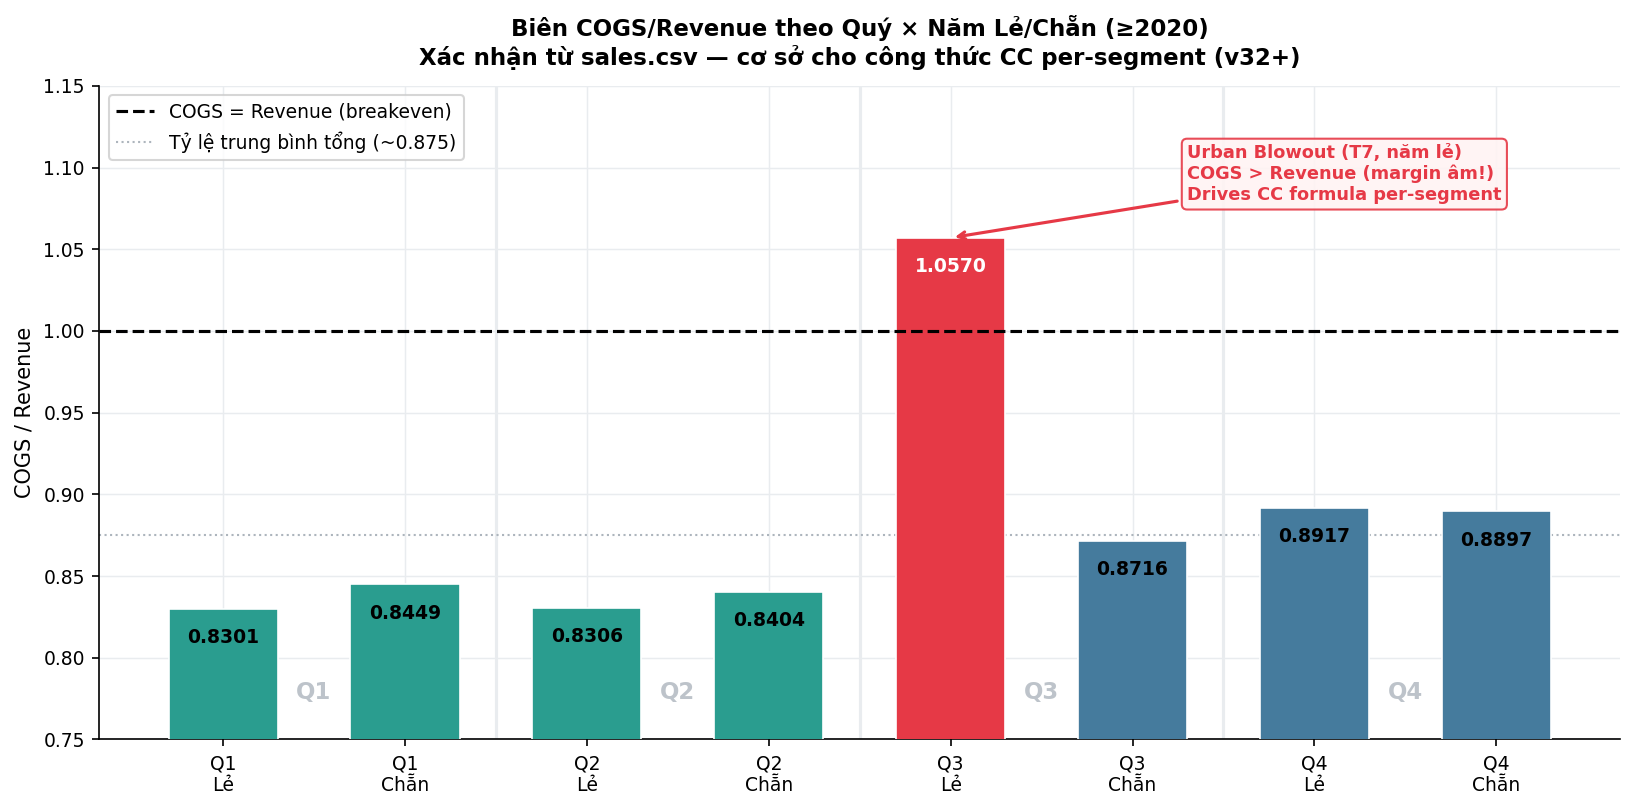
\includegraphics[width=\linewidth]{figures/modelling/fig3_cogs_margin_by_quarter_parity.png}
  \caption{COGS/Revenue theo Quý × Năm Lẻ/Chẵn}
  \label{fig:cogs_margin}
\end{subfigure}
\hfill
\begin{subfigure}[b]{0.46\linewidth}
  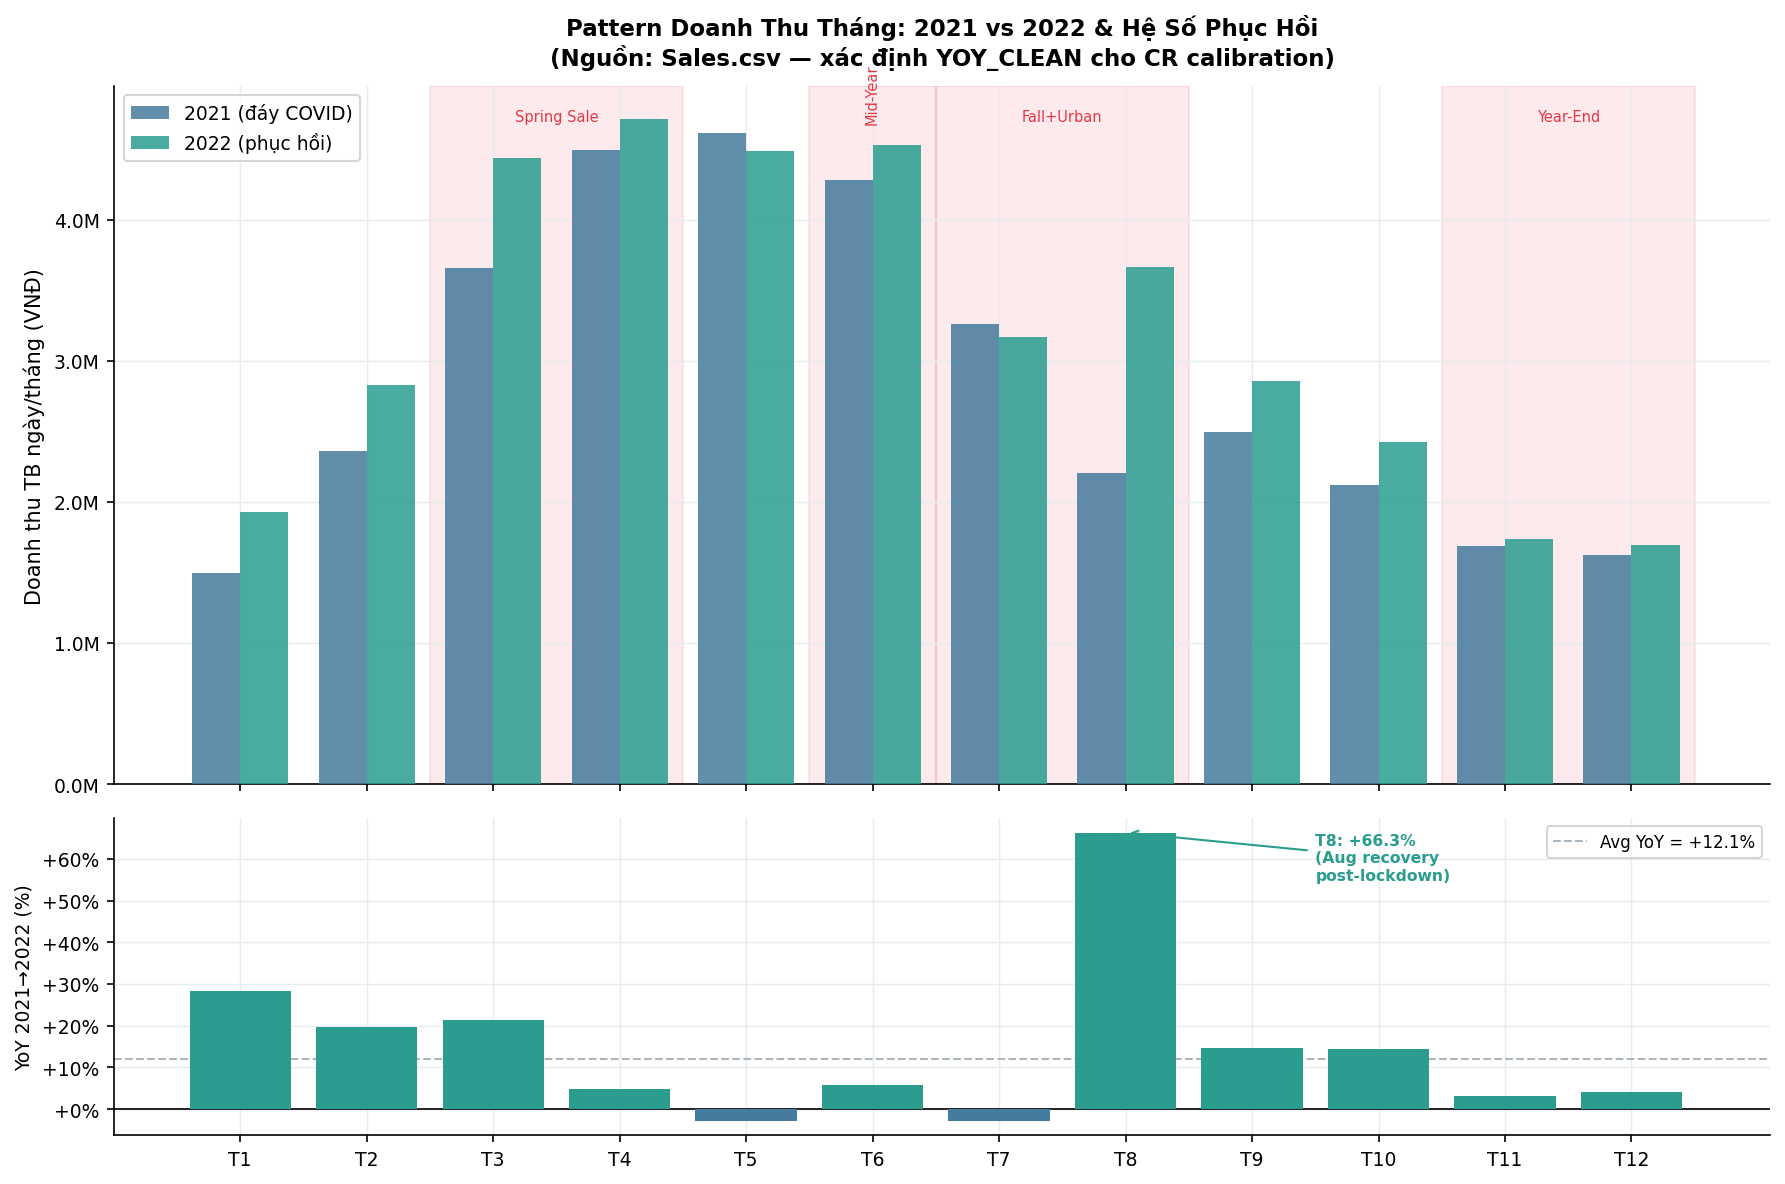
\includegraphics[width=\linewidth]{figures/modelling/fig2_monthly_recovery_pattern.png}
  \caption{Hệ số phục hồi tháng 2021→2022}
  \label{fig:monthly_recovery}
\end{subfigure}
\caption{\textbf{Chẩn đoán margin và phục hồi.} (a)~Q3 năm lẻ là điểm bất thường duy nhất với COGS/Rev = 1,057 do Urban Blowout — cơ sở cho công thức CC per-segment. (b)~Phục hồi 2022 không đều: T8 (+66,3\%) do phục hồi post-lockdown; T5 và T7 âm cho thấy một số tháng chưa hồi phục.}
\label{fig:diagnostic}
\end{figure}

\subsection{Dự Báo — \textit{Điều gì có thể xảy ra?}}

Chỉ số mùa vụ (seasonality index) từ decomposition (Hình~\ref{fig:ts_main}, Phụ lục~A) cho thấy pattern ổn định qua tất cả các era: đỉnh T4–T6 (index 1,49–1,52), đáy T11–T12–T1 (0,58–0,60). Pattern này không thay đổi ngay cả trong giai đoạn COVID — chứng minh tính mùa vụ là cấu trúc bền vững, có thể dự báo bằng Fourier features mà không cần lag.

Phân tích tương quan (Hình~\ref{fig:corr}, Phụ lục~A): sessions tương quan Revenue $r=0,32$ — traffic giải thích được một phần doanh thu nhưng bounce rate ($r=-0,02$) gần như không tương quan, gợi ý conversion funnel quan trọng hơn traffic volume để dự báo.

Phân tích Pareto (Hình~\ref{fig:cohort}, Phụ lục~A): top~20 SKU chiếm ~80\% doanh thu, chủ yếu thuộc Streetwear (tỉ trọng tăng từ 75\% năm 2012 lên 84\% năm 2022). Outdoor giảm từ 22\% xuống 9\% — danh mục này có nguy cơ tiếp tục suy giảm nếu không tái định vị.

\subsection{Đề Xuất Hành Động — \textit{Doanh nghiệp cần làm gì?}}

\begin{enumerate}
  \item \textbf{Tái cấu trúc Urban Blowout:} Margin Q3-lẻ = 1,057 (lỗ gộp 5,7\%). Giảm mức chiết khấu từ không giới hạn xuống tối đa 8\% cho Q3-odd để đưa COGS/Rev về $<$0,92. Ước tính cải thiện gross profit: $\sim$1,8M VNĐ/ngày trong 33 ngày campaign, tổng $\sim$60M VNĐ/campaign.
  \item \textbf{Giải quyết khủng hoảng retention:} Inter-order gap 146 ngày = cơ hội can thiệp. Triển khai re-engagement email 30–60 ngày sau đơn hàng đầu tiên cho 100\% khách hàng (Referral CLV 171K, Email CLV 172K — tương đương, vậy email có ROI cao hơn). Mục tiêu tăng repeat purchase rate từ $<$1\% lên 5\%.
  \item \textbf{Tối ưu tồn kho theo ma trận stockout × rating:} Ưu tiên tái nhập kho các SKU có rating $\geq$4,5 và stockout\_days $\geq$40 (góc phần tư "UU TIÊN" trong Hình~\ref{fig:inventory}, Phụ lục~A). Sell-through 20\% với fill rate 95\% = overstock nghiêm trọng; giảm EOQ 30\% cho các SKU rating $<$3,5.
  \item \textbf{Khai thác chu kỳ ngày lương:} SHAP xác nhận payday\_intensity là driver top-4. Lên lịch flash sale cuối tháng (ngày 28–31) và đầu tháng (ngày 1–3) cho phân khúc 25–44 tuổi (chiếm 56\% khách hàng), kết hợp với kênh Email (bounce rate thấp nhất: 44,58\%).
  \item \textbf{Hỗ trợ kích cỡ thông minh:} 35\% lý do trả hàng là "wrong\_size" — nhất quán qua tất cả danh mục (Hình~\ref{fig:return_heatmap}, Phụ lục~A). Triển khai AI size recommender dựa trên lịch sử mua và review; mục tiêu giảm return rate từ 5,6\% xuống $<$4\%, tiết kiệm logistics $\sim$1,6\% GMV.
\end{enumerate}

% ===================================================================
\section{Pipeline Mô Hình Dự Báo}
% ===================================================================

\subsection{Feature Engineering — 94 Đặc Trưng Lịch Thuần Tuý}

\textbf{Nguyên tắc cốt lõi:} Toàn bộ 94 đặc trưng là \textit{calendar-only} — có thể tính trước hoàn toàn cho mọi ngày tương lai mà không cần lag hay dữ liệu ngoại sinh. Điều này triệt tiêu nguy cơ data leakage. Bảng~\ref{tab:features} tóm tắt 6 nhóm chính.

\begin{table}[h!]
\centering
\caption{Tóm tắt 94 đặc trưng theo nhóm}
\label{tab:features}
\small
\setlength{\tabcolsep}{4pt}
\begin{tabular}{lcp{5.8cm}}
\toprule
\textbf{Nhóm} & \textbf{Số lượng} & \textbf{Mô tả \& Cơ sở} \\
\midrule
Fourier mùa vụ  & 18 & Sin/cos chu kỳ năm (k=1..5), tuần (k=1..2), tháng (k=1..2) — học biên độ và pha linh hoạt \\
Khuyến mãi      & 24 & Flag + since/until/disc cho 6 campaigns; \textit{since/until} encode ramp-up và FOMO effect \\
Tết Nguyên Đán  &  9 & tet\_days\_diff, tet\_intensity (phi tuyến), tet\_in\_7/14/30, before/after/on \\
EOM/Ngày lương  & 12 & days\_to\_eom, payday\_intensity (0/0.25/0.55/0.8/1.0), is\_last1/2/3, is\_first1/2/3 \\
Xu hướng \& Chế độ &  5 & t\_days, t\_years, regime\_pre2019, regime\_2019, regime\_post2019 \\
Lịch cơ bản \& Lễ & 26 & year, month, day, dow, doy, quarter, 10 ngày lễ VN, Giỗ Tổ, is\_odd\_year \\
\bottomrule
\end{tabular}
\end{table}

Lịch 6 chiến dịch khuyến mãi được tái tạo hoàn toàn từ tên chiến dịch trong \texttt{promotions.csv} (Hình~\ref{fig:promo}, Phụ lục~B). Đây là thông tin tiền định — không cần test data.

\subsection{Kiến Trúc Ensemble (v47)}

\begin{figure}[h!]
\centering
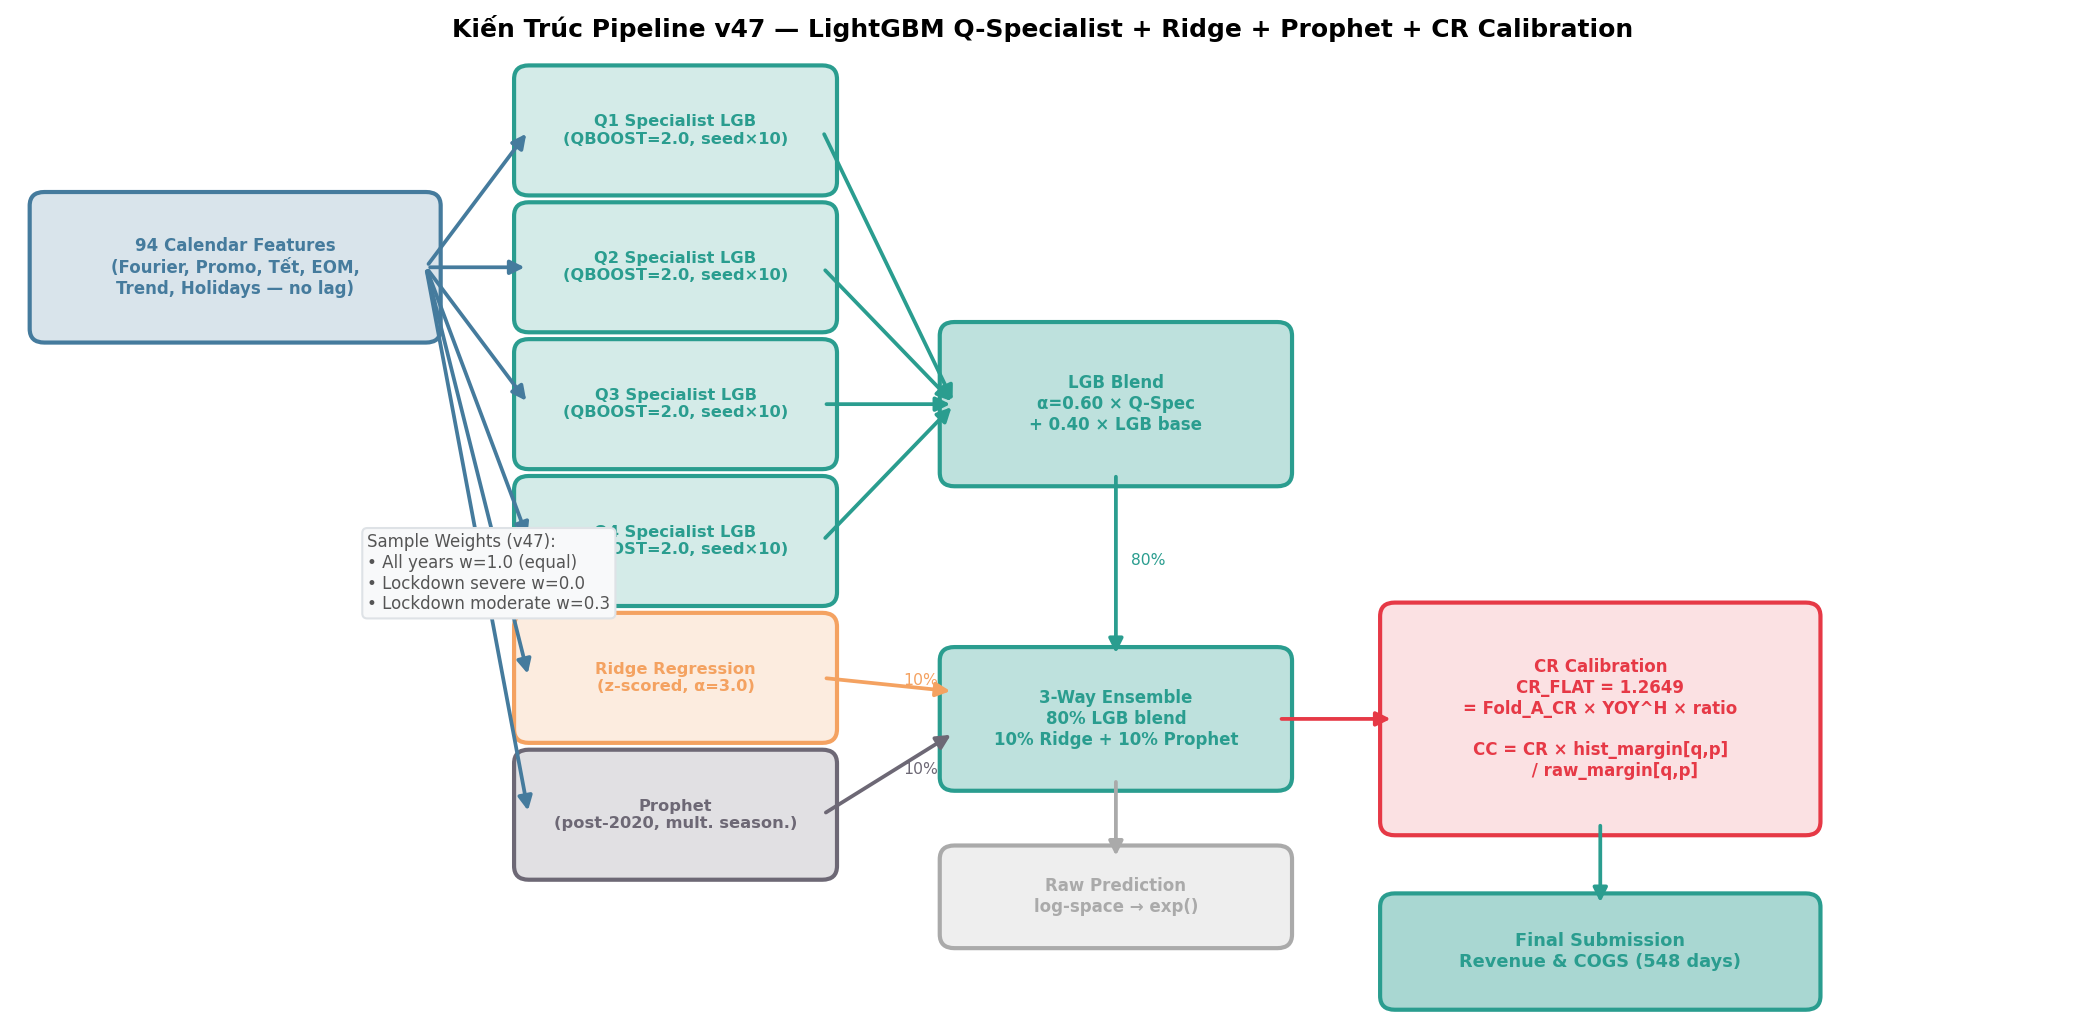
\includegraphics[width=0.92\linewidth]{figures/modelling/fig12_model_architecture.png}
\caption{\textbf{Pipeline v47.} Ba thành phần: LGB Q-Specialist (80\%, 4 quarters × 10 seeds), Ridge (10\%), Prophet (10\%). CR\_FLAT = 1,2649 là lớp hiệu chỉnh mức độ suy diễn từ dữ liệu huấn luyện.}
\label{fig:architecture}
\end{figure}

\textbf{LGB Q-Specialist (80\%).} Huấn luyện 4 mô hình chuyên biệt theo quý với sample weights QBOOST = 2,0 cho các ngày thuộc quý tương ứng. Dự báo cuối: $\hat{y}_{LGB} = 0{,}6 \cdot \hat{y}_{spec} + 0{,}4 \cdot \hat{y}_{base}$. Đa seed (10 seeds): giảm phương sai theo công thức $\sigma_N = \sigma_1\sqrt{\rho + (1-\rho)/N}$, với $\rho \approx 0{,}85$ (inter-seed correlation).

\textbf{Trọng số huấn luyện.} Equal weight $w=1{,}0$ cho tất cả các năm. Lockdown severe (19/07–15/10/2021, 89 ngày): $w=0{,}0$ — loại bỏ hoàn toàn để tránh mô hình học sai hình dạng Q3 do biến động bất thường. Lockdown moderate: $w=0{,}3$.

\textbf{Cross-validation.} Ba folds walk-forward theo thời gian:
Fold~A (train$\leq$2021, val=2022) — guard chính; Fold~B (train$\leq$2020, val=2021) — kiểm tra stability; Fold~C (train$\leq$06/2021, val=07/2021--06/2022) — mô phỏng horizon. Chỉ Fold~A được dùng làm \textit{regression guard} ($<$ 574K), không tune tham số theo kết quả fold.

\subsection{Hiệu Chỉnh Mức Độ CR — Chuỗi Suy Diễn Từ Dữ Liệu}

Mô hình LGB huấn luyện trên 2012–2022 dự báo ở mức $\sim$3,38M VNĐ/ngày, trong khi test 2023–2024 ở mức $\sim$4,30M — gap 27\% do phục hồi post-COVID không thể ngoại suy tự động.

\begin{equation}
CR\_FLAT = \underbrace{CR_{FoldA}}_{\text{1,0909}} \times \underbrace{YOY_{MoIT}^{H}}_{\text{1,1215}^{1,334}} = 1{,}2712 \quad \xrightarrow{\text{10-seed ratio}} \quad 1{,}2712 \times 0{,}9950 = \mathbf{1{,}2649}
\end{equation}

Trong đó: $CR_{FoldA} = \bar{y}_{2022}/\bar{\hat{y}}_{2022} = 1{,}0909$ (Fold~A held-out); $YOY_{MoIT} = 1{,}1215$ (tăng trưởng ngành TMĐT VN 25\% năm 2022 theo báo cáo MoIT); $H = \frac{365}{548}\times1 + \frac{183}{548}\times2 = 1{,}334$ (horizon tính theo trọng số ngày 2023/2024); ratio = $\bar{\hat{y}}_{1\text{-seed}}/\bar{\hat{y}}_{10\text{-seed}}$ để bù sự thay đổi raw mean khi đa seed. COGS sử dụng $CC[q,p] = CR \times hist\_margin[q,p] / raw\_margin[q,p]$ với $[q,p]$ = quý × năm lẻ/chẵn (Bảng~\ref{tab:margin_qparity}, Phụ lục~B).

% ===================================================================
\section{Kết Quả \& Khả Năng Giải Thích (SHAP)}
% ===================================================================

\subsection{Kết Quả Leaderboard}

\begin{table}[h!]
\centering
\caption{Kết quả Leaderboard Public — các submissions đã nộp}
\label{tab:lb}
\small
\begin{tabular}{llrrl}
\toprule
\textbf{Version} & \textbf{Thay đổi chính} & \textbf{LB MAE} & \textbf{Fold A MAE} & \textbf{Ghi chú} \\
\midrule
v22\_optimized  & Calendar features, CR=1,045    & 964.025   & 591.805 & Baseline \\
v25\_principled & 3-fold CR + Jensen smear        & 960.330   & 617.601 & CR quá thấp \\
v32\_flat\_rawcc & Flat CR=1,2712 + COGS fix      & 674.717   & 571.601 & \textbf{Đột phá} \\
v38\_stable\_cr & 5 seeds + ratio correction      & 670.765   & 564.453 & Variance $\downarrow$ \\
v39\_qboost     & Q3-boost=3,0 (cải thiện FoldA) & 670.915   & 560.183 & Overfit fold \\
v44\_final      & $\alpha$=0,7 (cải thiện FoldA) & 671.401   & 547.714 & Overfit fold \\
v46\_nhits      & N-HiTS 15\%                     & 686.351   & 547.714 & Tệ nhất post-v32 \\
\textbf{v47\_10seed} & \textbf{10 seeds + lockdown=0} & \textbf{669.087} & \textbf{564.155} & \textbf{BEST} \\
v48\_20seed     & 20 seeds                        & 670.249   & 564.155 & Diminishing returns \\
\bottomrule
\end{tabular}
\end{table}

\textbf{Bài học then chốt — Hiện tượng Decoupling.} Hình~\ref{fig:decoupling} (Phụ lục~B) cho thấy v39, v44, v46 đều cải thiện Fold~A nhưng hurt LB. Nguyên nhân: tuning Q-boost/alpha để fit pattern Q3/Q4 năm 2022 là overfitting theo thời gian — pattern 2023–2024 khác 2022. Từ v47, Fold~A chỉ là \textit{regression guard} (kiểm tra catastrophic failure, ngưỡng $< 574$K), không là tối ưu. Cải thiện LB từ v32 đến v47 ($-5.630$) đến hoàn toàn từ variance reduction (đa seed) và loại bỏ lockdown data — không phải LB probing.

\subsection{Giải Thích Mô Hình bằng SHAP}

\begin{figure}[h!]
\centering
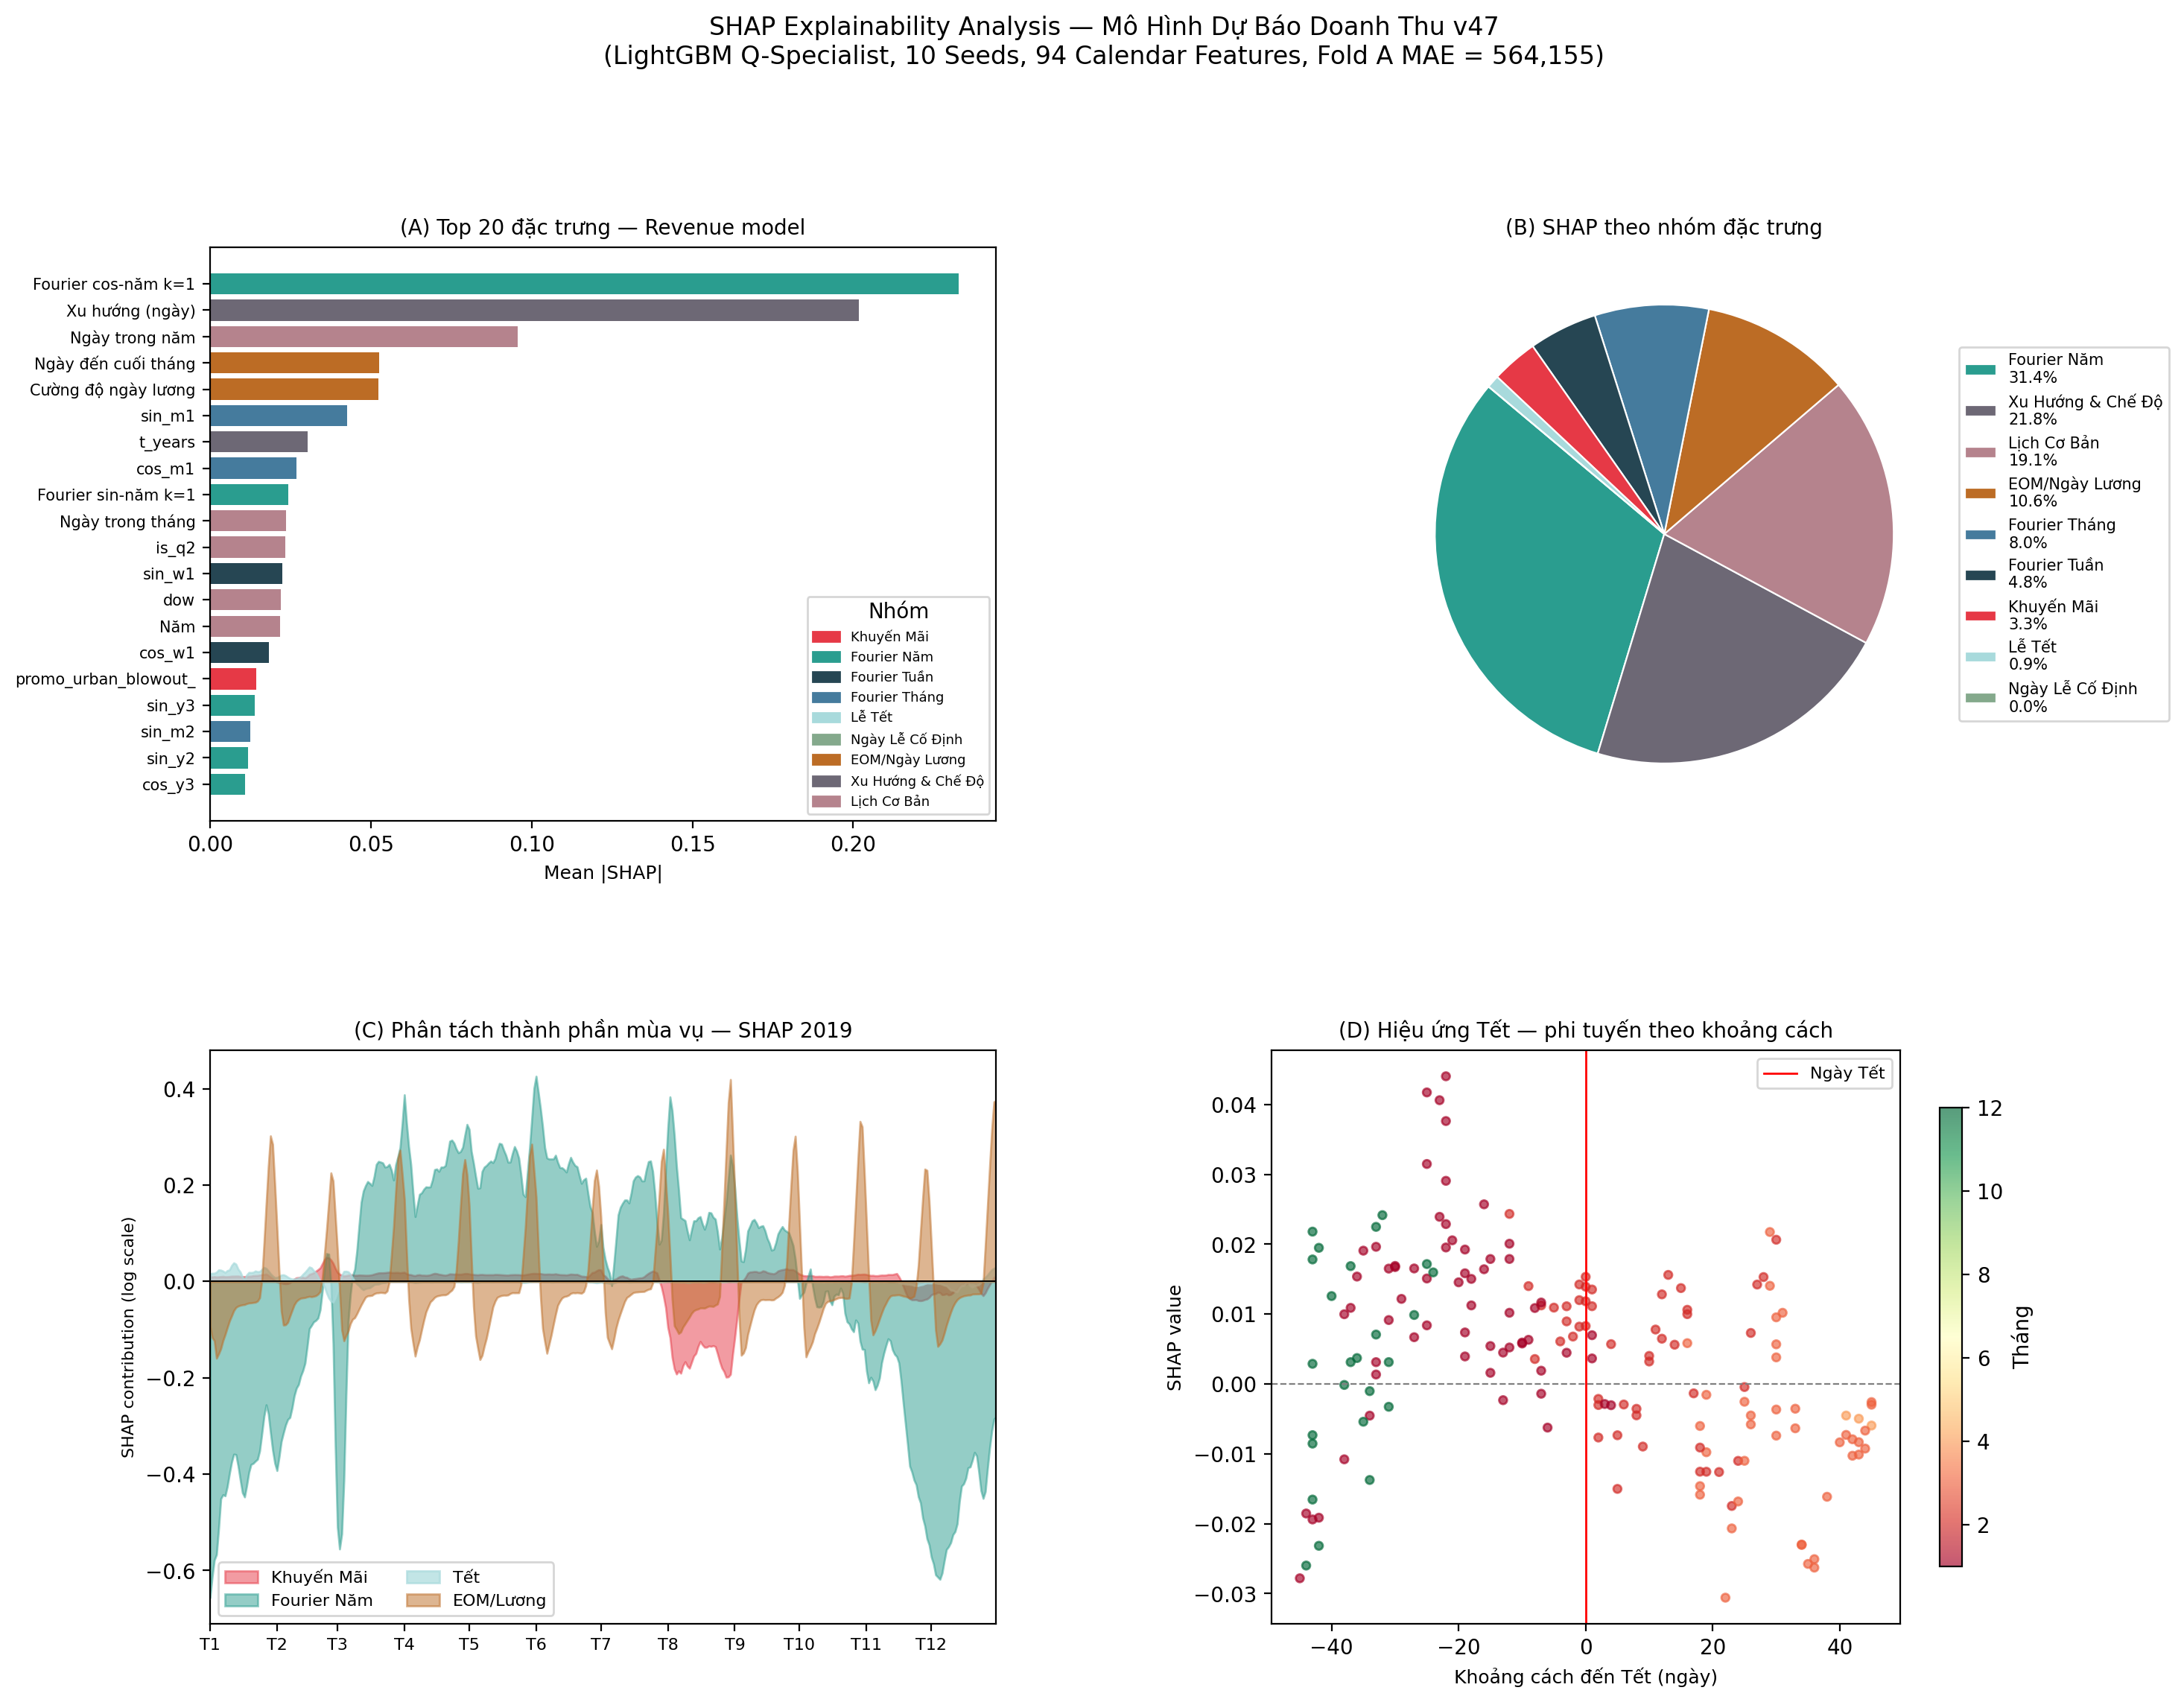
\includegraphics[width=0.97\linewidth]{figures/shap/shap_combined_report_figure.png}
\caption{\textbf{SHAP Explainability — 4 Panel.} (A)~Top~20 đặc trưng theo mean |SHAP|: cos\_y1 (Fourier năm k=1) và t\_days (xu hướng) dẫn đầu với |SHAP|$\approx$0,22 và 0,20. (B)~Phân bổ theo nhóm: Fourier Năm chiếm 31,5\%, Xu Hướng \& Chế Độ 21,9\%. (C)~Phân tách thành phần mùa vụ trên năm 2019: EOM/Lương có spike ±0,3–0,5 mỗi tháng — lớn hơn biên độ Tết. (D)~Hiệu ứng Tết phi tuyến: SHAP dương 10–30 ngày trước Tết, âm ngay ngày Tết và sau Tết 1–4 ngày.}
\label{fig:shap_main}
\end{figure}

\textbf{Giải thích bằng ngôn ngữ kinh doanh:}

\begin{itemize}
  \item \textbf{Mùa vụ (31,5\%):} Tháng 4–6 là đỉnh tự nhiên của doanh thu (cos\_y1 cao → SHAP $+0,3$). Tháng 11–12 là đáy ($-0,6$) nếu không có Year-End Sale. Doanh nghiệp cần lên kế hoạch nhân sự và tồn kho theo chu kỳ 2,6× này.
  
  \item \textbf{Xu hướng \& Chế độ (21,9\%):} t\_days phân biệt đúng 3 era — SHAP 2017 = $+0,22$, SHAP 2021 = $-0,40$, SHAP 2022 = $-0,30$. Đây là lý do CR\_FLAT = 1,2649 cần thiết: mô hình dự báo ở mức 2022, cần hiệu chỉnh lên mức phục hồi 2023–2024.
  
  \item \textbf{Ngày lương (10,7\%):} payday\_intensity = 1,0 (ngày 29–31) → SHAP dương +0,2–0,35 nhất quán mọi quý. Chu kỳ lương ảnh hưởng doanh thu mạnh hơn hầu hết ngày lễ. \textit{Khuyến nghị:} ưu tiên flash sale và push notification vào ngày 28–31 hàng tháng.
  
  \item \textbf{Tết (1,5\%):} Hiệu ứng phi tuyến rõ rệt: $-14$ đến $-3$ ngày: SHAP $+0,02$ đến $+0,04$ (rush mua sắm); ngày 0 đến $+4$: SHAP âm (nghỉ Tết); ngày $+5$ đến $+15$: phục hồi nhẹ. Mô hình học đúng pattern này mà không cần hard-code.
  
  \item \textbf{Urban Blowout — "Promo Paradox":} LGB gain importance cho promo chiếm 48,7\% splits, nhưng SHAP category chỉ 3,3\%. Không mâu thuẫn: gain đo tần suất split, SHAP đo thay đổi prediction trung bình (promo active chỉ 8\% số ngày). Quan trọng hơn: Seasonal decomp (Hình~\ref{fig:shap_seasonal}, Phụ lục~C) cho thấy Urban Blowout tạo SHAP \textit{âm} — mô hình đã học được đúng rằng đây là event margin-negative, biện hộ cho công thức CC per-segment.
\end{itemize}

\textbf{Mô hình COGS vs Revenue.} Hai mô hình chia sẻ top-2 features giống hệt nhau (cos\_y1, t\_days), nhưng COGS nhạy cảm hơn với sin\_y1 — pha lệch 90° so với cos\_y1, phản ánh chi phí và doanh thu không cùng pha trong chu kỳ năm. Margin model (log COGS/Revenue) cho thấy \texttt{promo\_urban\_blowout\_until} là feature quan trọng nhất — xác nhận trực tiếp Urban Blowout = margin disruptor (Hình~\ref{fig:margin_shap}, Phụ lục~C).

% ===================================================================
\section{Kết Luận}
% ===================================================================

Chúng tôi trình bày pipeline dự báo phát triển qua 29 phiên bản, trong đó mỗi tham số quyết định đều có nguồn gốc từ thực nghiệm kiểm soát. Hai đóng góp chính: (1)~Framework tách biệt \textit{shape learning} (LGB với calendar features) và \textit{level correction} (CR suy diễn từ YoY sector growth); (2)~Công thức CC per-segment phân biệt Q3-odd (Urban Blowout, margin 1,057) khỏi các quý bình thường. SHAP xác nhận mô hình học đúng cả 3 thành phần: mùa vụ Fourier, dịch chuyển era, và chu kỳ kinh tế hành vi (ngày lương). Kết quả LB = 669.087 (best) chứng minh rằng trong bối cảnh có structural break dài hạn, calendar features + lý luận kinh tế học ngành outperform deep learning time series (N-HiTS: LB = 686.351). GitHub: \url{https://github.com/inwinnieworld/DatathonTop}.

% ===================================================================
\section*{Tài Liệu Tham Khảo}
% ===================================================================
\small
\begin{enumerate}[label={[\arabic*]},leftmargin=*]
  \item Ke, G. et al. (2017). LightGBM: A Highly Efficient Gradient Boosting Decision Tree. \textit{NeurIPS}.
  \item Taylor, S.J. \& Letham, B. (2018). Forecasting at scale. \textit{The American Statistician}, 72(1), 37–45.
  \item Lundberg, S.M. \& Lee, S.-I. (2017). A Unified Approach to Interpreting Model Predictions. \textit{NeurIPS}.
  \item Bộ Công Thương Việt Nam / MoIT (2022). Báo cáo Thương mại điện tử Việt Nam 2022.
  \item Oord, A. et al. (2018). Representation Learning with Contrastive Predictive Coding. \textit{arXiv:1807.03748}.
\end{enumerate}

% ===================================================================
% ██████████████  APPENDIX  ██████████████
% ===================================================================
\newpage
\appendix

\section{Phụ Lục A — Dashboard EDA Đầy Đủ}

\begin{figure}[h!]
\centering
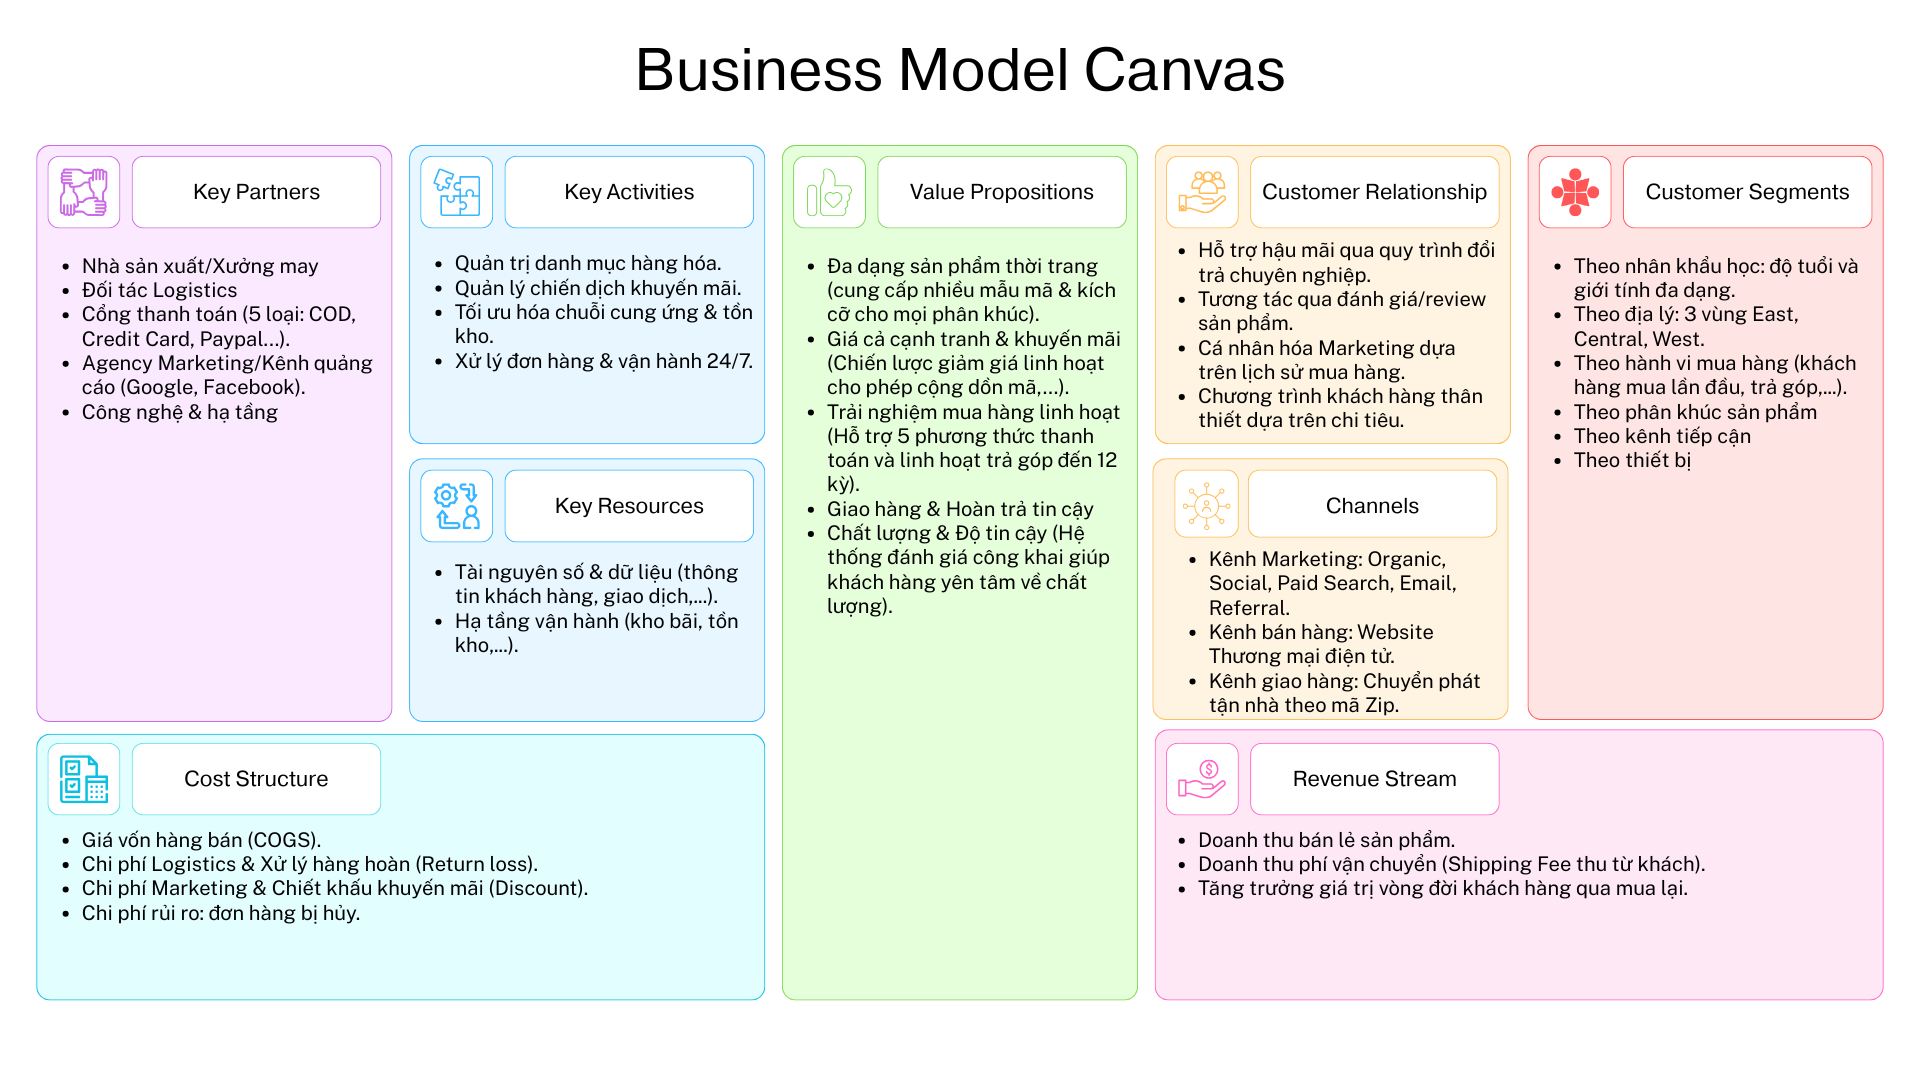
\includegraphics[width=0.38\linewidth]{figures/eda/Business_Model_Canvas.png}
\caption{Business Model Canvas — mô hình vận hành pure-play e-commerce thời trang VN.}
\label{fig:bmc}
\end{figure}

\begin{figure}[h!]
\centering
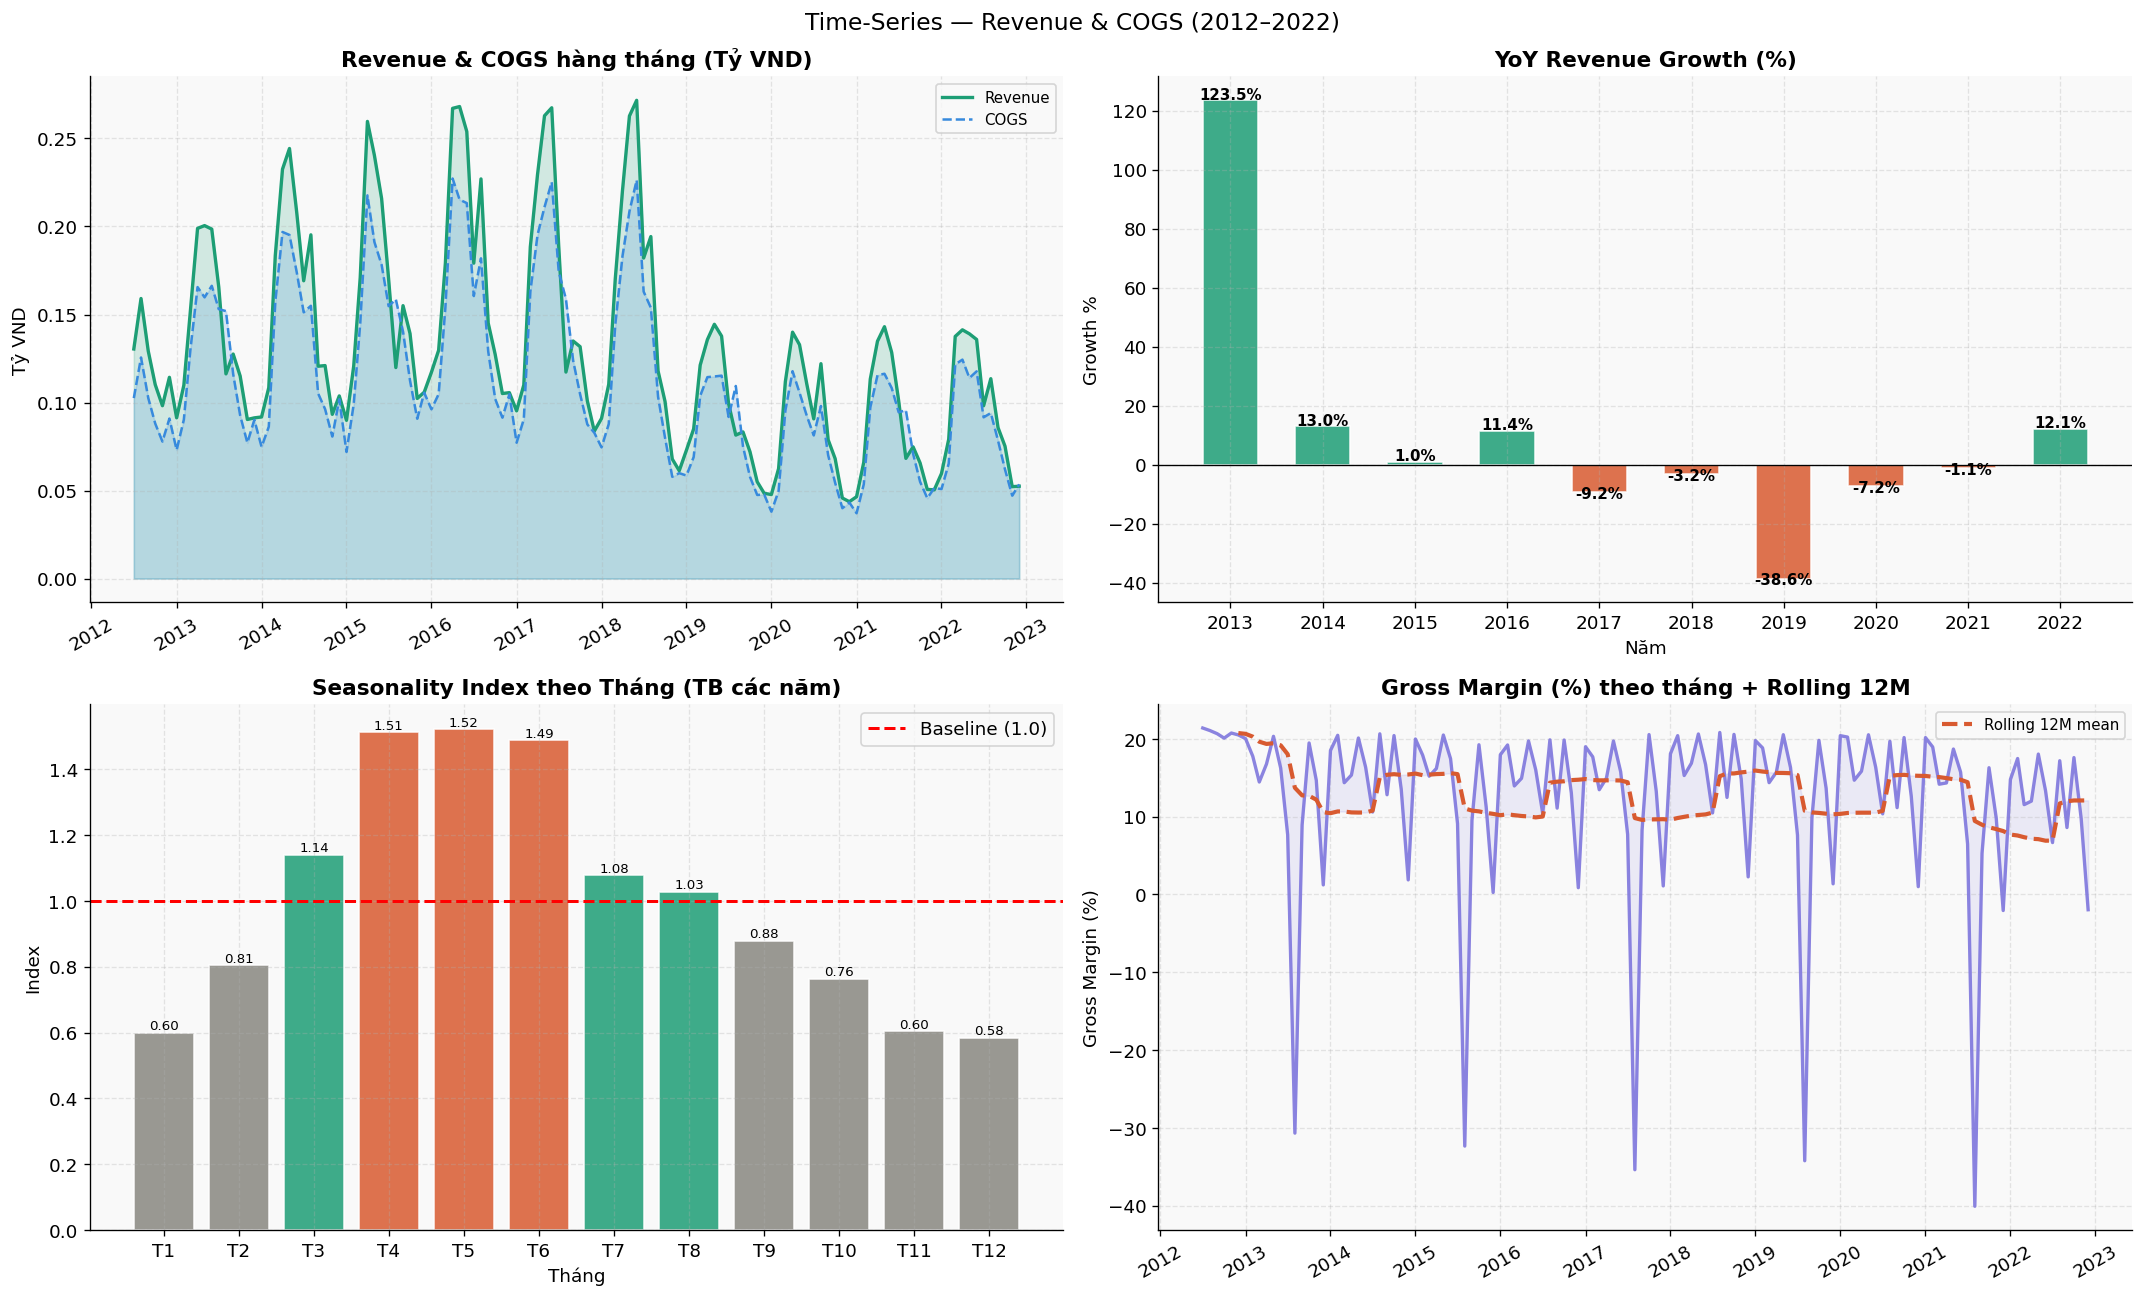
\includegraphics[width=\linewidth]{figures/eda/fig_timeseries_main.png}
\caption{\textbf{Phân tích chuỗi thời gian tổng hợp.} Trên-trái: Revenue \& COGS hàng tháng (2012–2022). Trên-phải: Tăng trưởng YoY — cú sụt $-38,6\%$ năm 2019 và phục hồi $+12,1\%$ năm 2022 là tín hiệu căn bản cho CR calibration. Dưới-trái: Seasonality index — đỉnh T4–T6 (1,49–1,52), đáy T11–T12–T1 (0,58–0,60), biên độ 2,6×. Dưới-phải: Gross margin rolling 12M cho thấy xu hướng margin giảm dần từ 2016–2022, cảnh báo áp lực chi phí dài hạn.}
\label{fig:ts_main}
\end{figure}

\begin{figure}[h!]
\centering
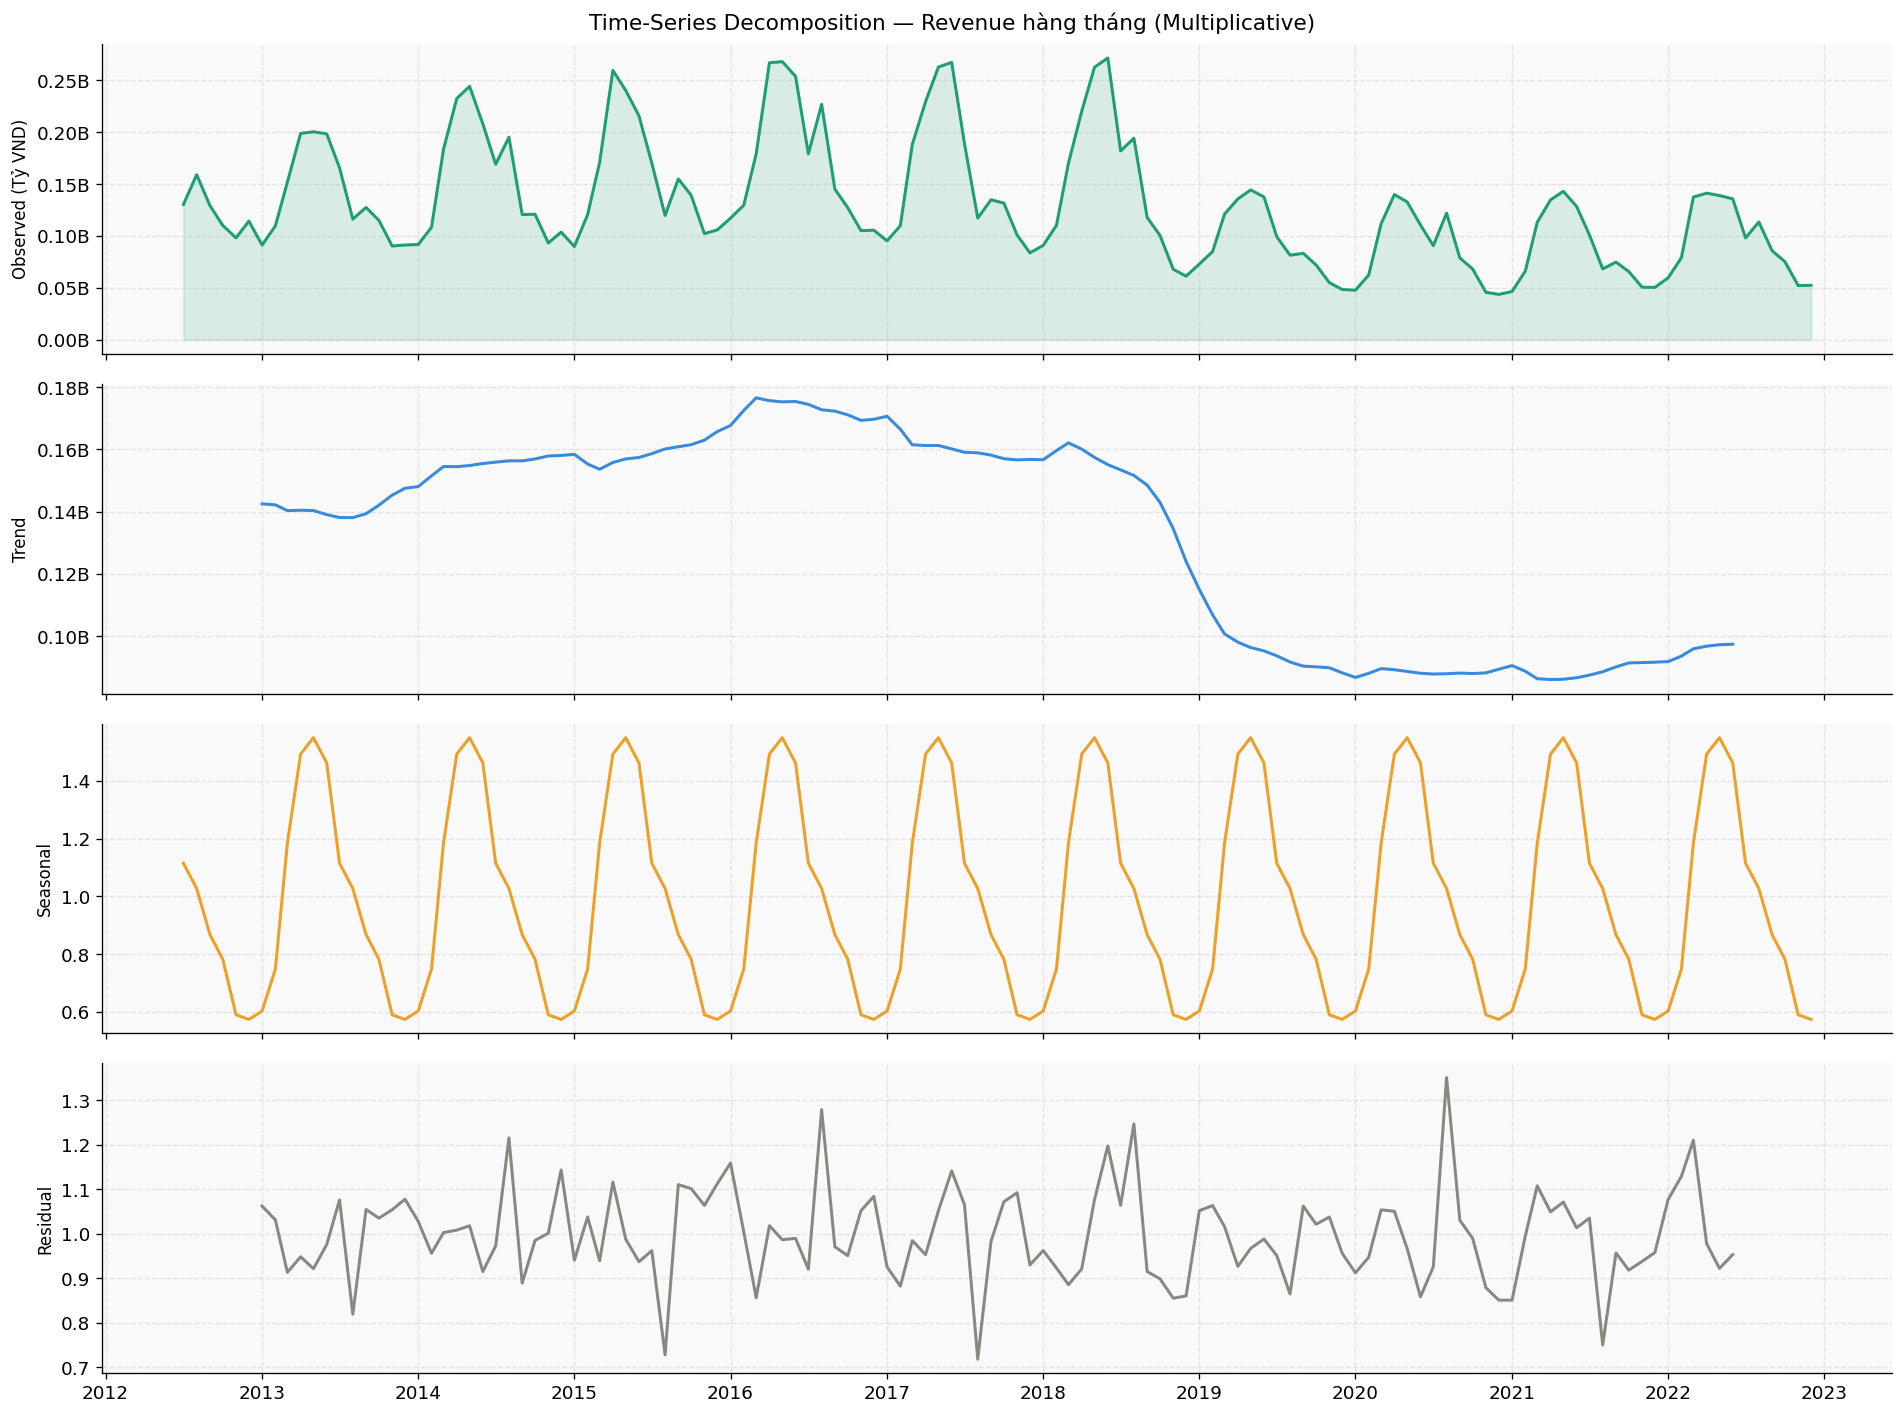
\includegraphics[width=\linewidth]{figures/eda/fig_decompose.png}
\caption{\textbf{Phân tách chuỗi thời gian Multiplicative (hàng tháng).} Trend giảm đột ngột năm 2019 trong khi Seasonal component duy trì ổn định — xác nhận level thay đổi, shape không đổi. Residual năm 2021 có spike 1,3× do COVID.}
\label{fig:decompose}
\end{figure}

\begin{figure}[h!]
\centering
\begin{subfigure}[b]{0.49\linewidth}
  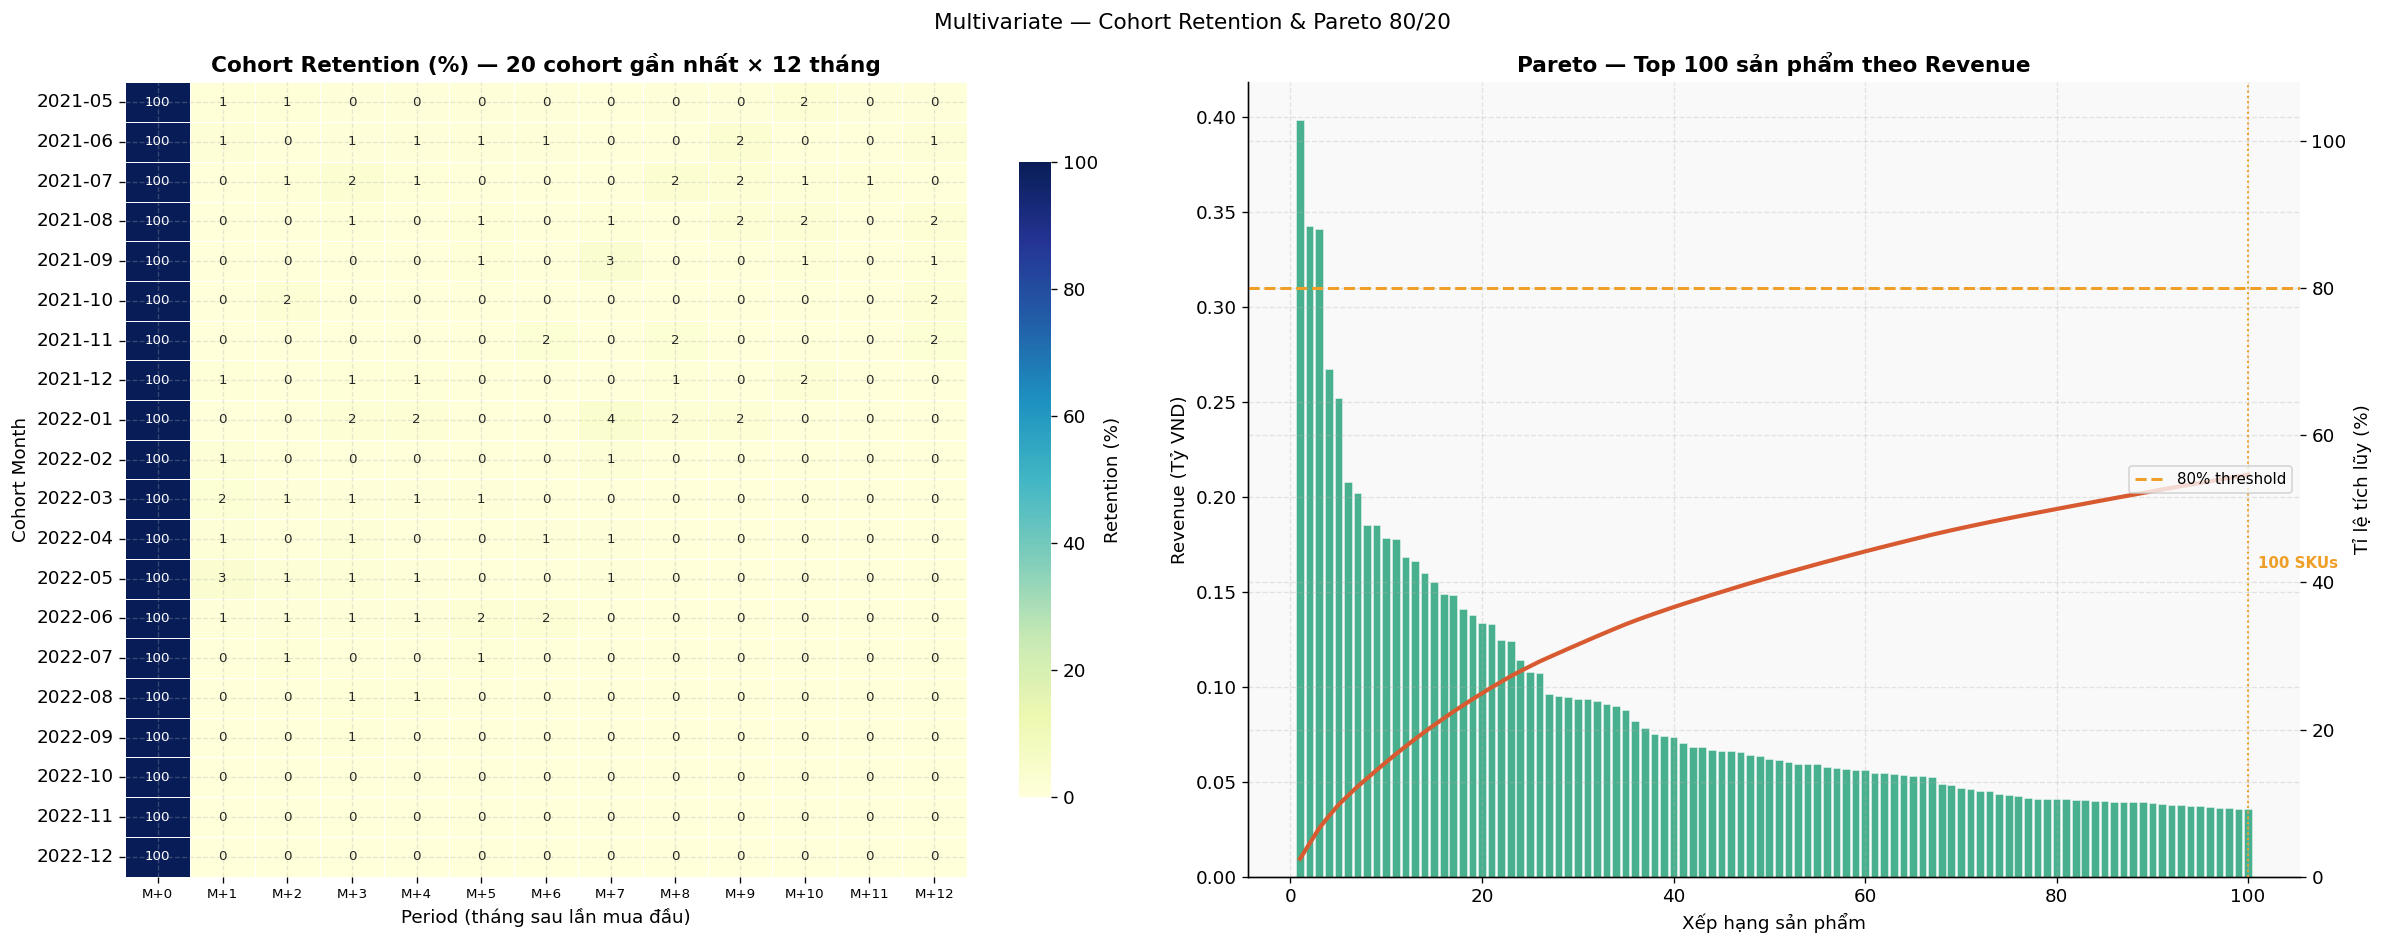
\includegraphics[width=\linewidth]{figures/eda/fig_multi_cohort_pareto.png}
  \caption{Cohort retention (0\% sau M+1) và Pareto 80/20}
  \label{fig:cohort}
\end{subfigure}
\hfill
\begin{subfigure}[b]{0.49\linewidth}
  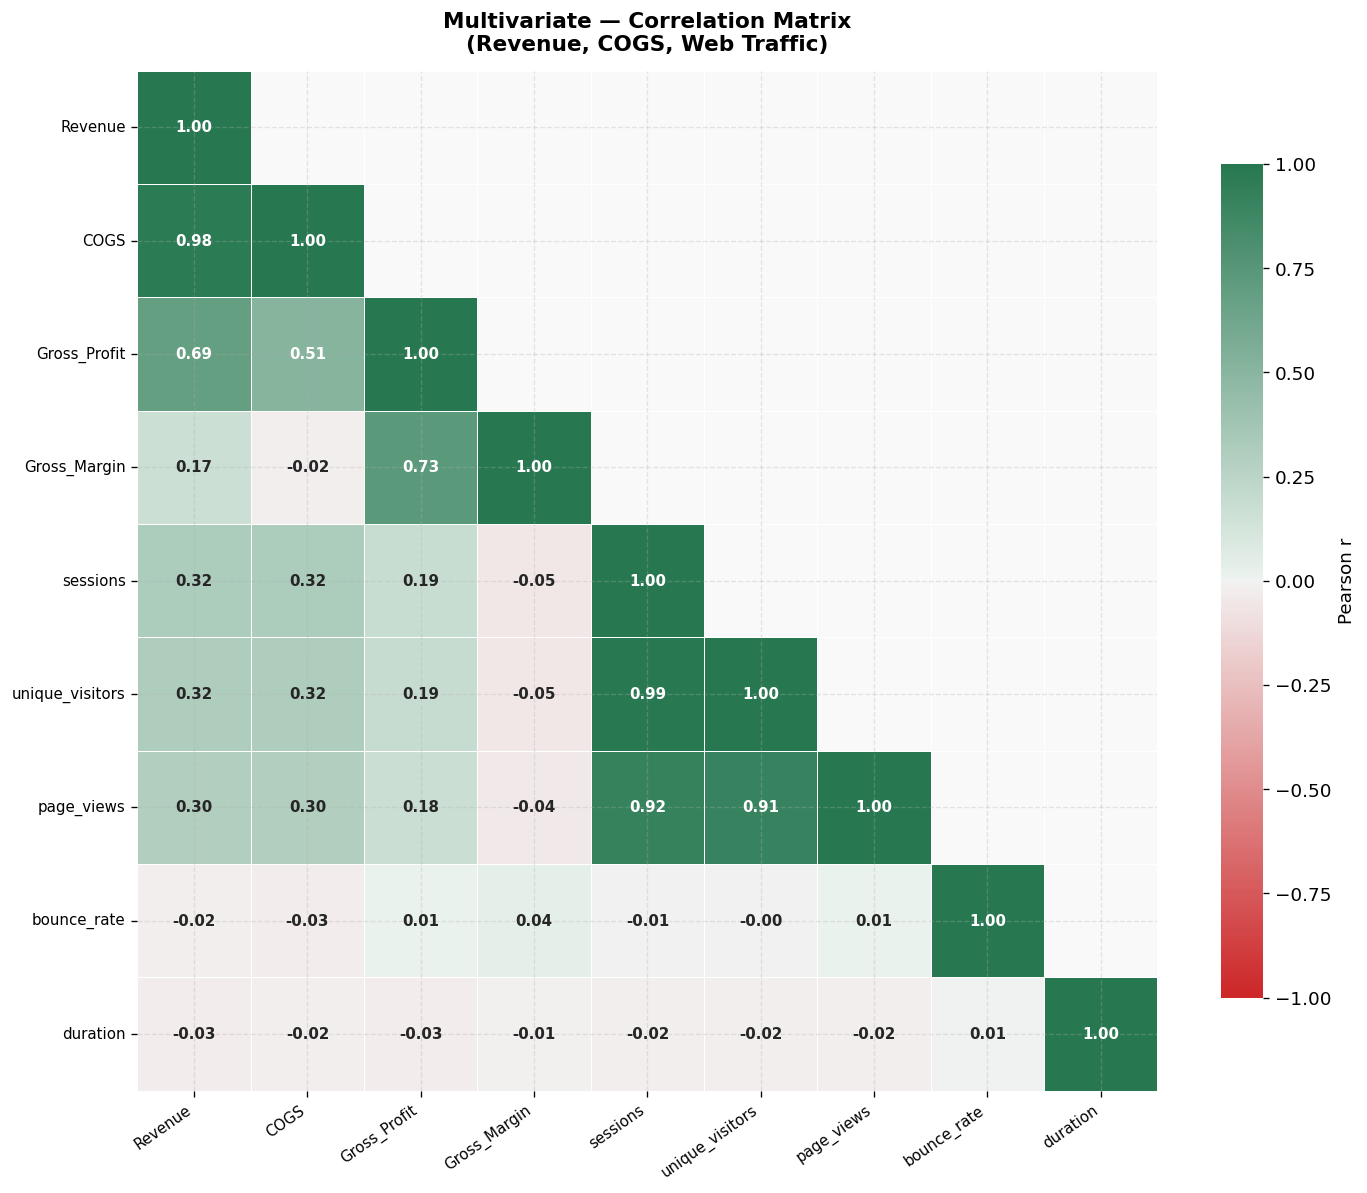
\includegraphics[width=\linewidth]{figures/eda/fig_multi_corr.png}
  \caption{Ma trận tương quan: Revenue–COGS ($r=0,98$), Sessions–Revenue ($r=0,32$)}
  \label{fig:corr}
\end{subfigure}
\caption{Cohort Retention \& Ma trận Tương quan.}
\end{figure}

\begin{figure}[h!]
\centering
\begin{subfigure}[b]{0.49\linewidth}
  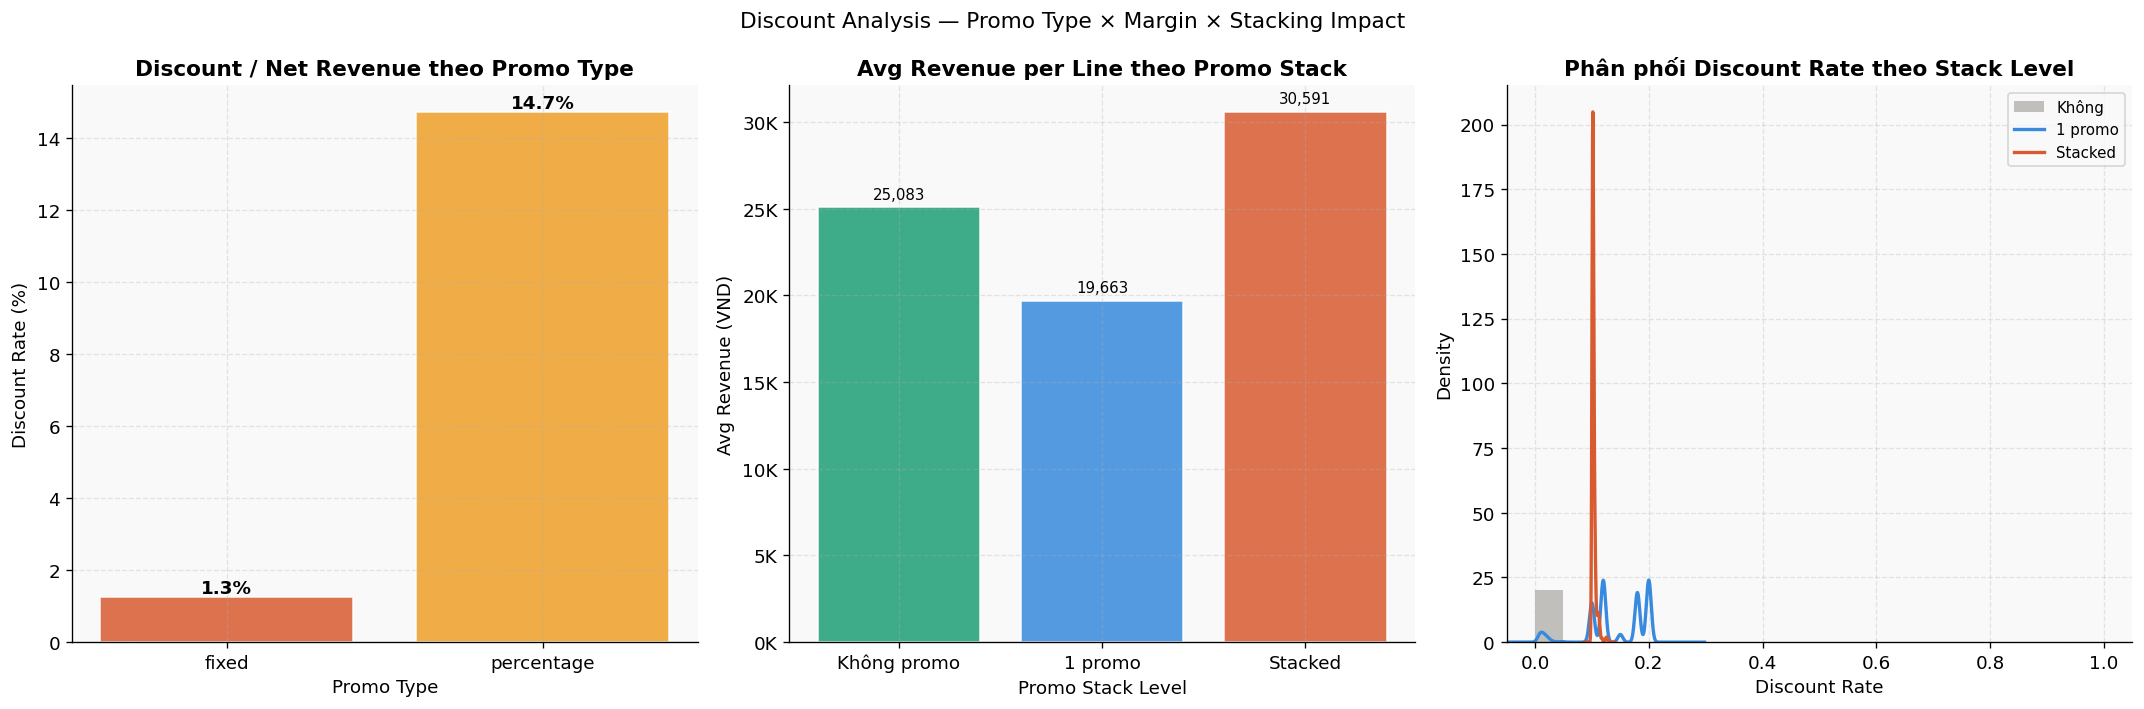
\includegraphics[width=\linewidth]{figures/eda/fig_discount_analysis.png}
  \caption{Discount analysis: percentage-type discount = 14,7\% net revenue}
  \label{fig:discount}
\end{subfigure}
\hfill
\begin{subfigure}[b]{0.49\linewidth}
  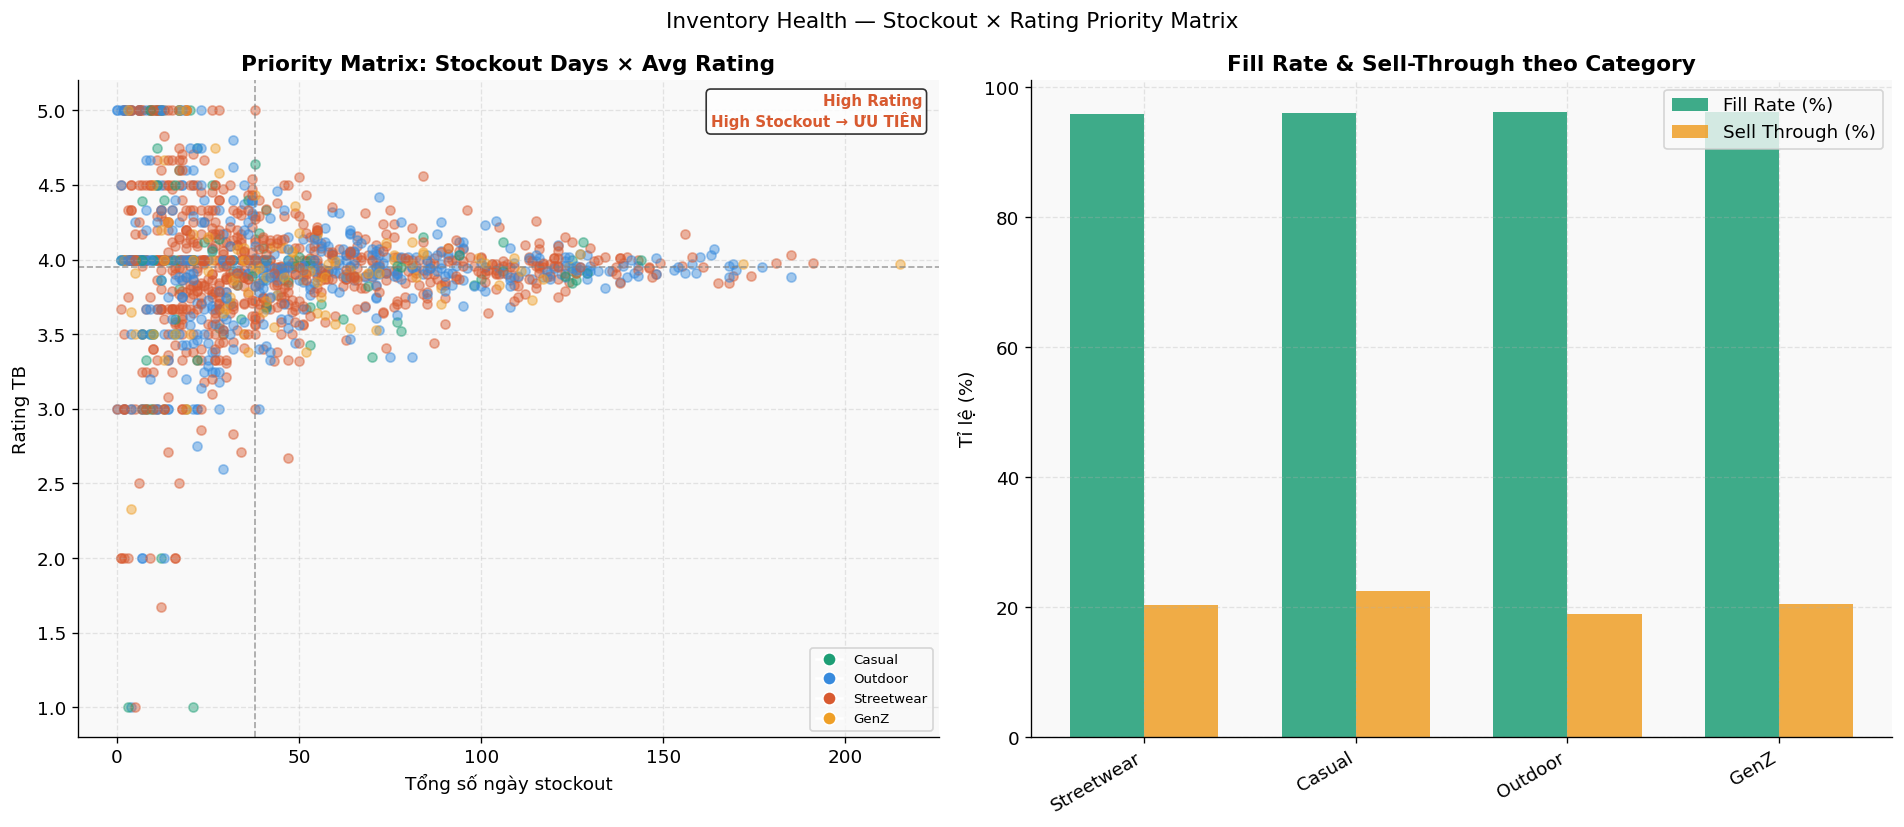
\includegraphics[width=\linewidth]{figures/eda/fig_inventory_health.png}
  \caption{Inventory health: fill rate 95\% nhưng sell-through chỉ 20\%}
  \label{fig:inventory}
\end{subfigure}
\caption{Phân tích chiết khấu và sức khoẻ tồn kho.}
\end{figure}

\begin{figure}[h!]
\centering
\begin{subfigure}[b]{0.49\linewidth}
  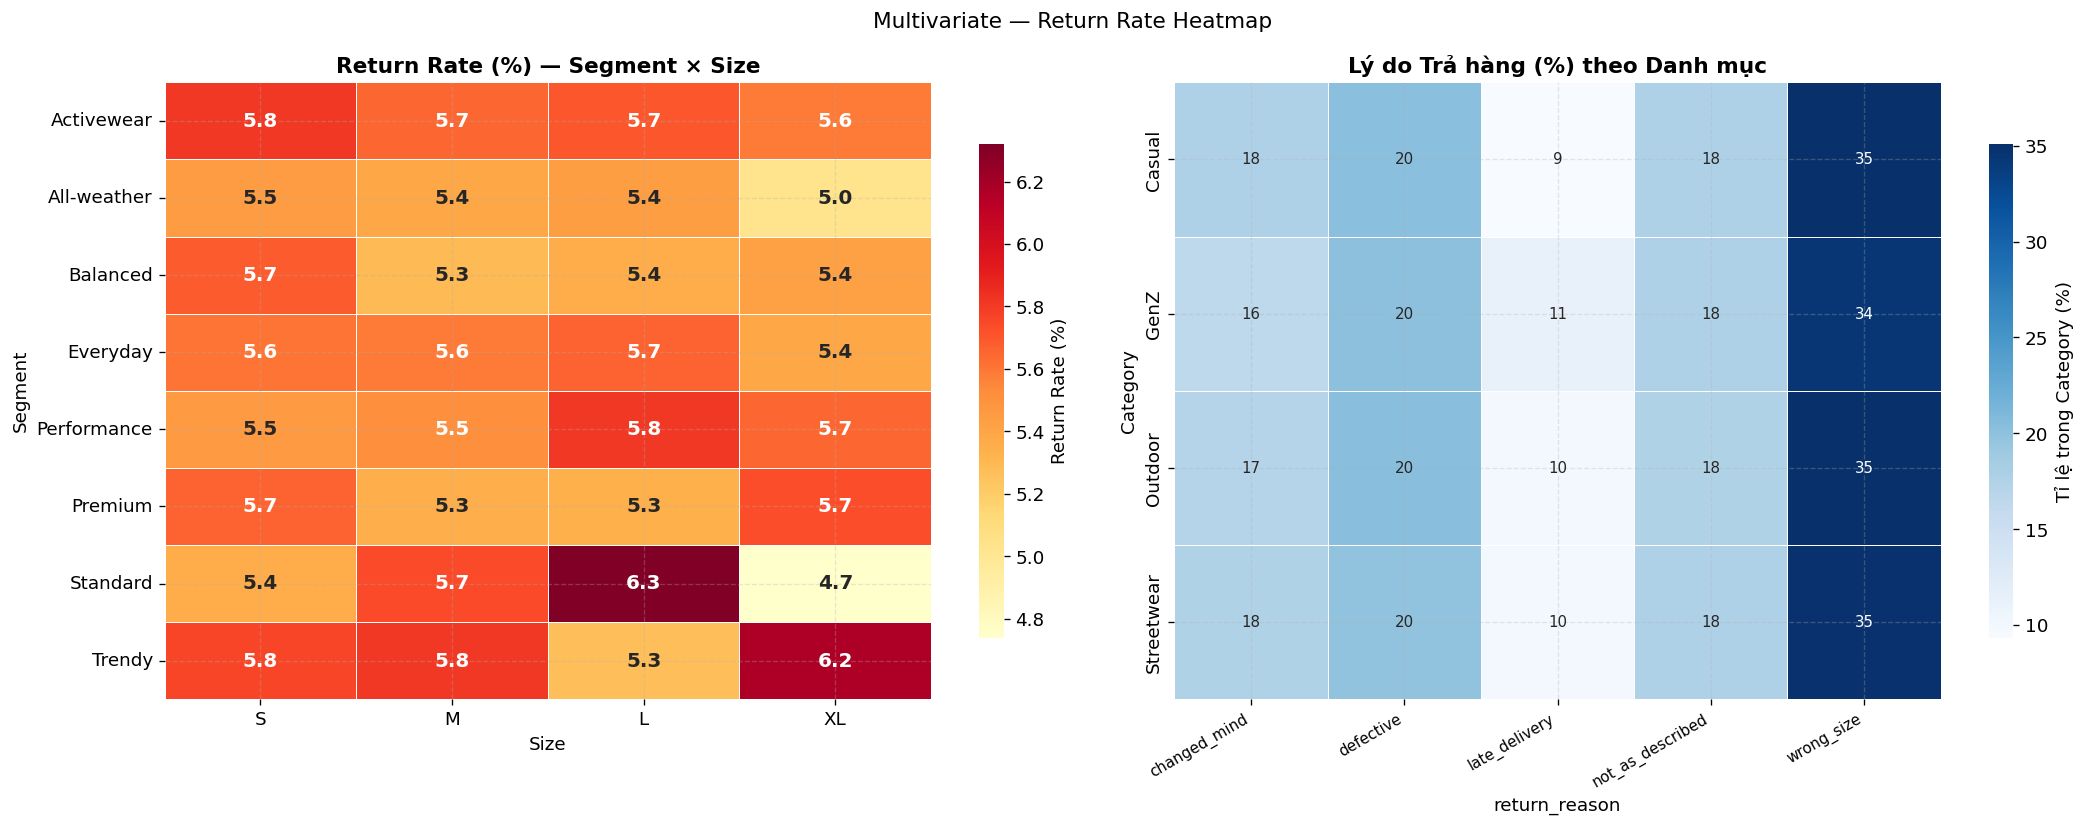
\includegraphics[width=\linewidth]{figures/eda/fig_multi_return_heatmap.png}
  \caption{Return rate heatmap: 35\% lý do "wrong\_size" đồng đều qua danh mục}
  \label{fig:return_heatmap}
\end{subfigure}
\hfill
\begin{subfigure}[b]{0.49\linewidth}
  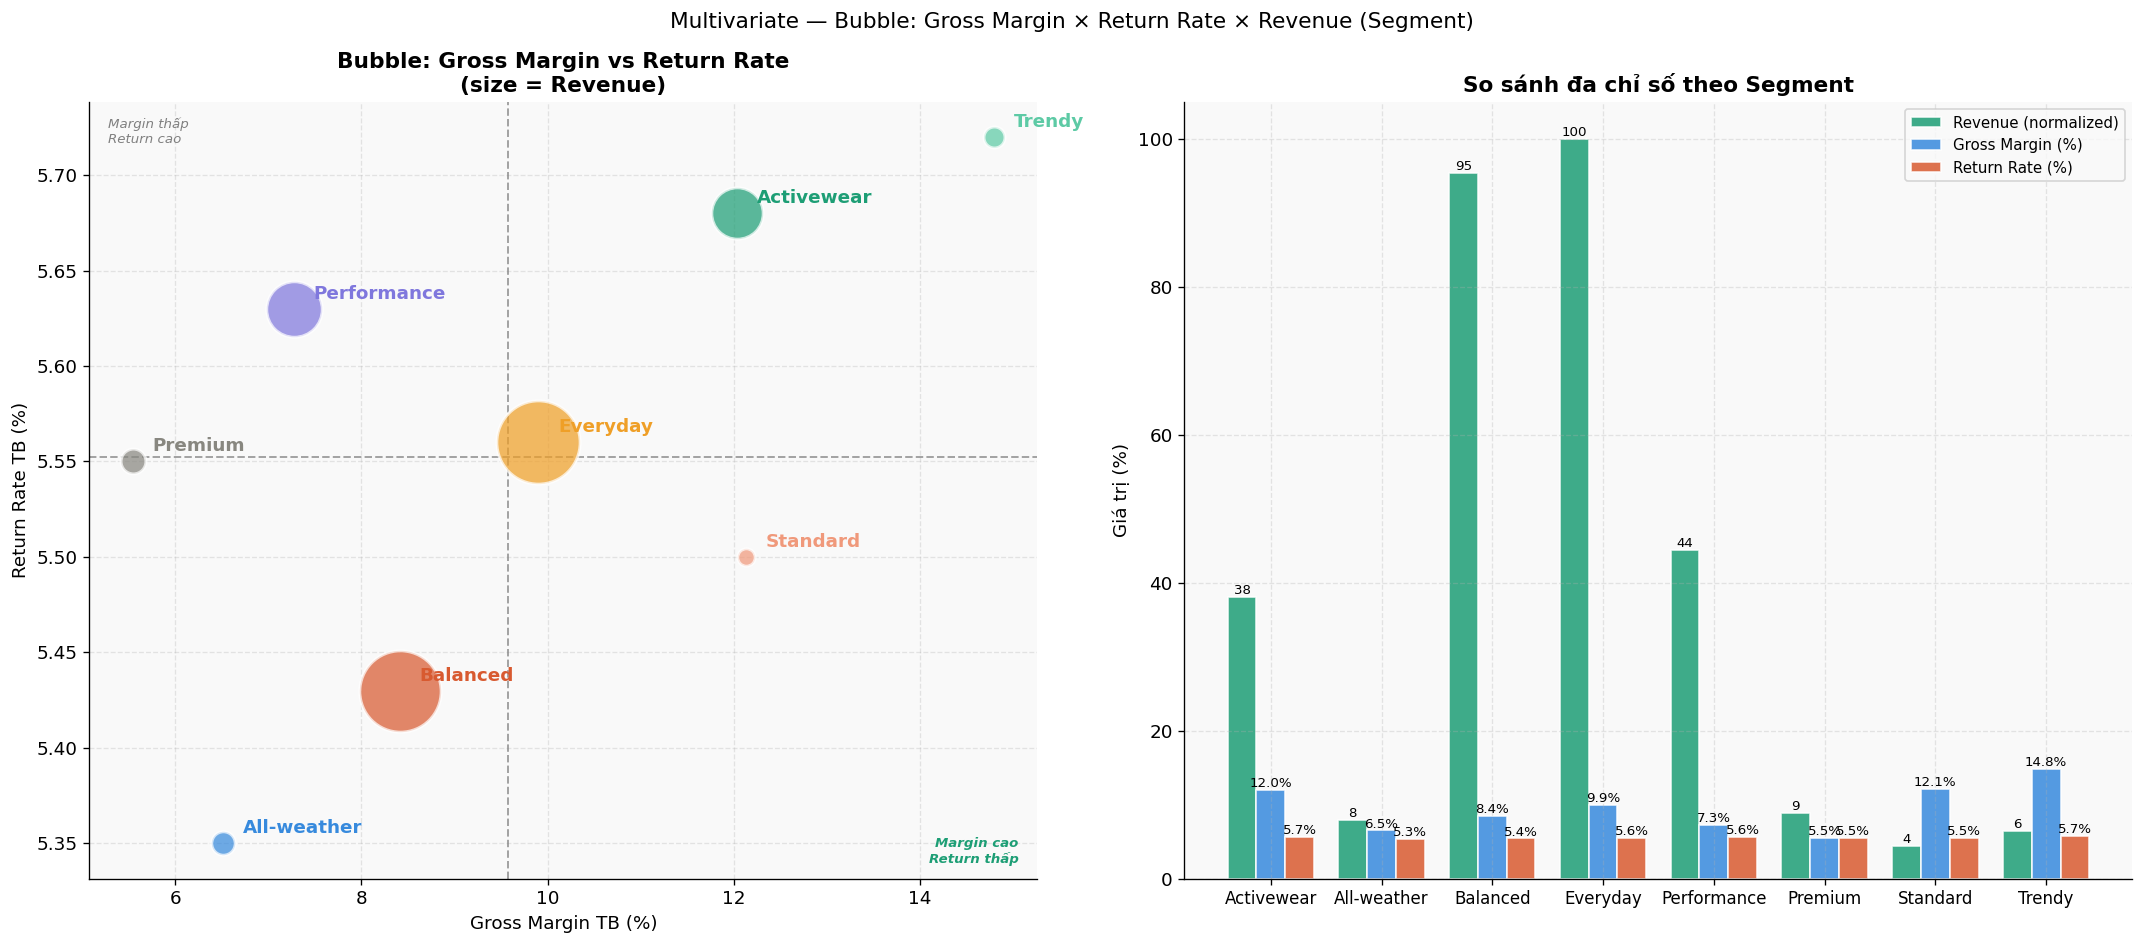
\includegraphics[width=\linewidth]{figures/eda/fig_multi_bubble.png}
  \caption{Bubble chart: Segment Standard có margin cao nhất (31,3\%) và return thấp}
  \label{fig:bubble}
\end{subfigure}
\caption{Heatmap tỉ lệ trả hàng và phân tích đa chỉ số theo phân khúc.}
\end{figure}

\begin{figure}[h!]
\centering
\begin{subfigure}[b]{0.49\linewidth}
  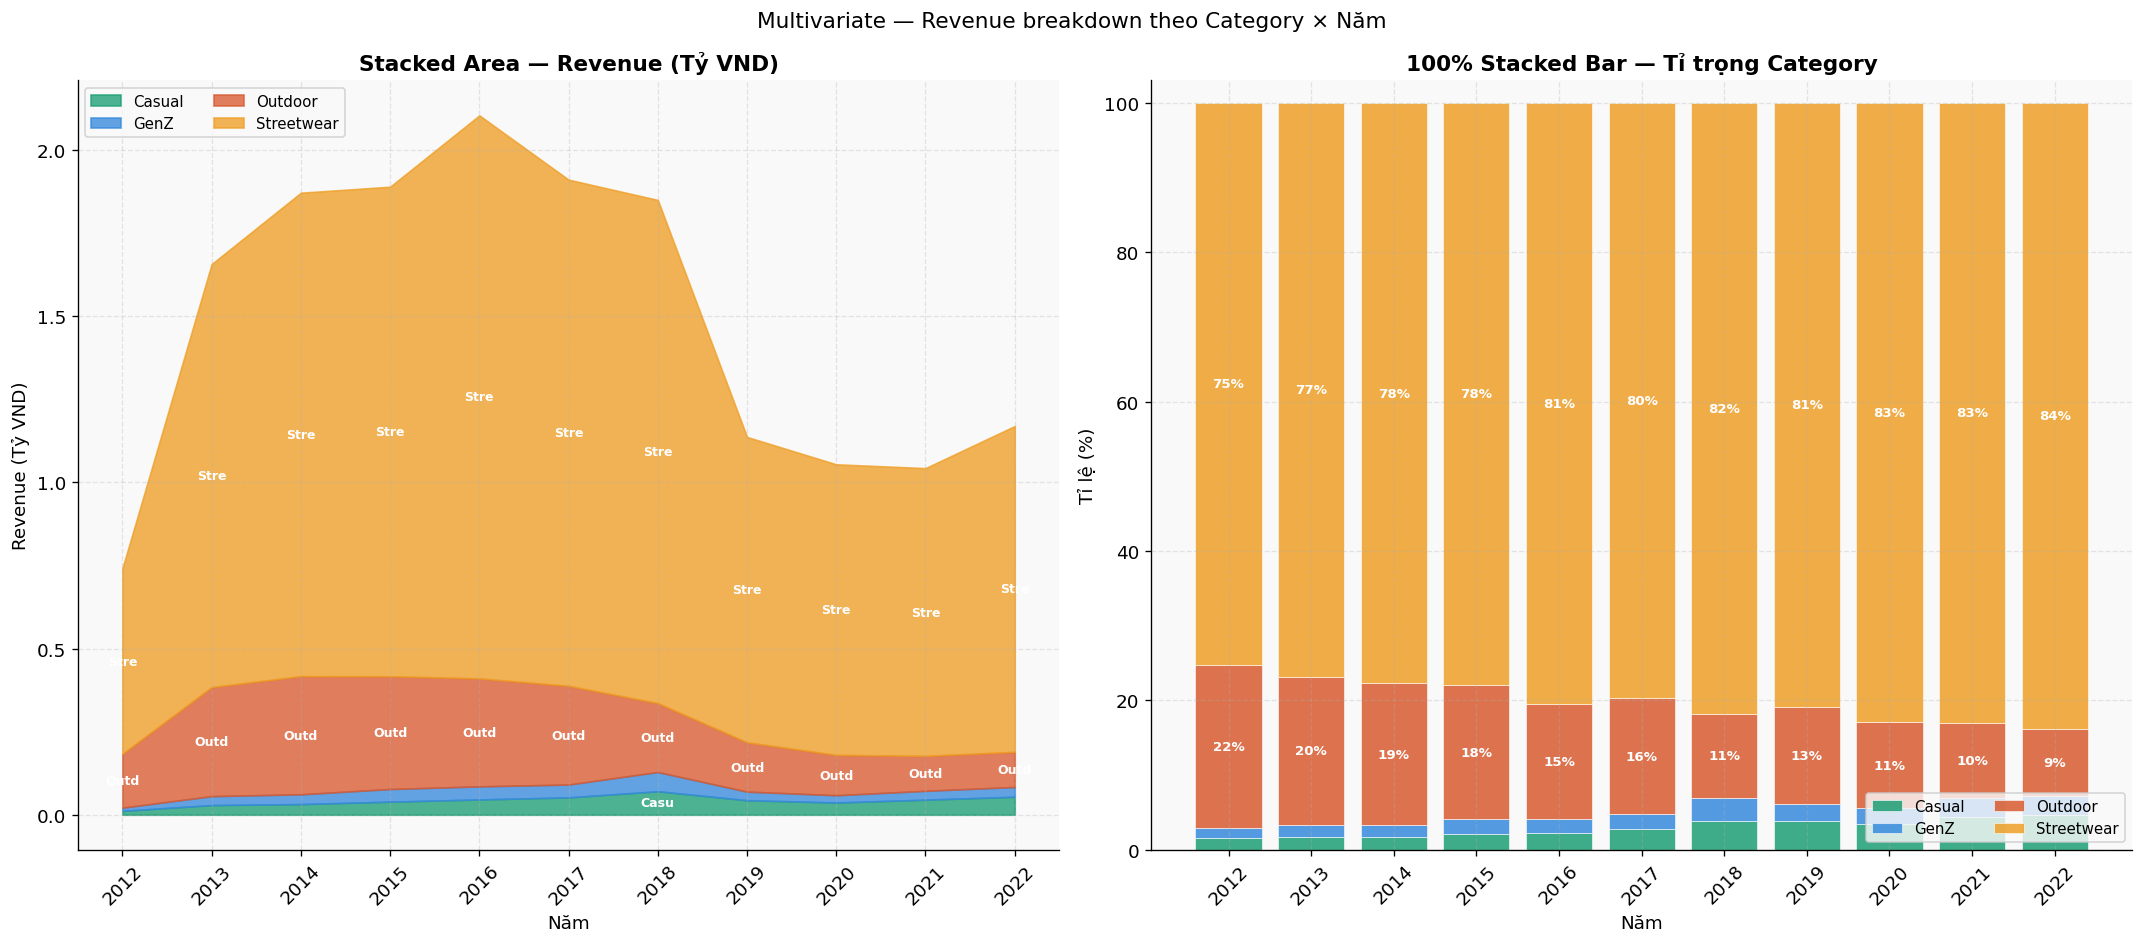
\includegraphics[width=\linewidth]{figures/eda/fig_multi_stacked.png}
  \caption{Revenue breakdown: Streetwear từ 75\% (2012) lên 84\% (2022)}
  \label{fig:stacked}
\end{subfigure}
\hfill
\begin{subfigure}[b]{0.49\linewidth}
  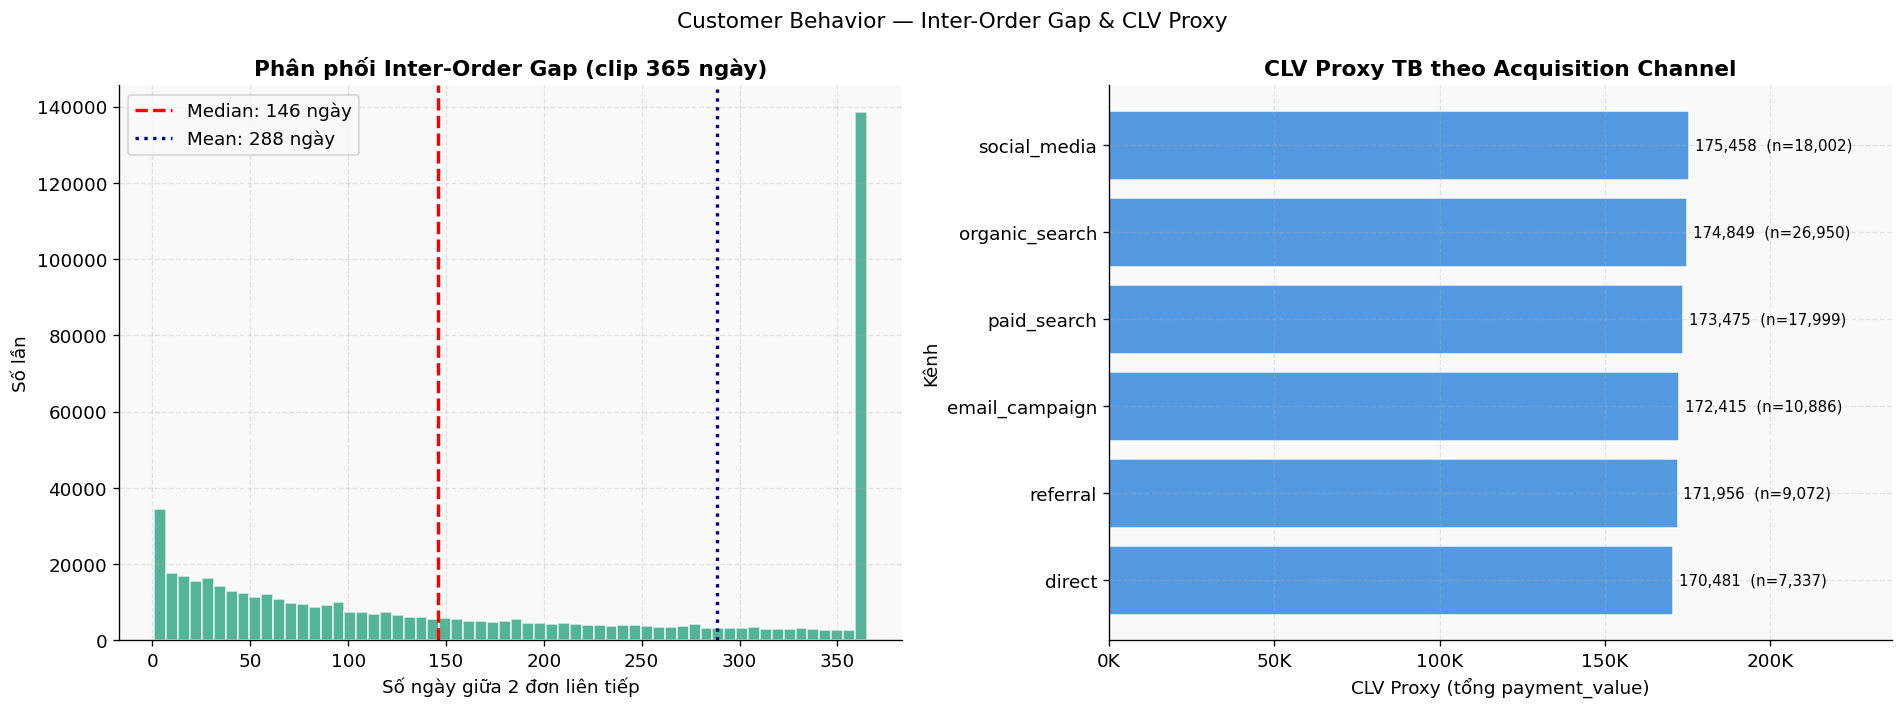
\includegraphics[width=\linewidth]{figures/eda/fig_clv_gap.png}
  \caption{CLV proxy \& inter-order gap: median = 146 ngày, mean = 288 ngày}
  \label{fig:clv}
\end{subfigure}
\caption{Cấu trúc doanh thu theo danh mục và hành vi mua lại của khách hàng.}
\end{figure}

\begin{figure}[h!]
\centering
\begin{subfigure}[b]{0.49\linewidth}
  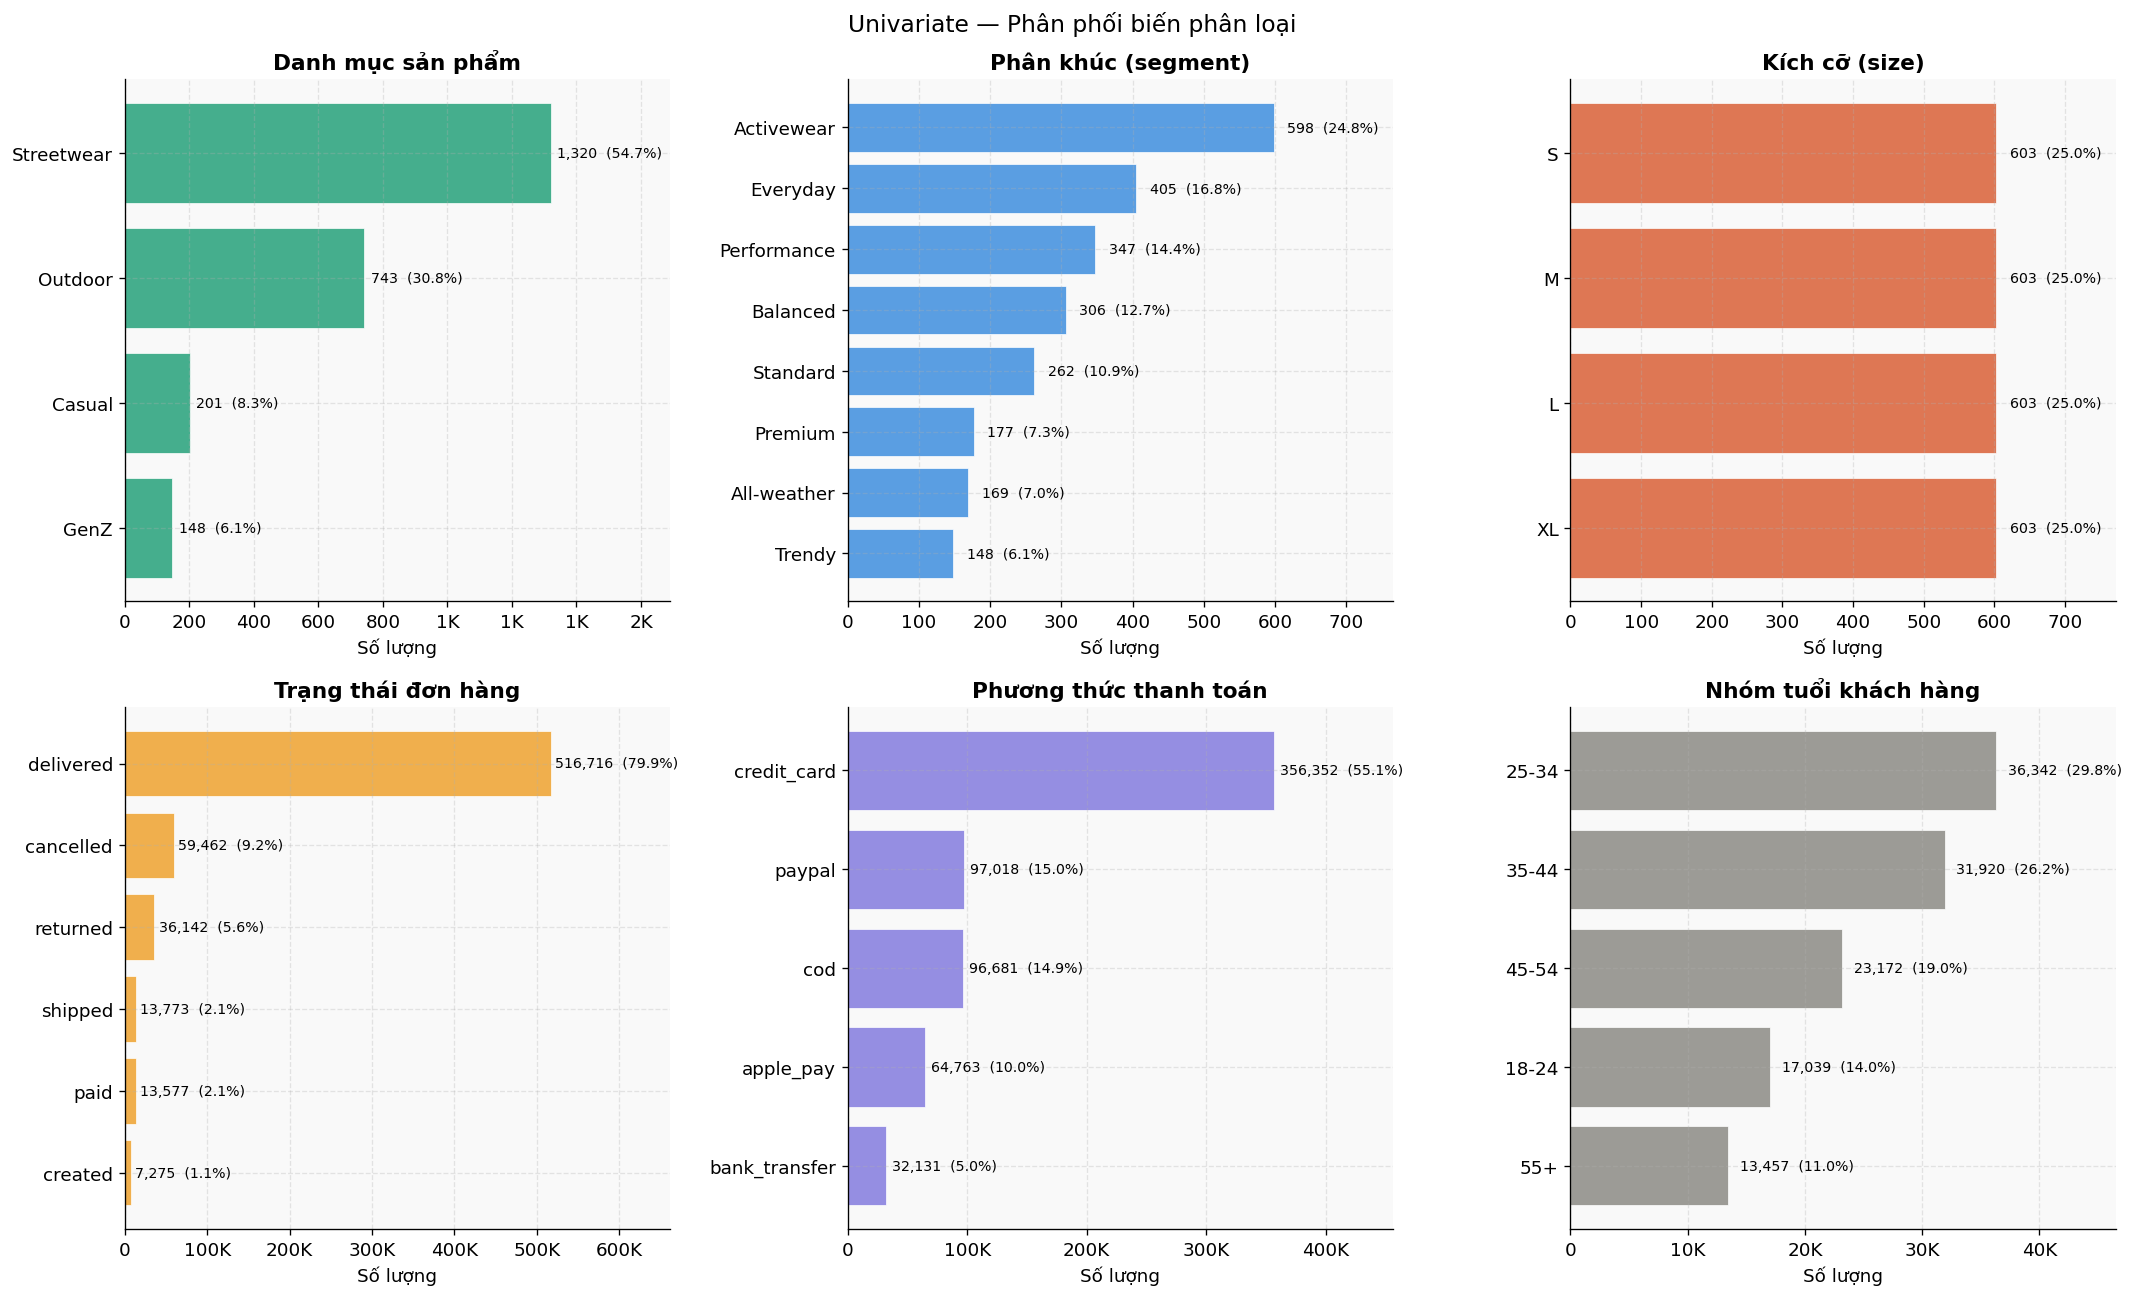
\includegraphics[width=\linewidth]{figures/eda/fig_uni_categorical.png}
  \caption{Phân phối biến phân loại: order status, payment, age group}
  \label{fig:uni_cat}
\end{subfigure}
\hfill
\begin{subfigure}[b]{0.49\linewidth}
  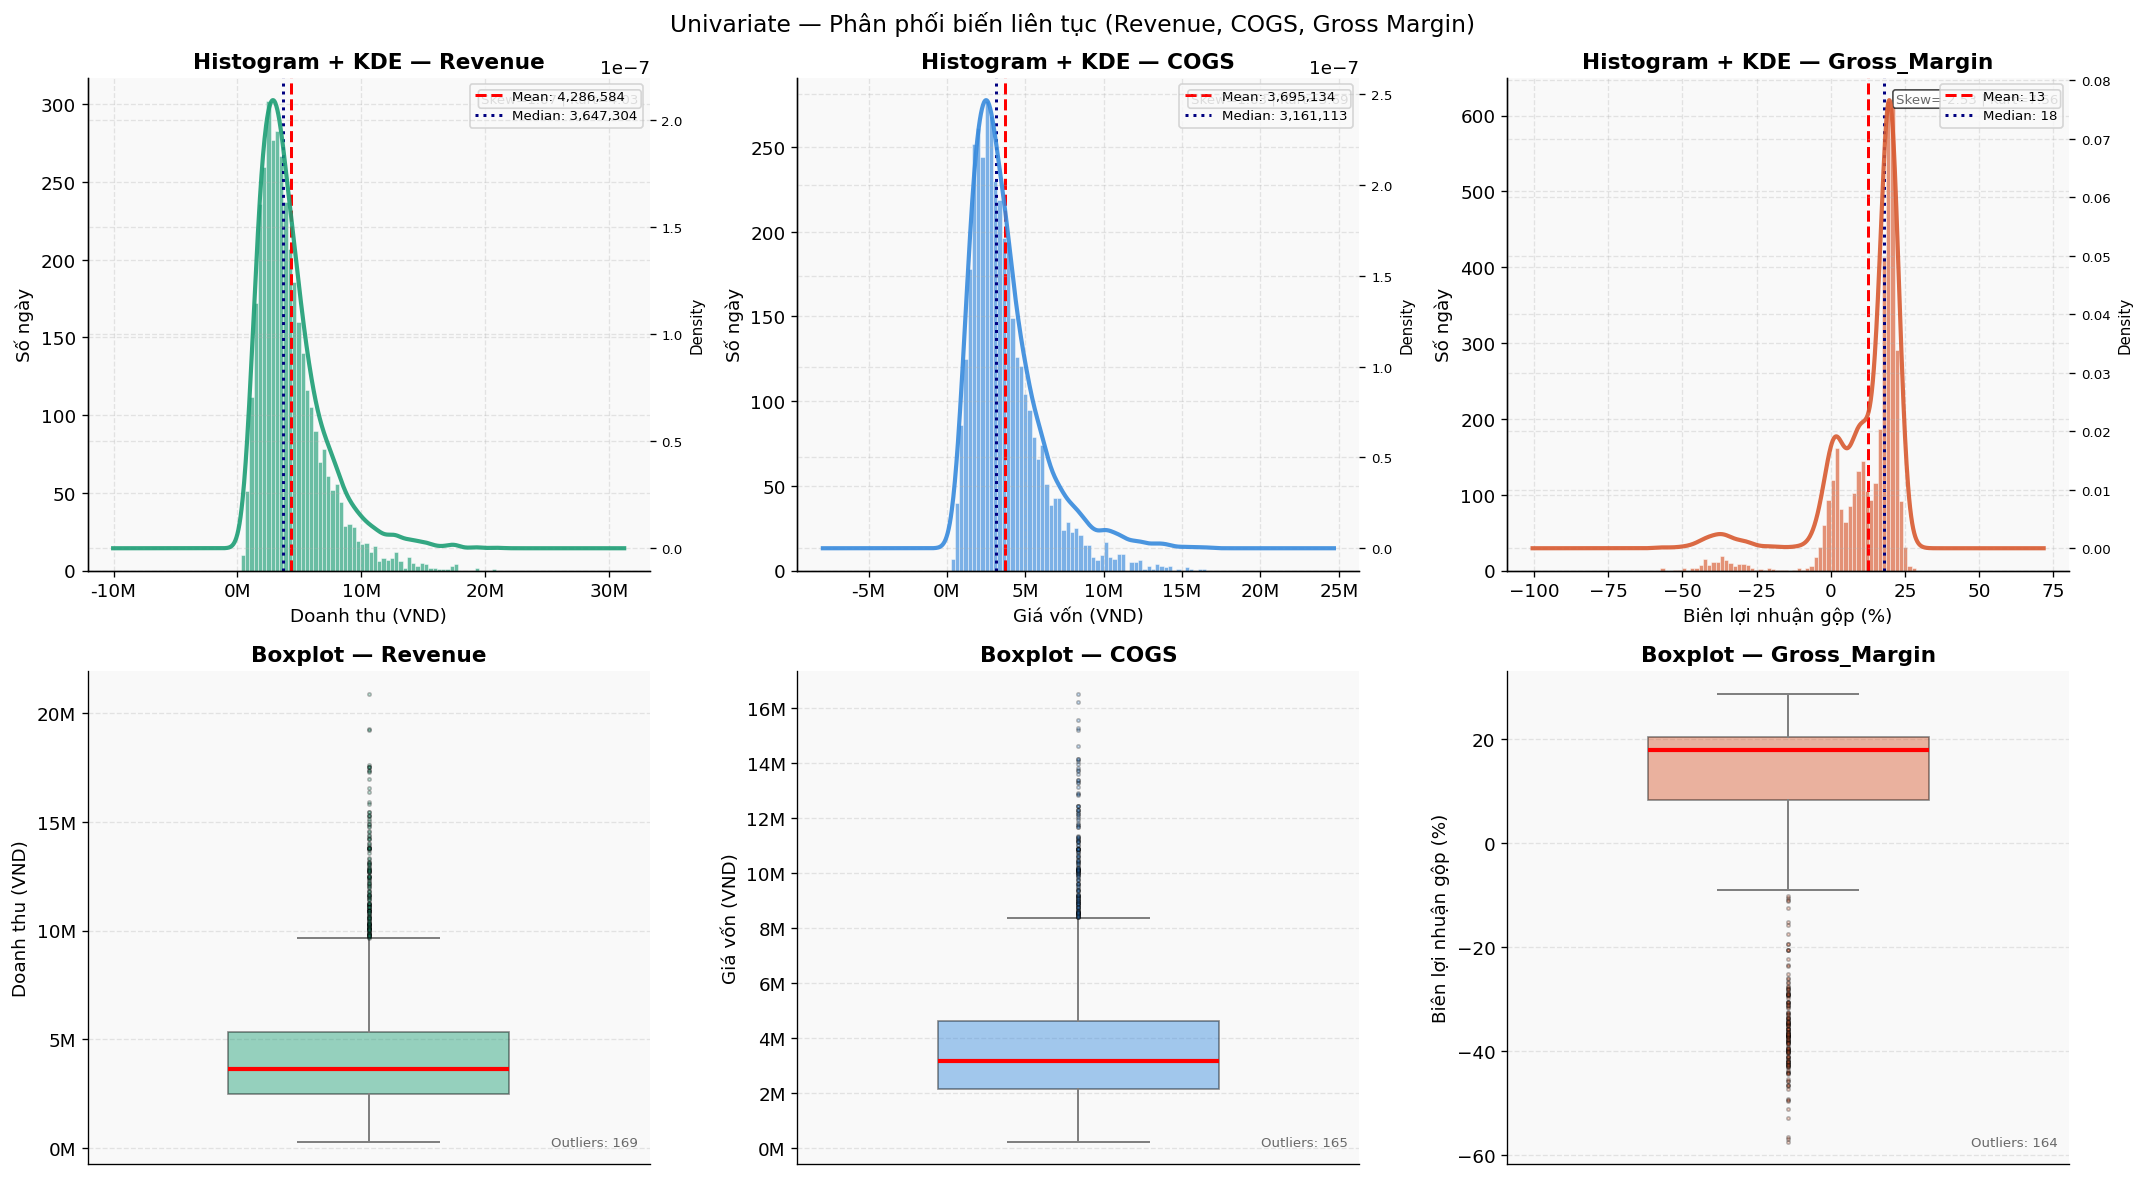
\includegraphics[width=\linewidth]{figures/eda/fig_uni_continuous.png}
  \caption{Phân phối Revenue/COGS/Margin: right-skewed, CV = 61\%}
  \label{fig:uni_cont}
\end{subfigure}
\caption{Phân tích đơn biến — biến phân loại và biến liên tục.}
\end{figure}

\begin{figure}[h!]
\centering
\begin{subfigure}[b]{0.49\linewidth}
  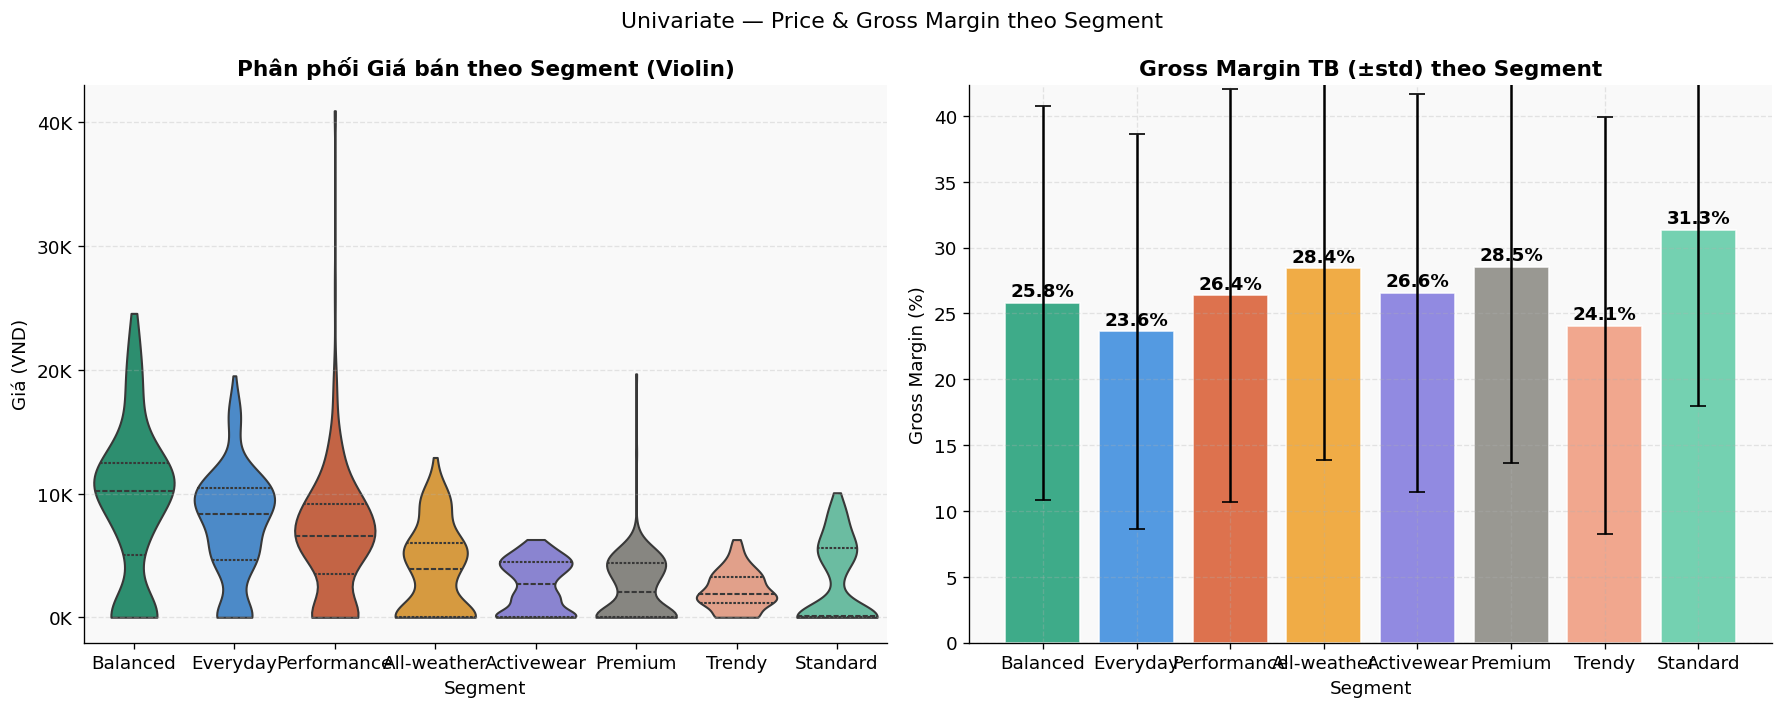
\includegraphics[width=\linewidth]{figures/eda/fig_uni_margin.png}
  \caption{Gross margin theo segment: Standard cao nhất (31,3\%), Everyday thấp nhất (23,6\%)}
  \label{fig:uni_margin}
\end{subfigure}
\hfill
\begin{subfigure}[b]{0.49\linewidth}
  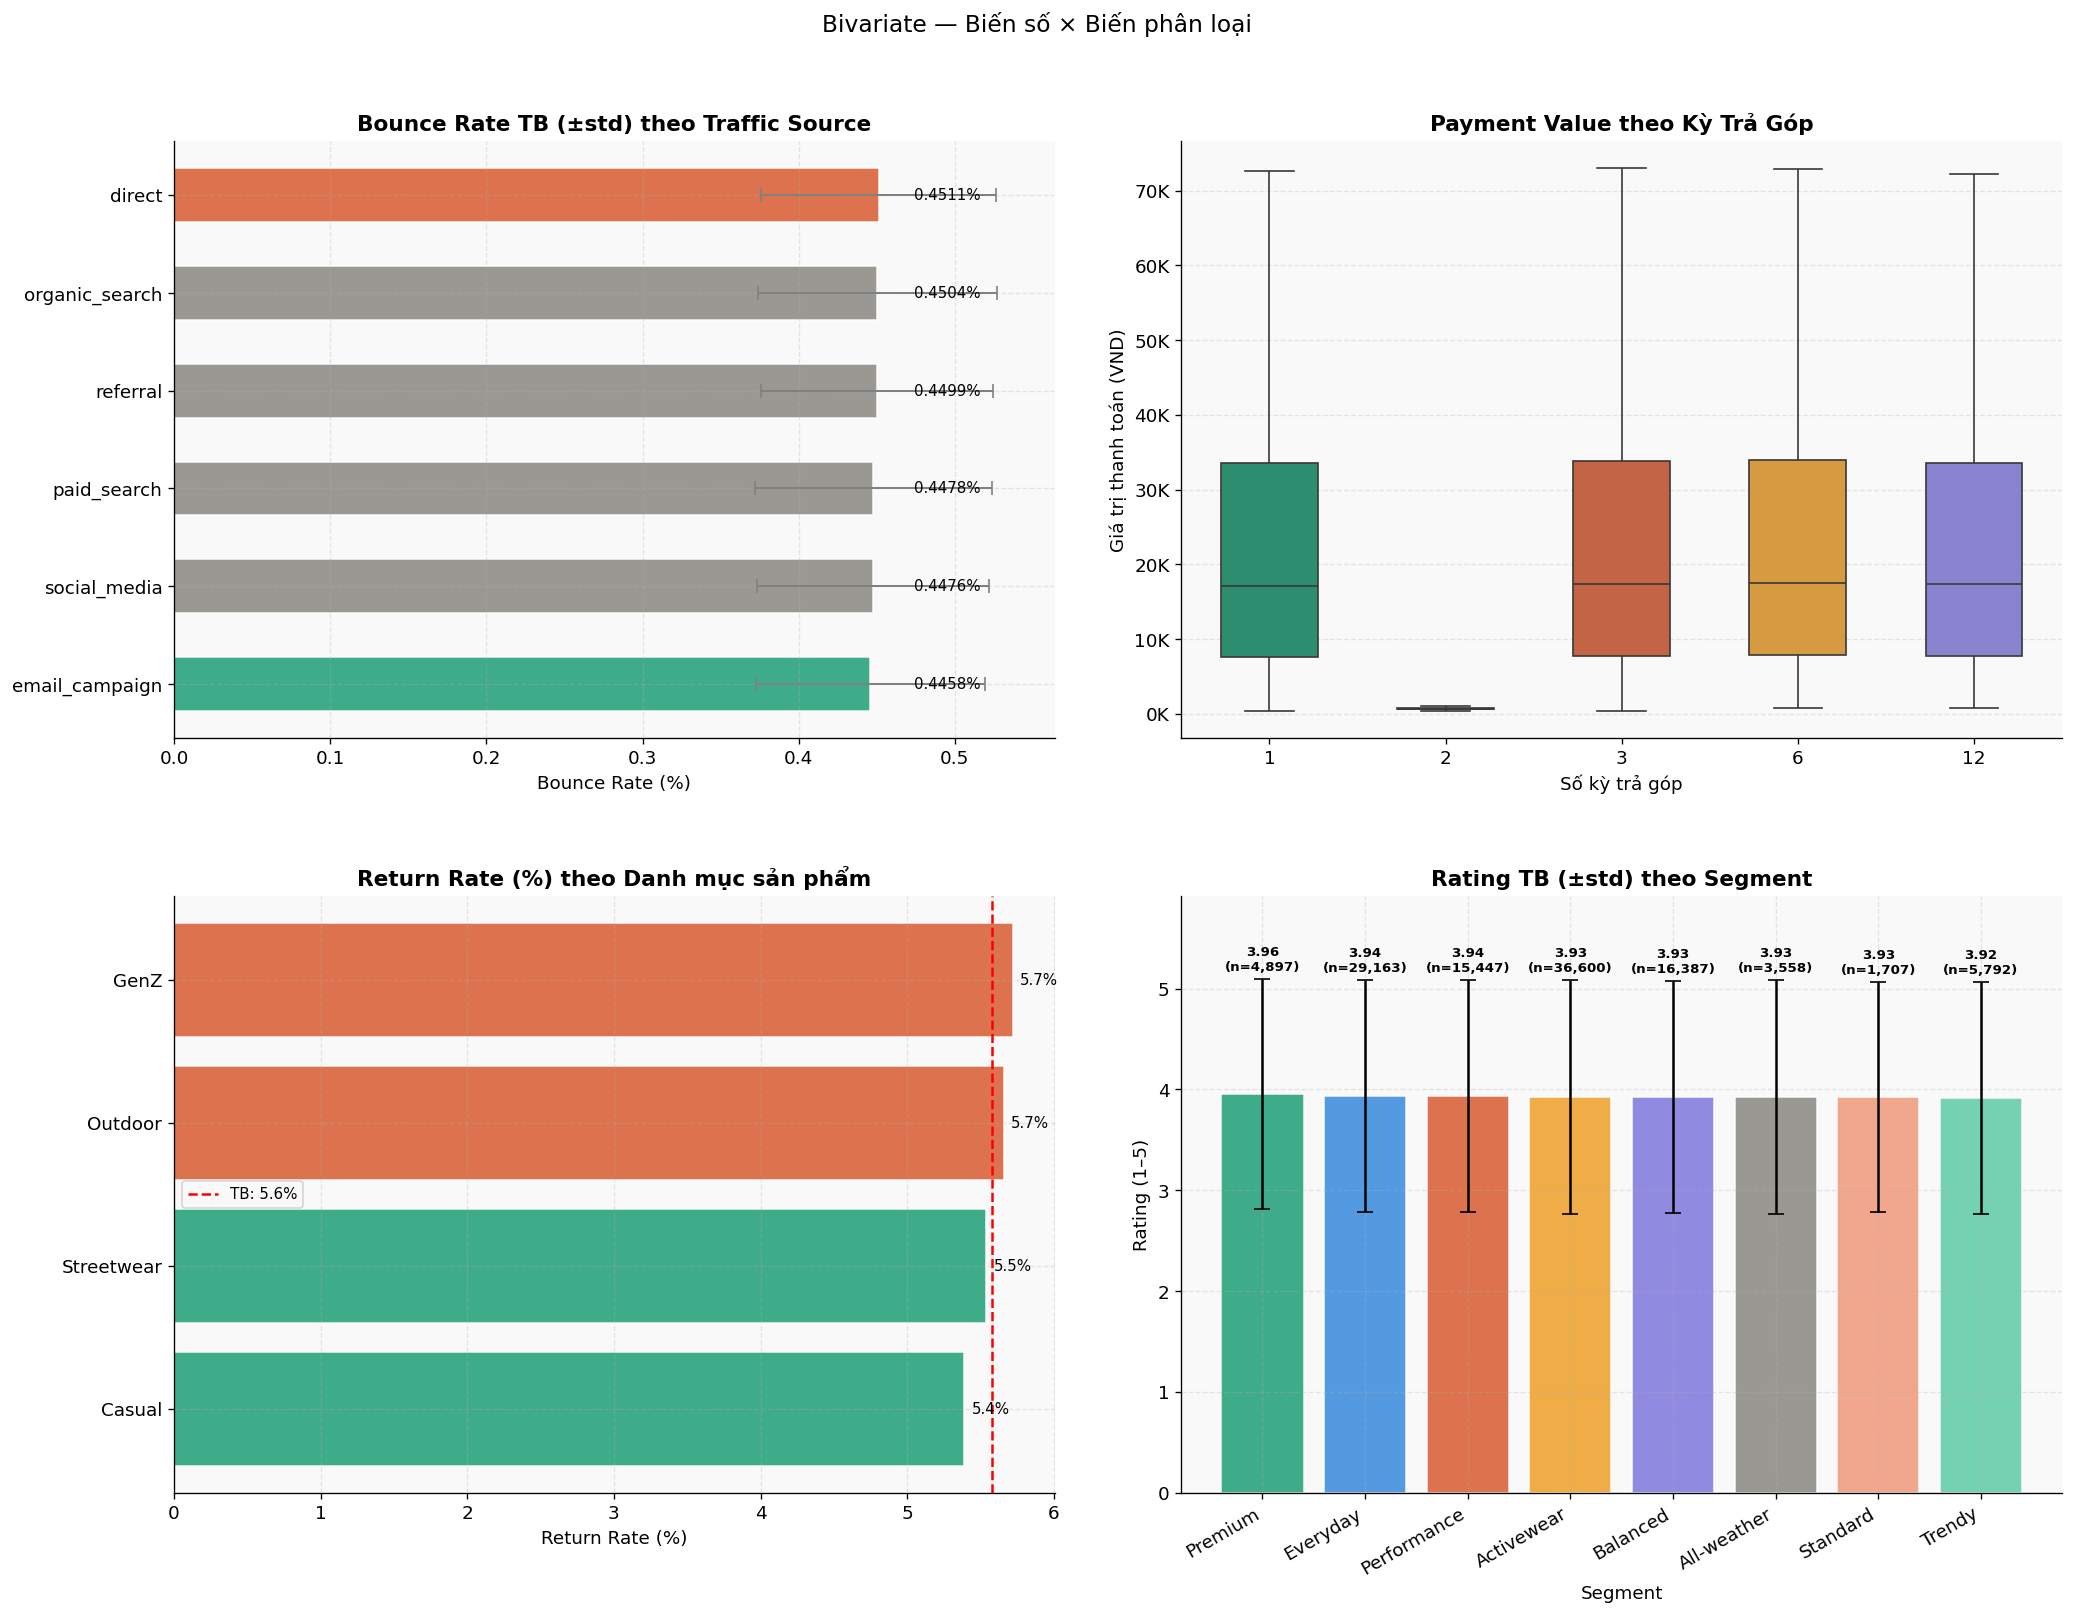
\includegraphics[width=\linewidth]{figures/eda/fig_bi_catnum.png}
  \caption{Bivariate: bounce rate đồng đều qua traffic sources; return rate cao nhất GenZ (5,7\%)}
  \label{fig:bicat}
\end{subfigure}
\caption{Phân tích margin theo phân khúc và bivariate tổng hợp.}
\end{figure}

% ===================================================================
\section{Phụ Lục B — Chi Tiết Pipeline Mô Hình}
% ===================================================================

\begin{figure}[h!]
\centering
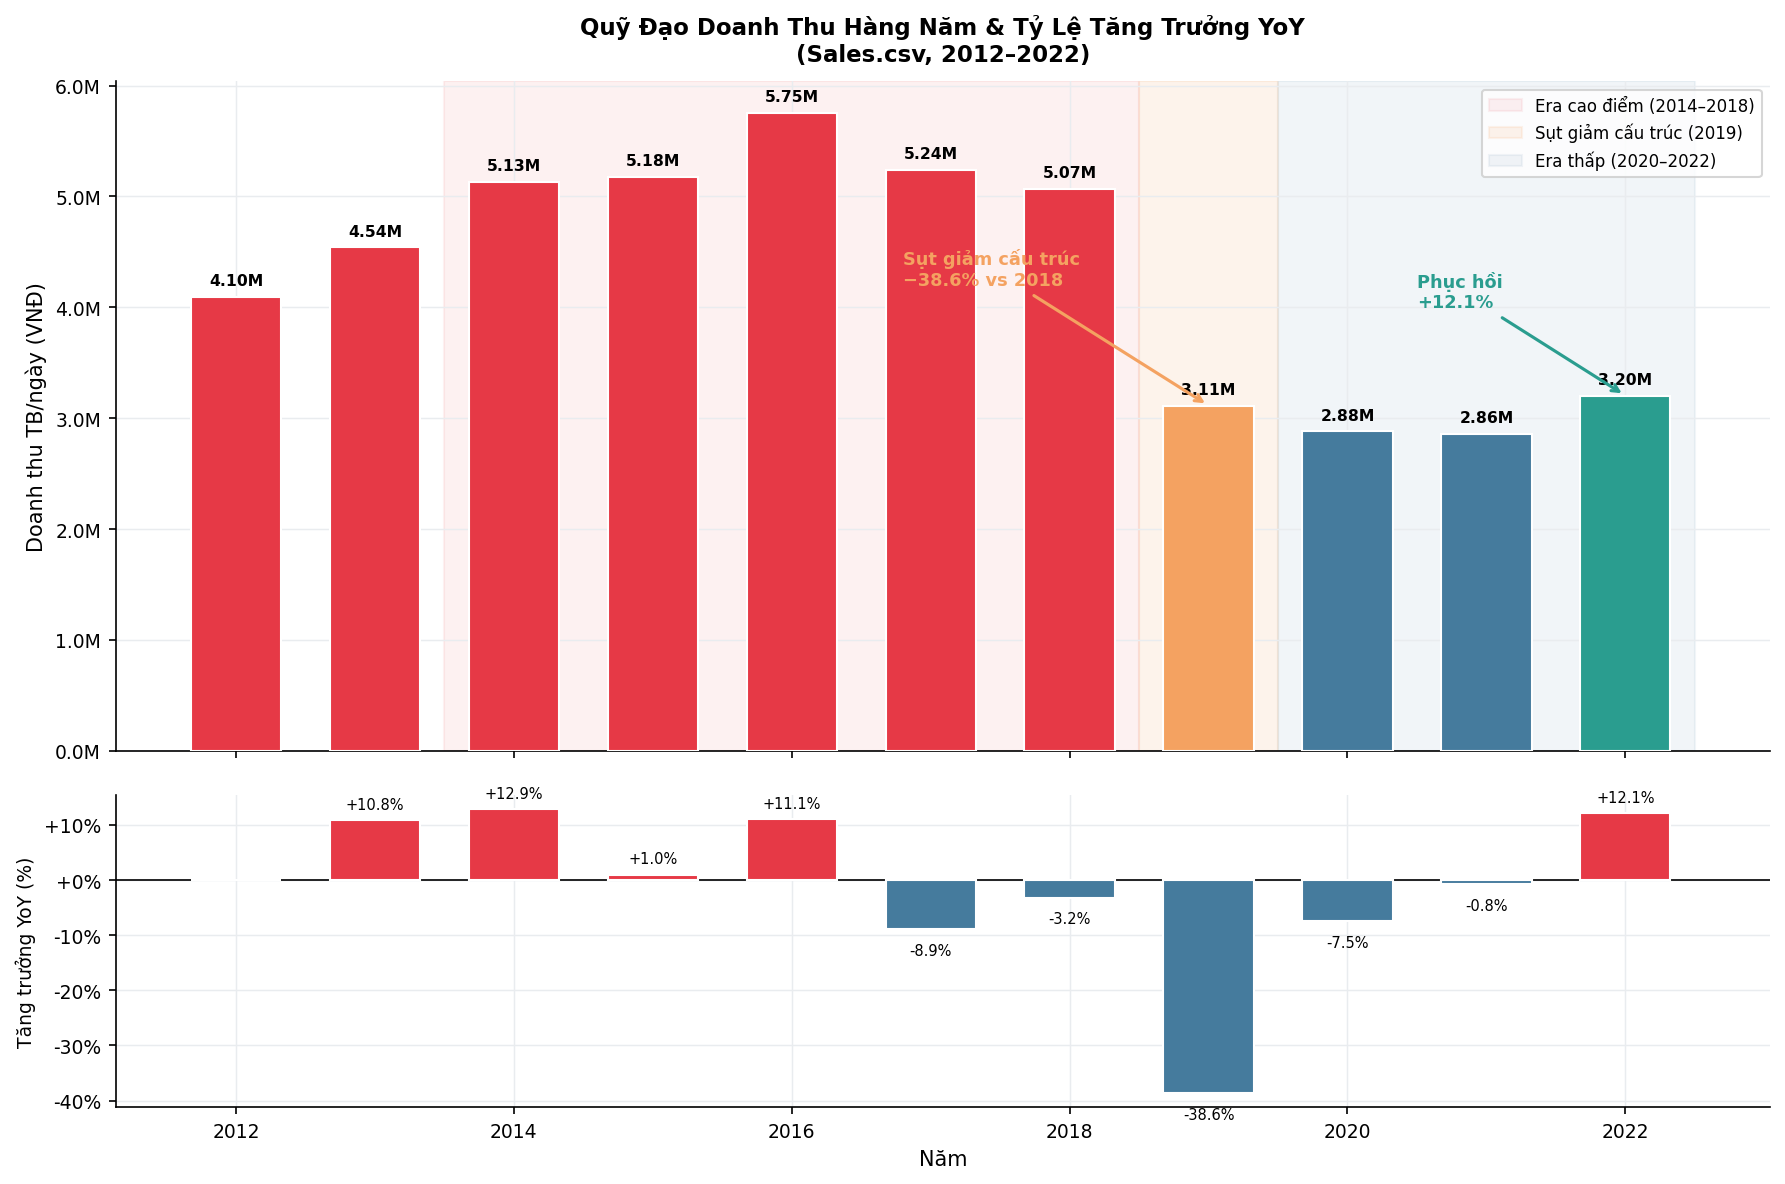
\includegraphics[width=\linewidth]{figures/modelling/fig1_annual_revenue_trajectory.png}
\caption{\textbf{Quỹ đạo doanh thu hàng năm.} Ba era rõ ràng: cao điểm 2014–2018 (5,13–5,75M), sụt giảm cấu trúc 2019 ($-38,6\%$), đáy phục hồi 2020–2022 (2,86–3,20M). Cơ sở cho CR calibration.}
\label{fig:annual}
\end{figure}

\begin{table}[h!]
\centering
\caption{COGS/Revenue margin theo Quý × Năm Lẻ/Chẵn (dữ liệu $\geq$2020) — cơ sở công thức CC}
\label{tab:margin_qparity}
\small
\begin{tabular}{lcccc}
\toprule
& \textbf{Q1} & \textbf{Q2} & \textbf{Q3} & \textbf{Q4} \\
\midrule
Năm lẻ  & 0,8301 & 0,8306 & \textbf{1,0570} & 0,8917 \\
Năm chẵn & 0,8449 & 0,8404 & 0,8716          & 0,8897 \\
\bottomrule
\end{tabular}
\end{table}

\begin{figure}[h!]
\centering
\begin{subfigure}[b]{0.49\linewidth}
  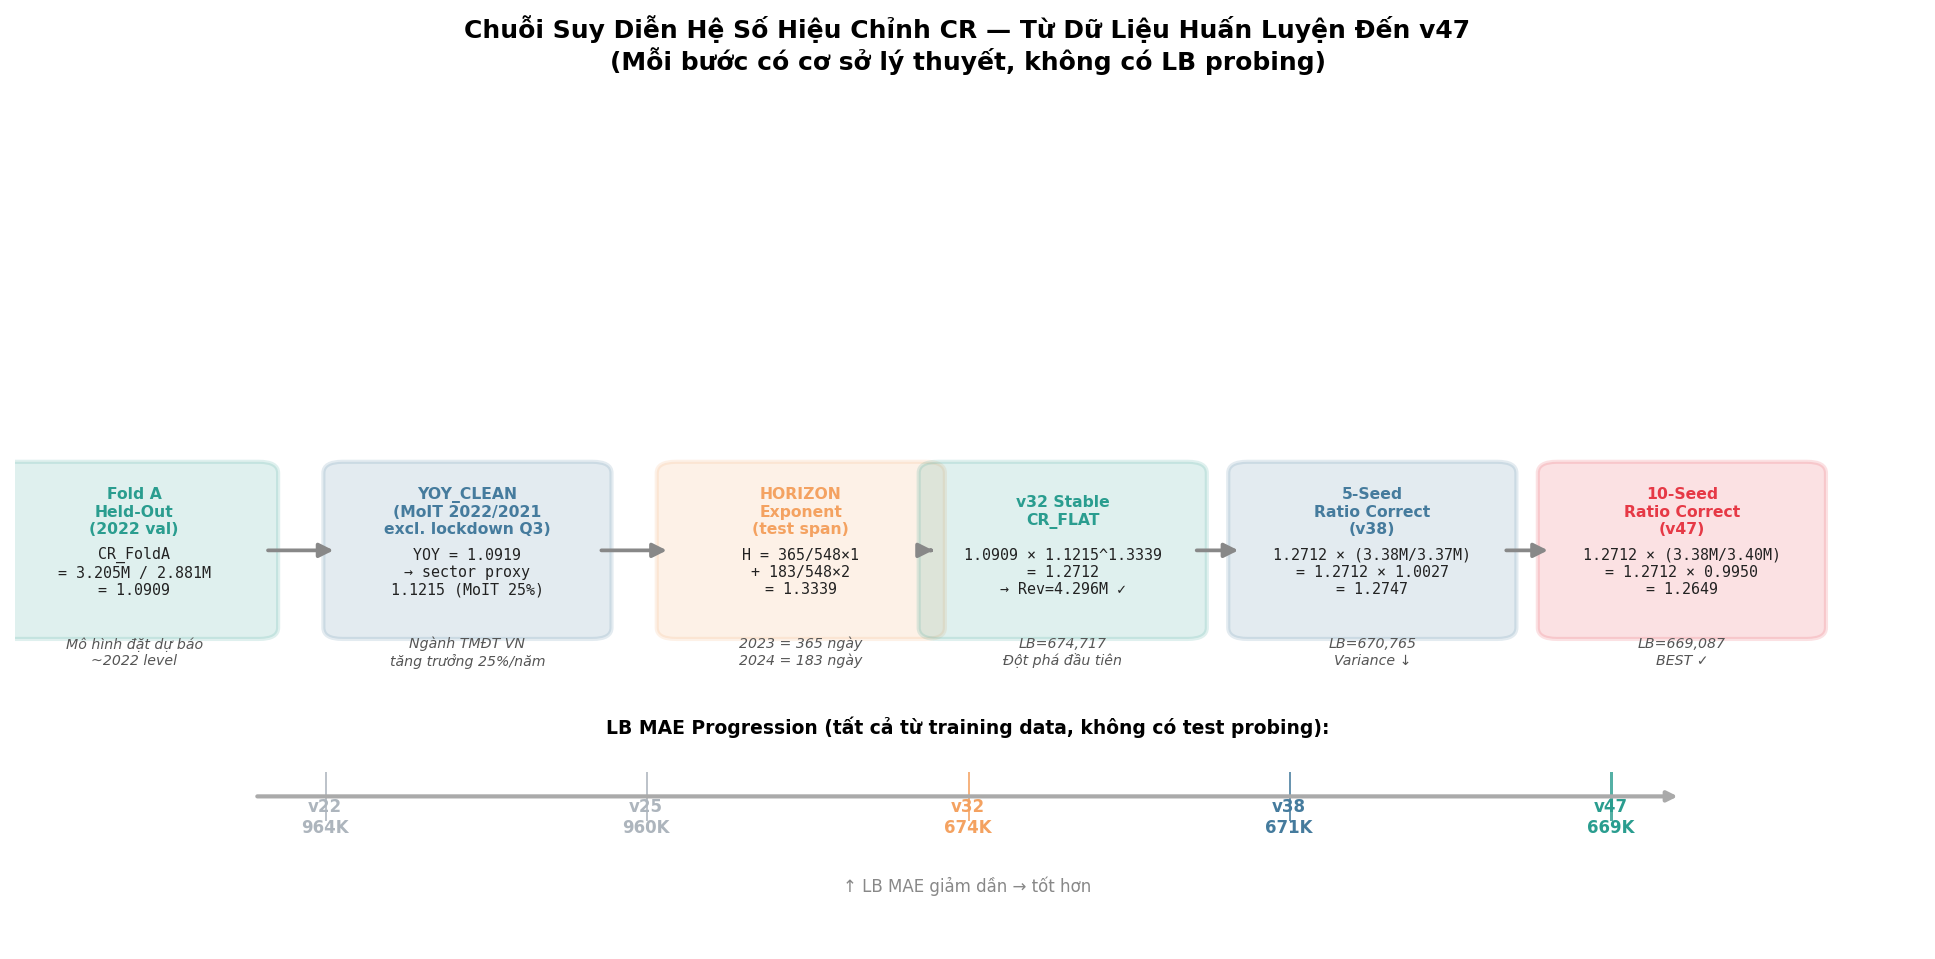
\includegraphics[width=\linewidth]{figures/modelling/fig4_cr_derivation_chain.png}
  \caption{Chuỗi suy diễn CR từ Fold A đến v47}
  \label{fig:cr_chain}
\end{subfigure}
\hfill
\begin{subfigure}[b]{0.49\linewidth}
  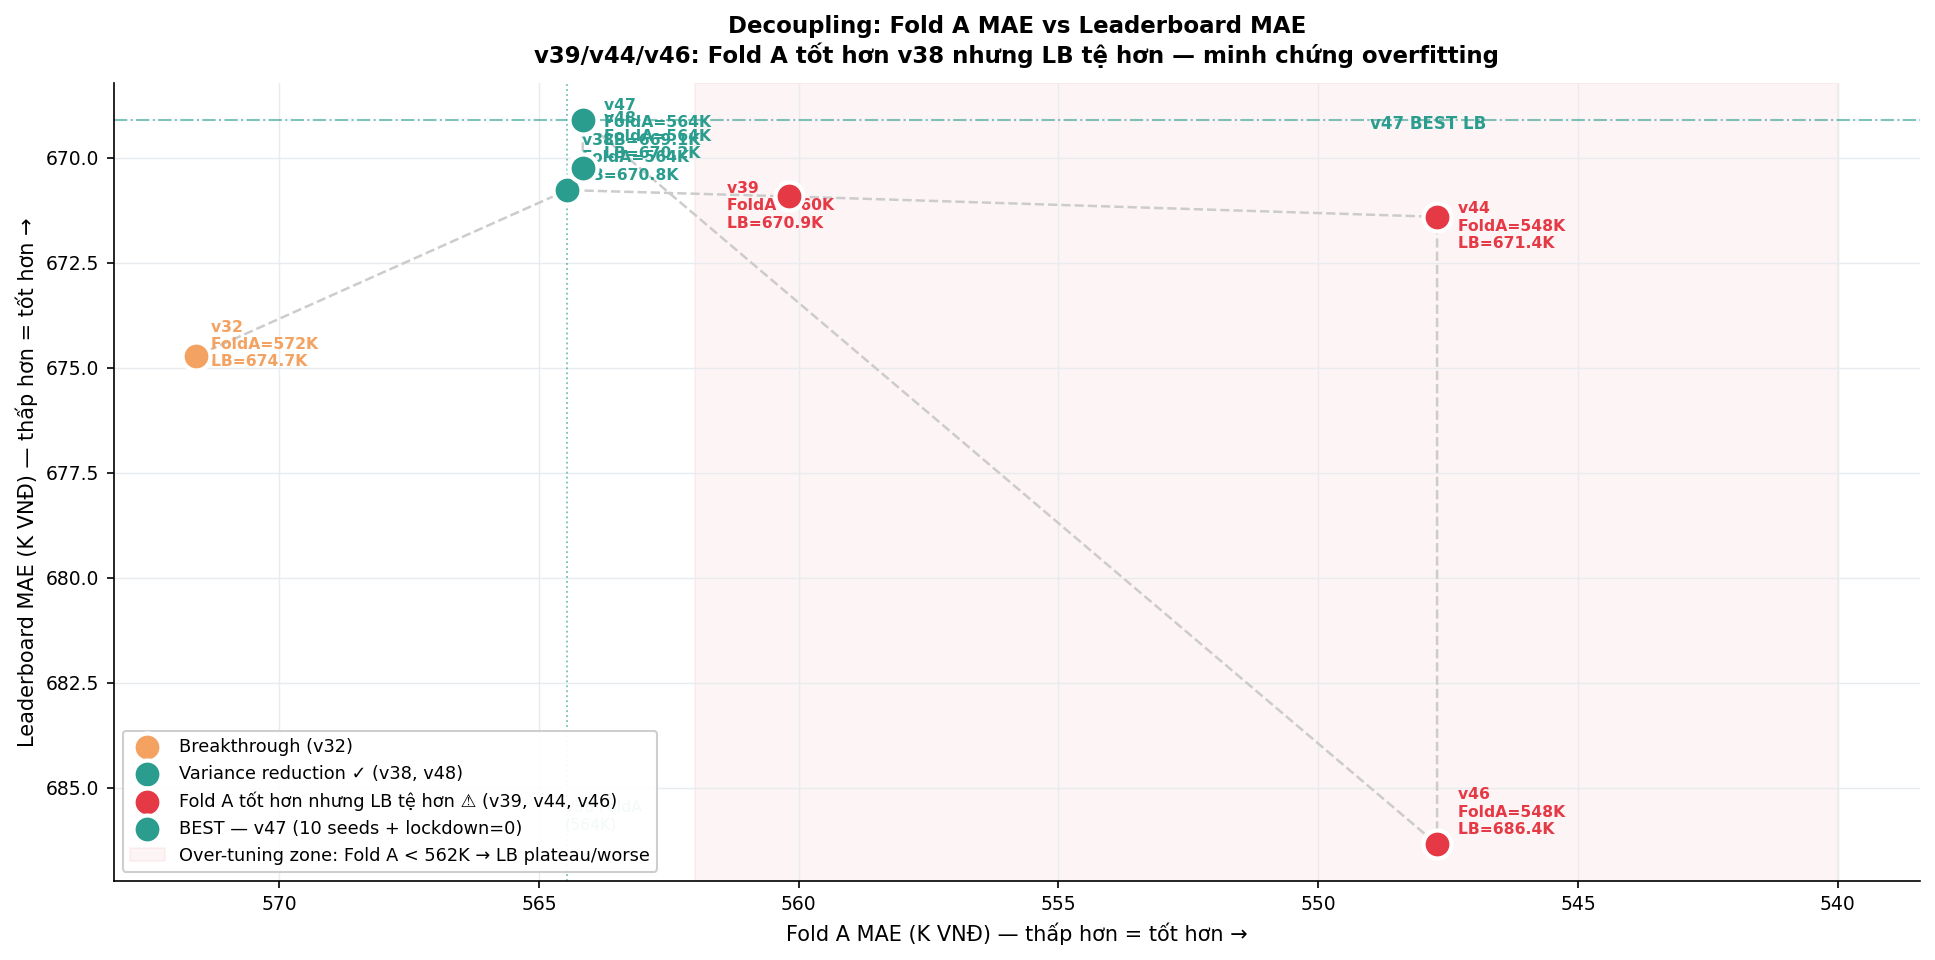
\includegraphics[width=\linewidth]{figures/modelling/fig5_folda_vs_lb_decoupling.png}
  \caption{Decoupling: Fold A tốt hơn không đảm bảo LB tốt hơn}
  \label{fig:decoupling}
\end{subfigure}
\caption{Chuỗi suy diễn CR và hiện tượng decoupling Fold A vs LB.}
\end{figure}

\begin{figure}[h!]
\centering
\begin{subfigure}[b]{0.49\linewidth}
  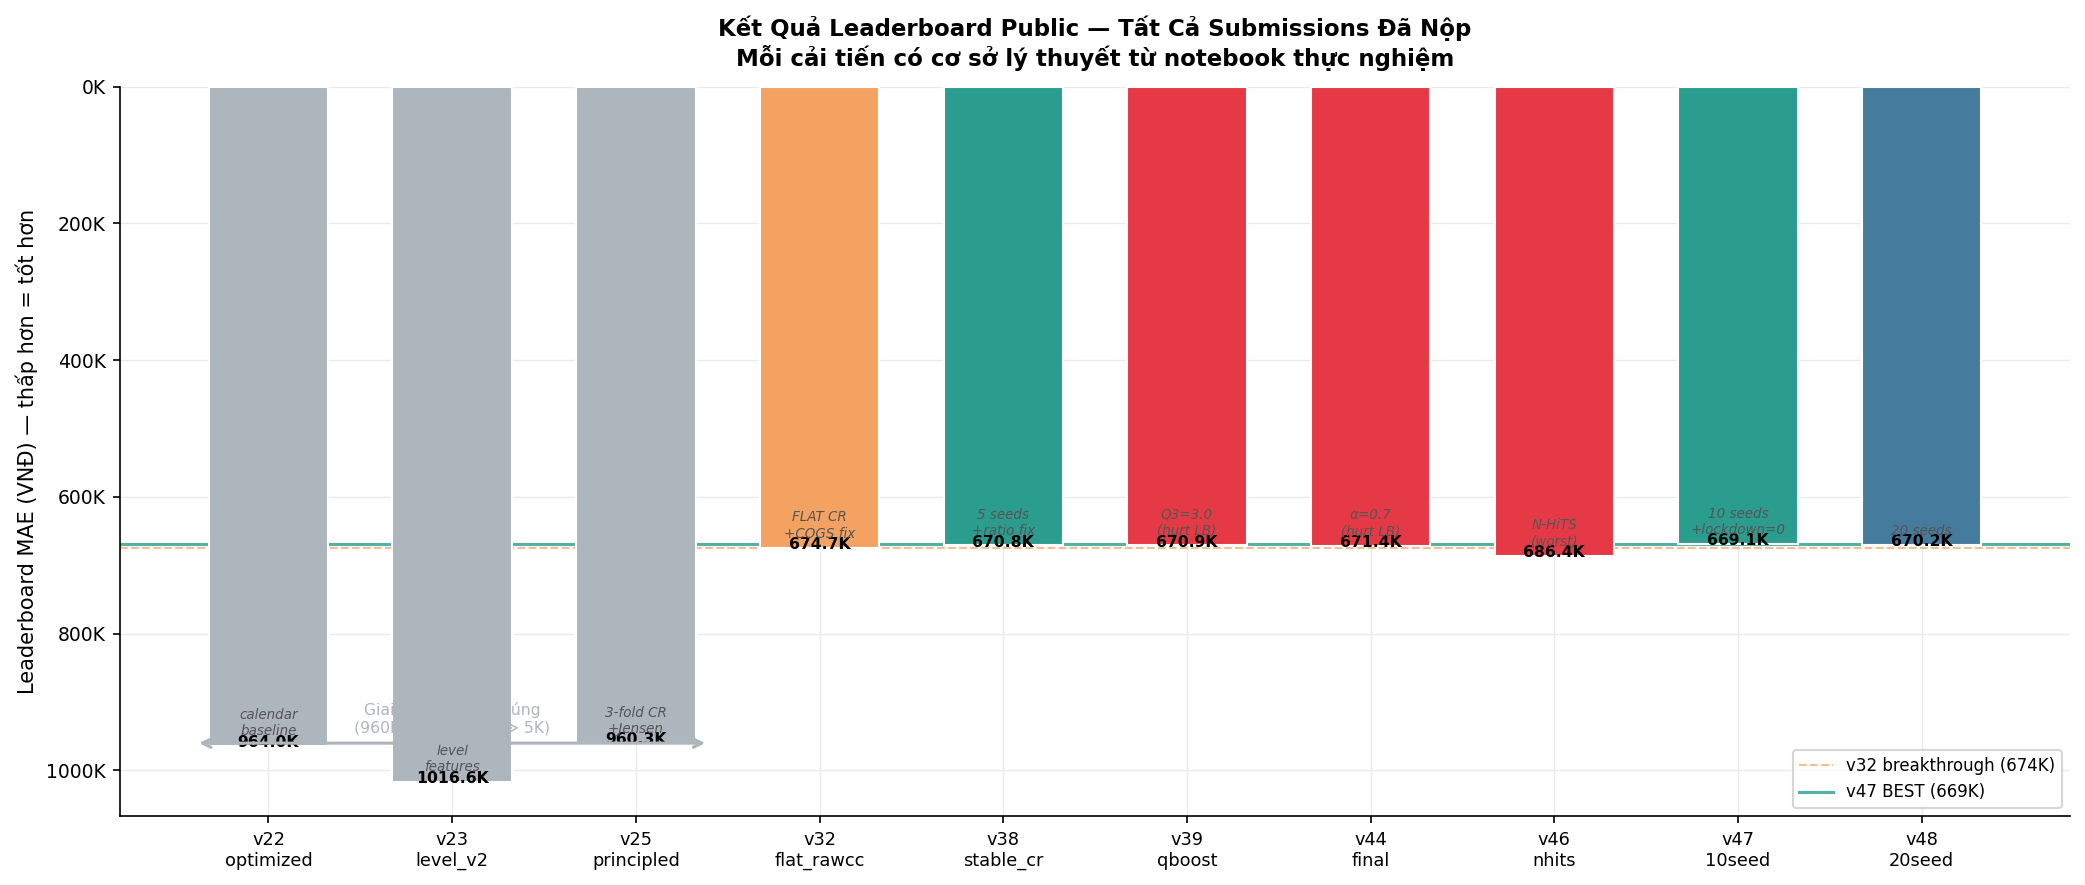
\includegraphics[width=\linewidth]{figures/modelling/fig7_leaderboard_progression.png}
  \caption{Tiến trình LB MAE qua các submissions}
  \label{fig:lb_prog}
\end{subfigure}
\hfill
\begin{subfigure}[b]{0.49\linewidth}
  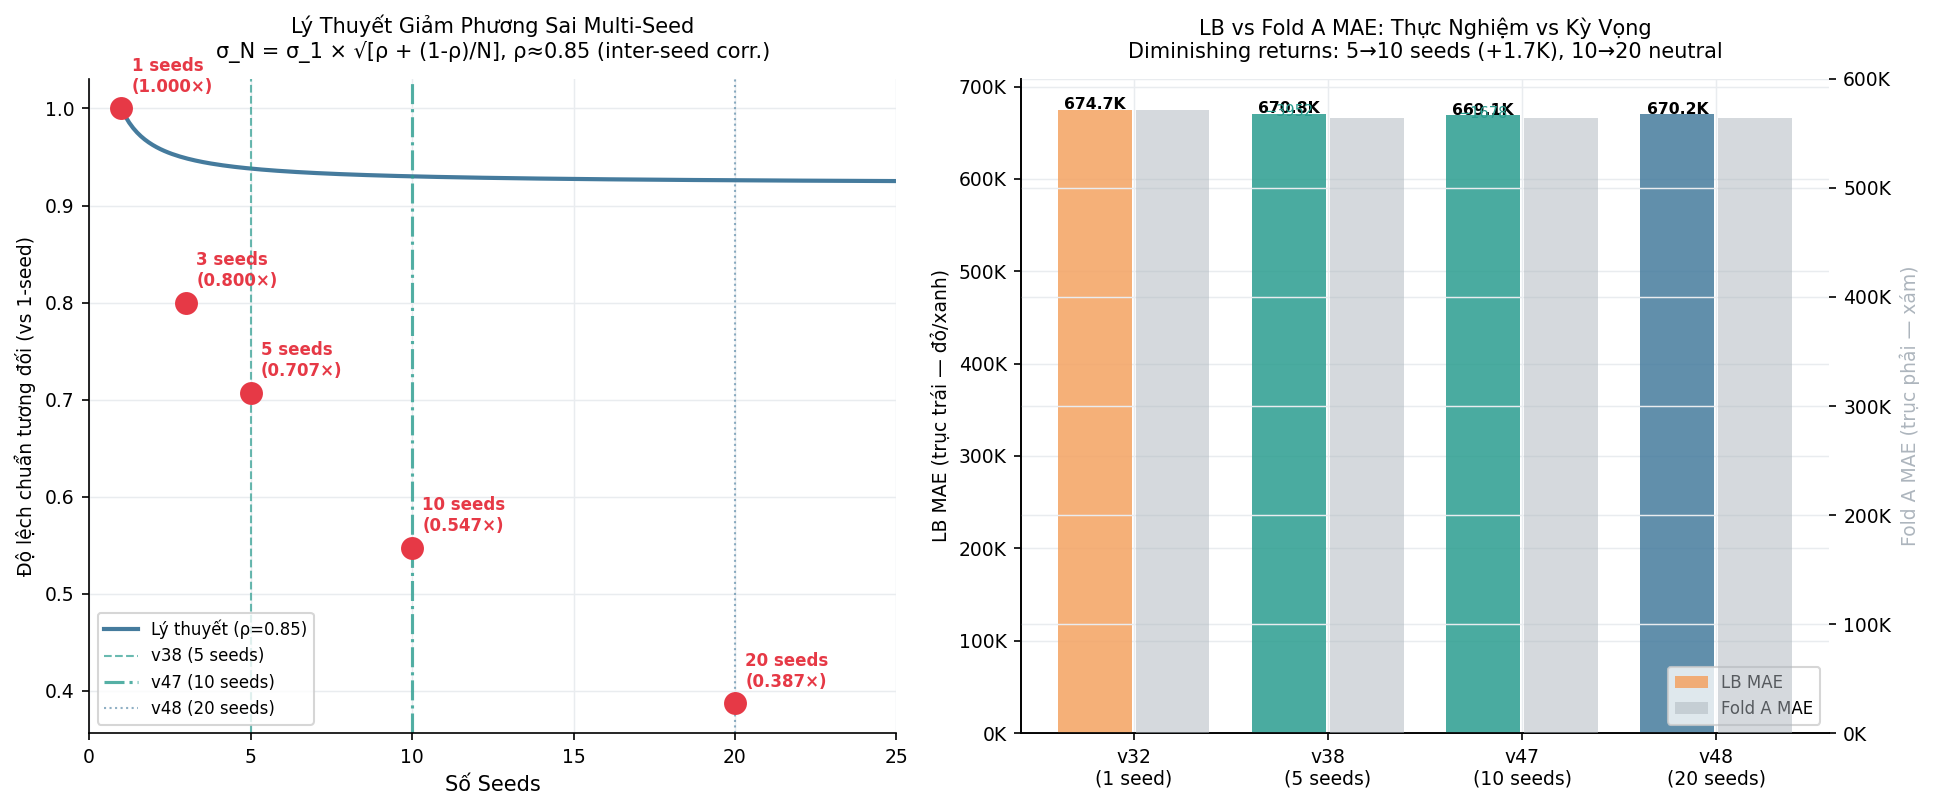
\includegraphics[width=\linewidth]{figures/modelling/fig8_seed_variance_reduction.png}
  \caption{Lý thuyết và thực nghiệm giảm phương sai multi-seed}
  \label{fig:seed_var}
\end{subfigure}
\caption{Kết quả LB và hiệu quả giảm phương sai multi-seed.}
\end{figure}

\begin{figure}[h!]
\centering
\begin{subfigure}[b]{0.49\linewidth}
  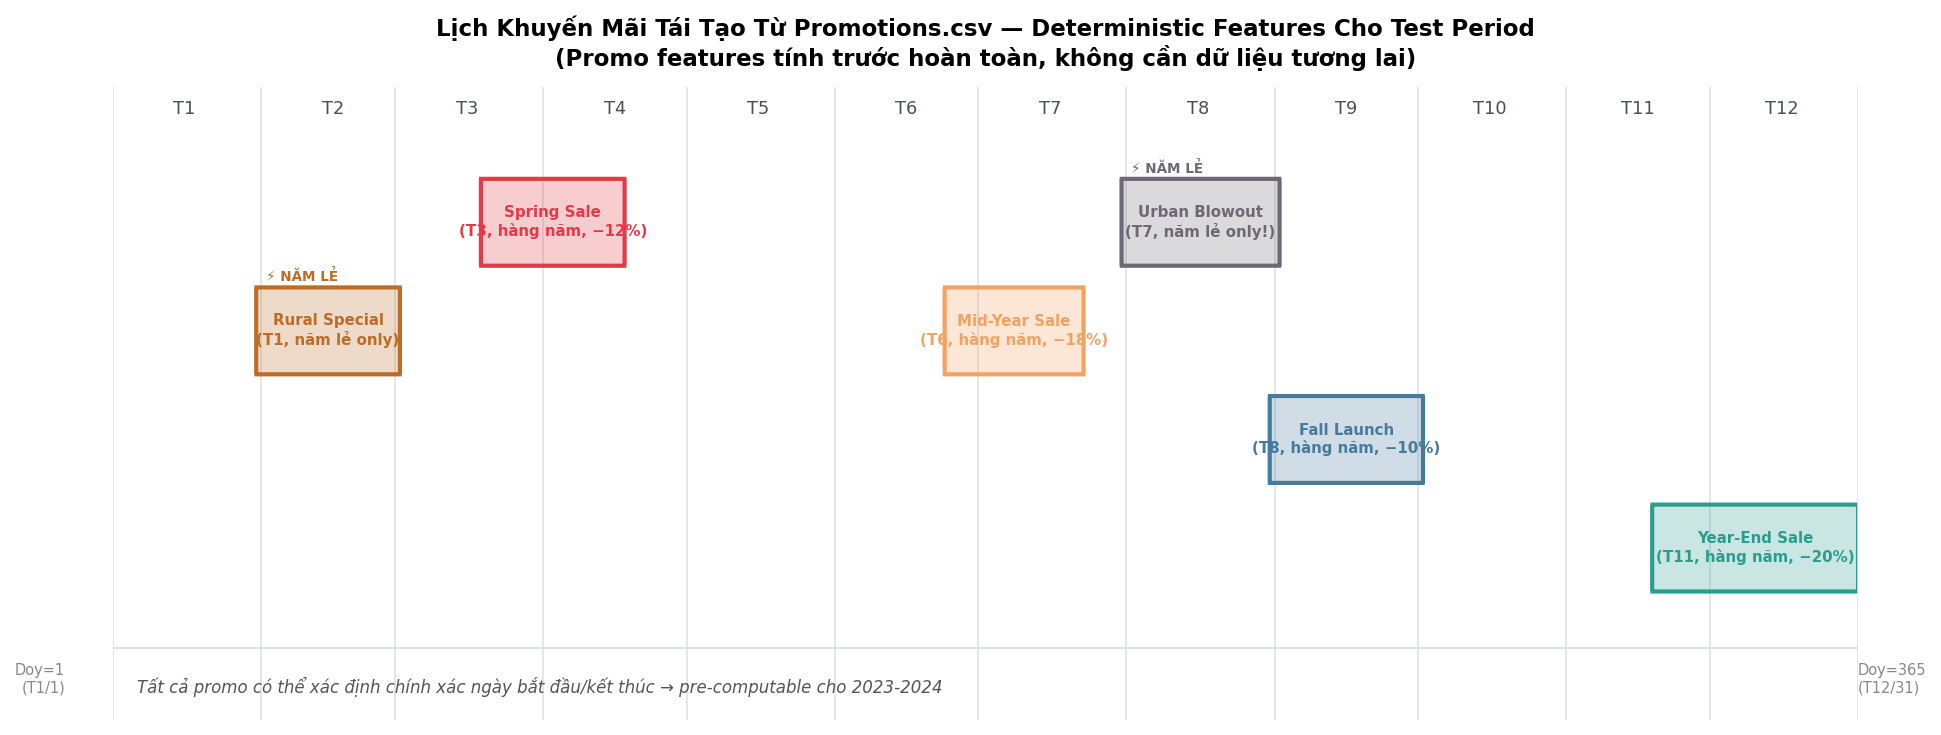
\includegraphics[width=\linewidth]{figures/modelling/fig9_promo_schedule.png}
  \caption{Lịch 6 chiến dịch khuyến mãi — deterministic, pre-computable}
  \label{fig:promo}
\end{subfigure}
\hfill
\begin{subfigure}[b]{0.49\linewidth}
  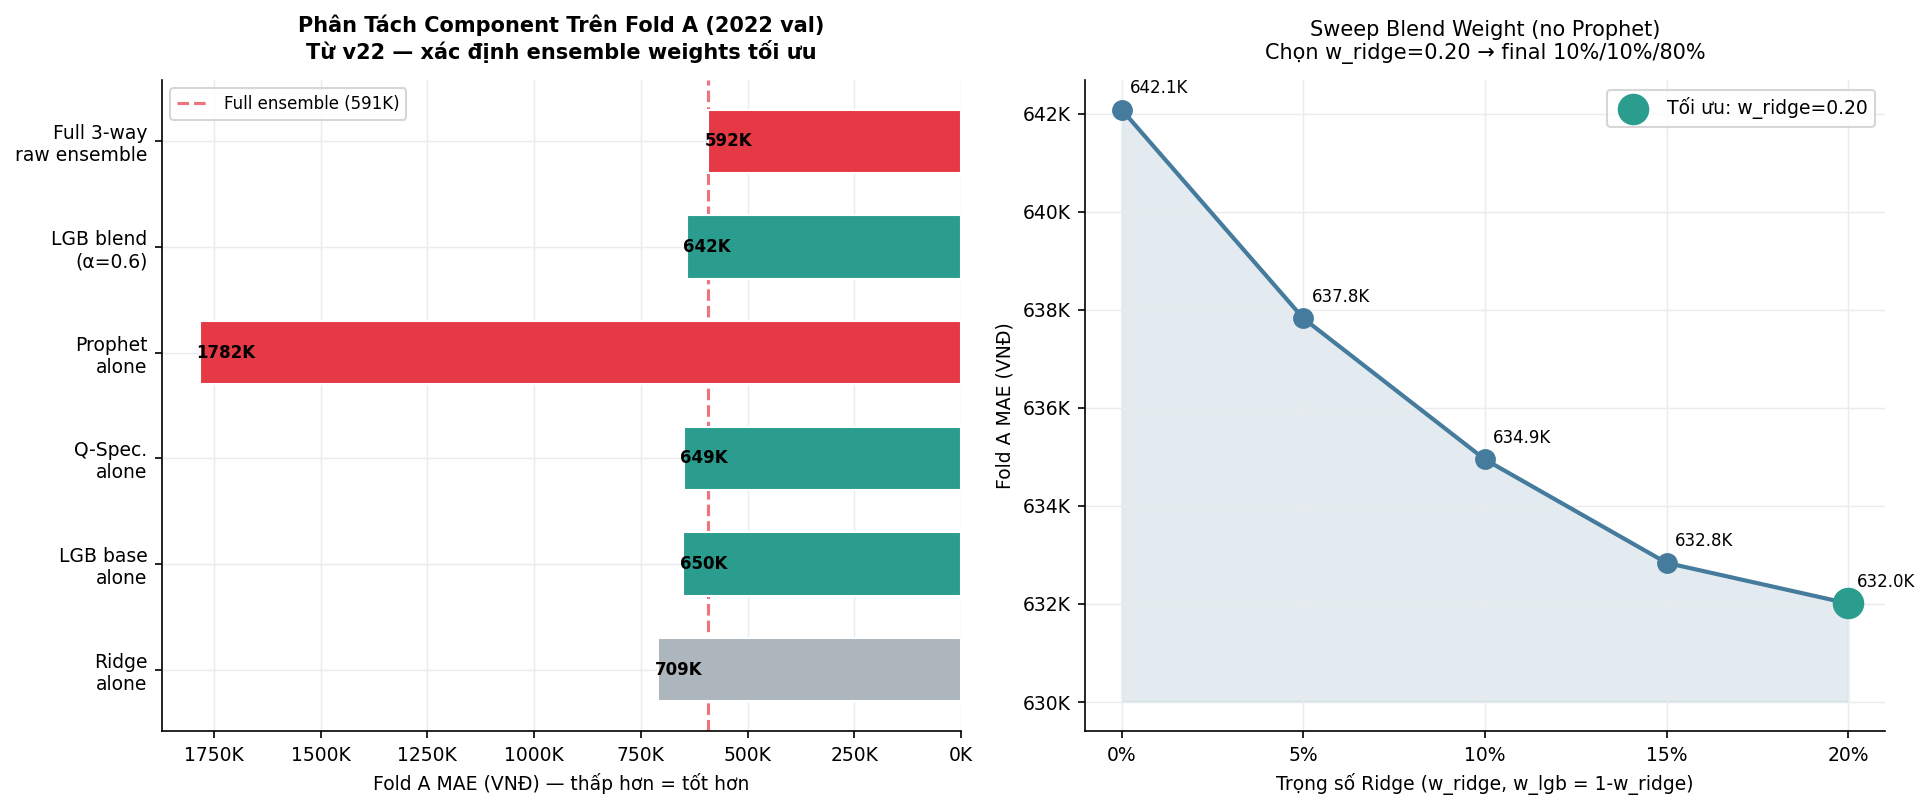
\includegraphics[width=\linewidth]{figures/modelling/fig10_component_analysis.png}
  \caption{Phân tích đóng góp từng component và sweep blend weight}
  \label{fig:component}
\end{subfigure}
\caption{Lịch khuyến mãi và phân tích component ensemble.}
\end{figure}

\begin{figure}[h!]
\centering
\begin{subfigure}[b]{0.49\linewidth}
  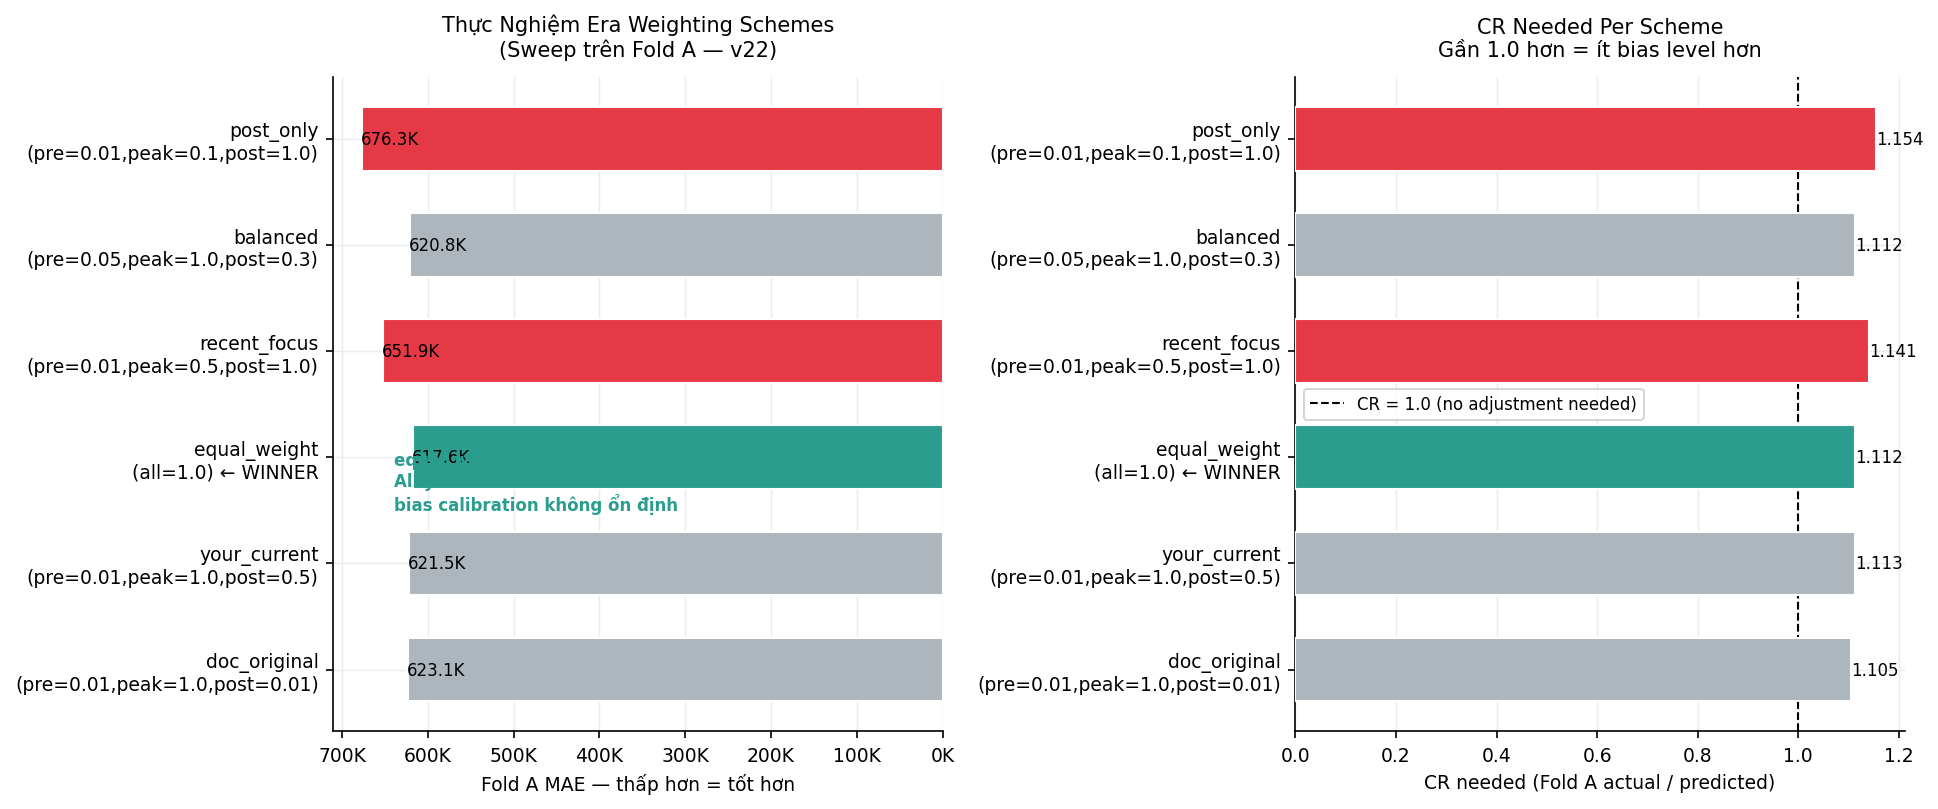
\includegraphics[width=\linewidth]{figures/modelling/fig11_era_weighting_experiment.png}
  \caption{Thực nghiệm era weighting: equal-weight thắng Fold A (617K)}
  \label{fig:era_exp}
\end{subfigure}
\hfill
\begin{subfigure}[b]{0.49\linewidth}
  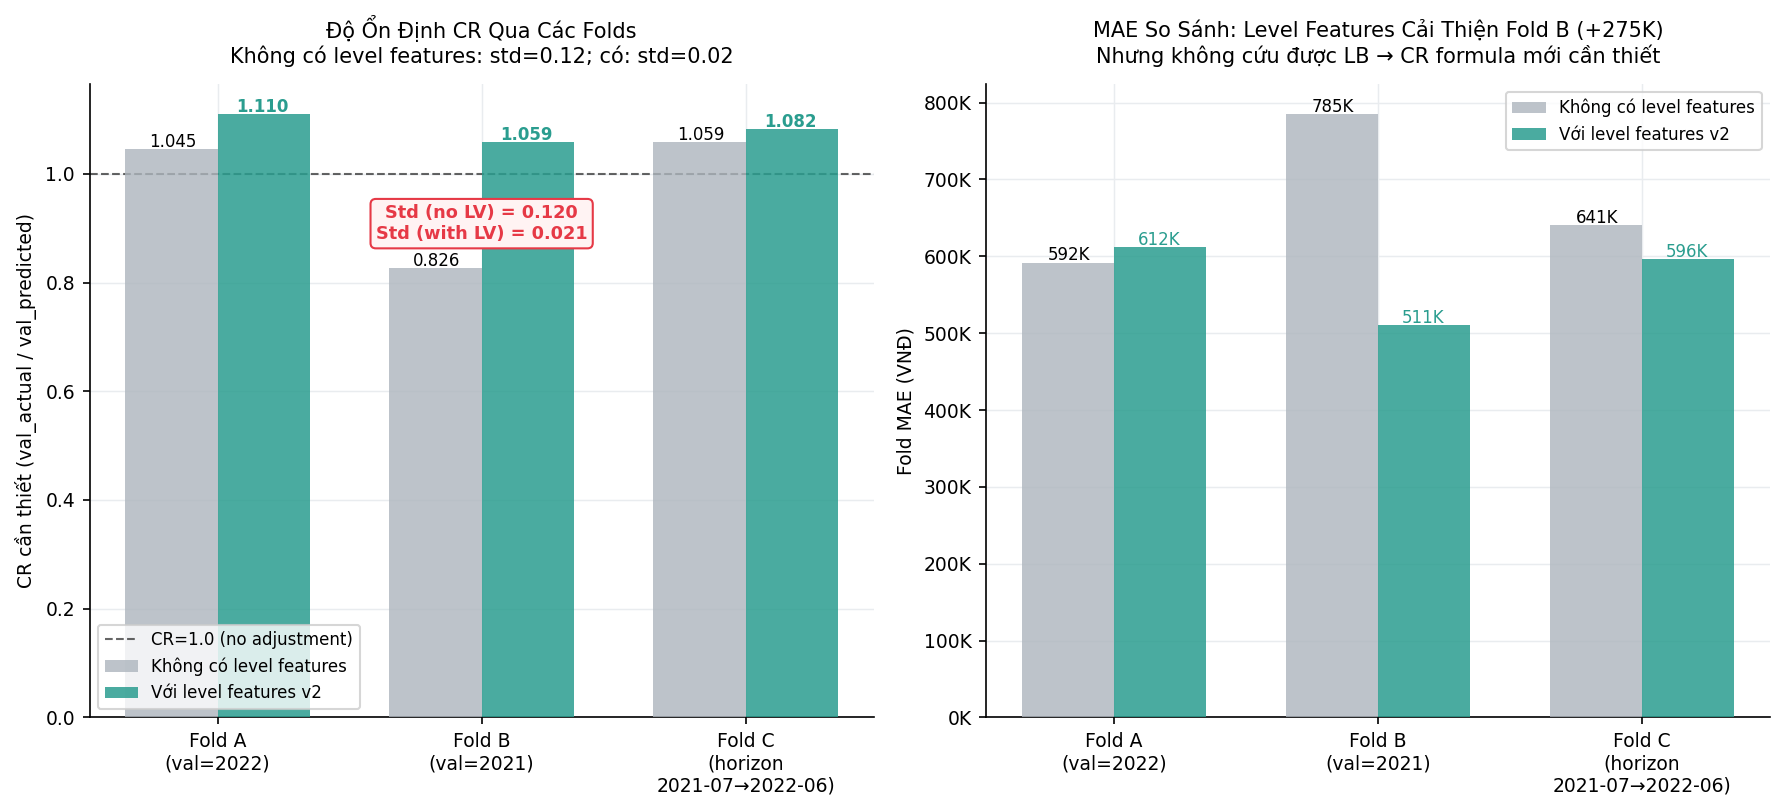
\includegraphics[width=\linewidth]{figures/modelling/fig13_fold_cr_consistency.png}
  \caption{Ổn định CR qua folds: không có level features std=0,12; có features std=0,02}
  \label{fig:fold_cr}
\end{subfigure}
\caption{Thực nghiệm era weighting và ổn định CR cross-fold.}
\end{figure}

\begin{figure}[h!]
\centering
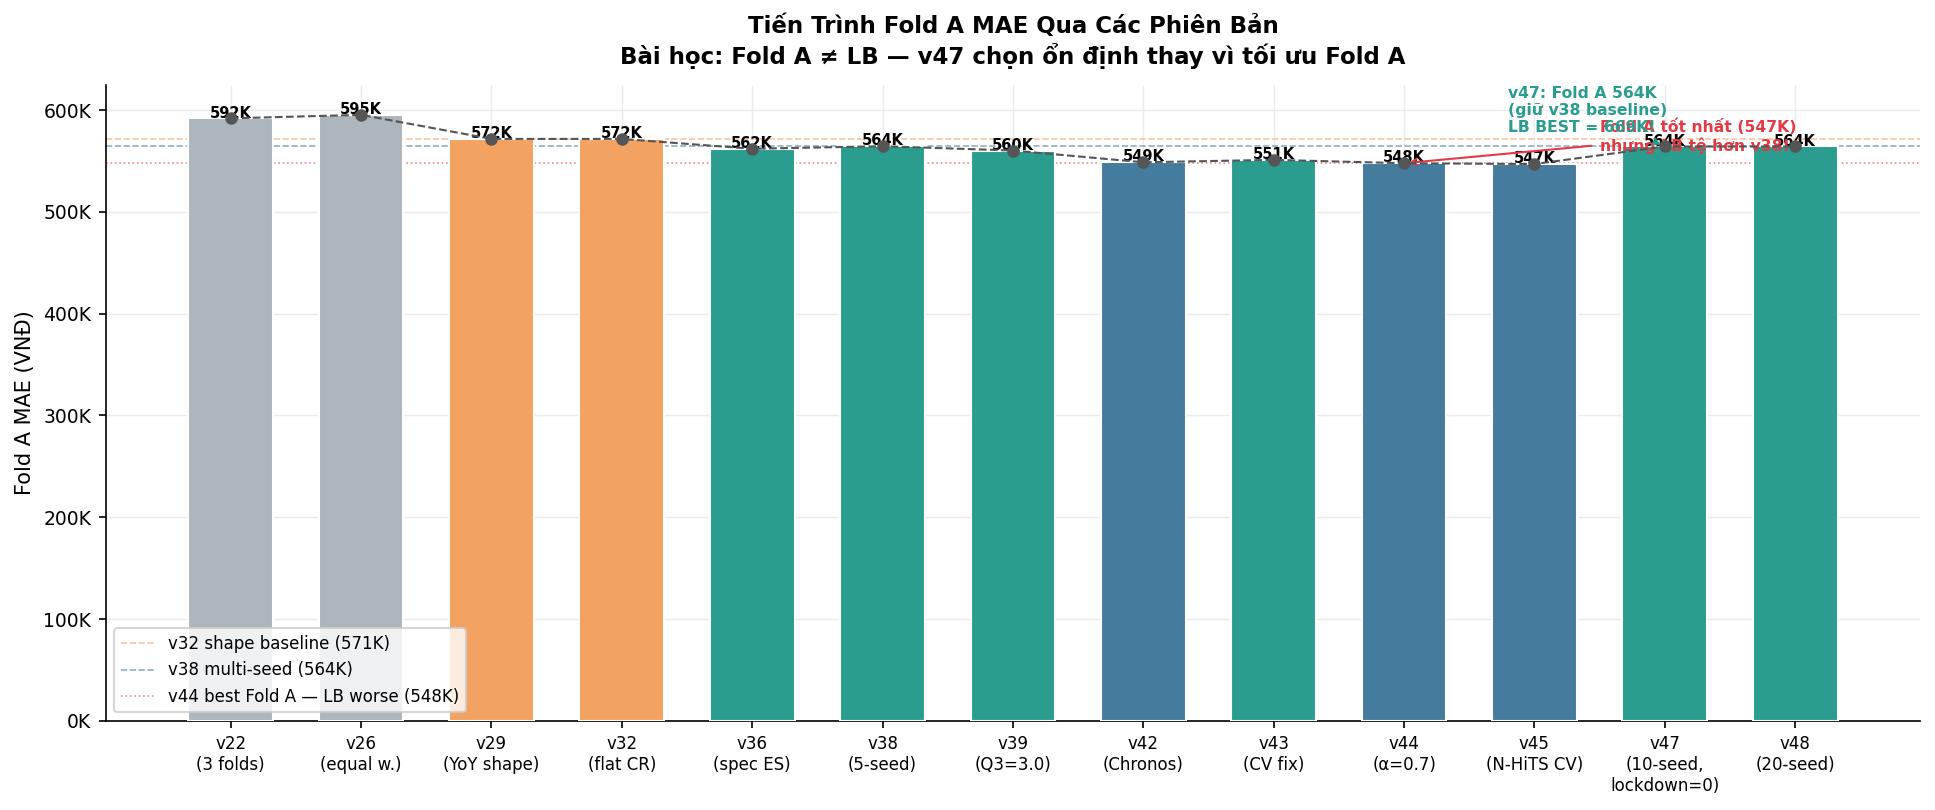
\includegraphics[width=0.8\linewidth]{figures/modelling/fig6_folda_mae_progression.png}
\caption{\textbf{Tiến trình Fold A MAE.} v44 đạt Fold A tốt nhất (548K) nhưng LB tệ hơn v38. v47 chủ động giữ Fold A $\approx$v38 (564K) và tối ưu bằng multi-seed + lockdown=0 — chiến lược đúng.}
\label{fig:folda_prog}
\end{figure}

% ===================================================================
\section{Phụ Lục C — SHAP Phân Tích Chi Tiết}
% ===================================================================

\begin{figure}[h!]
\centering
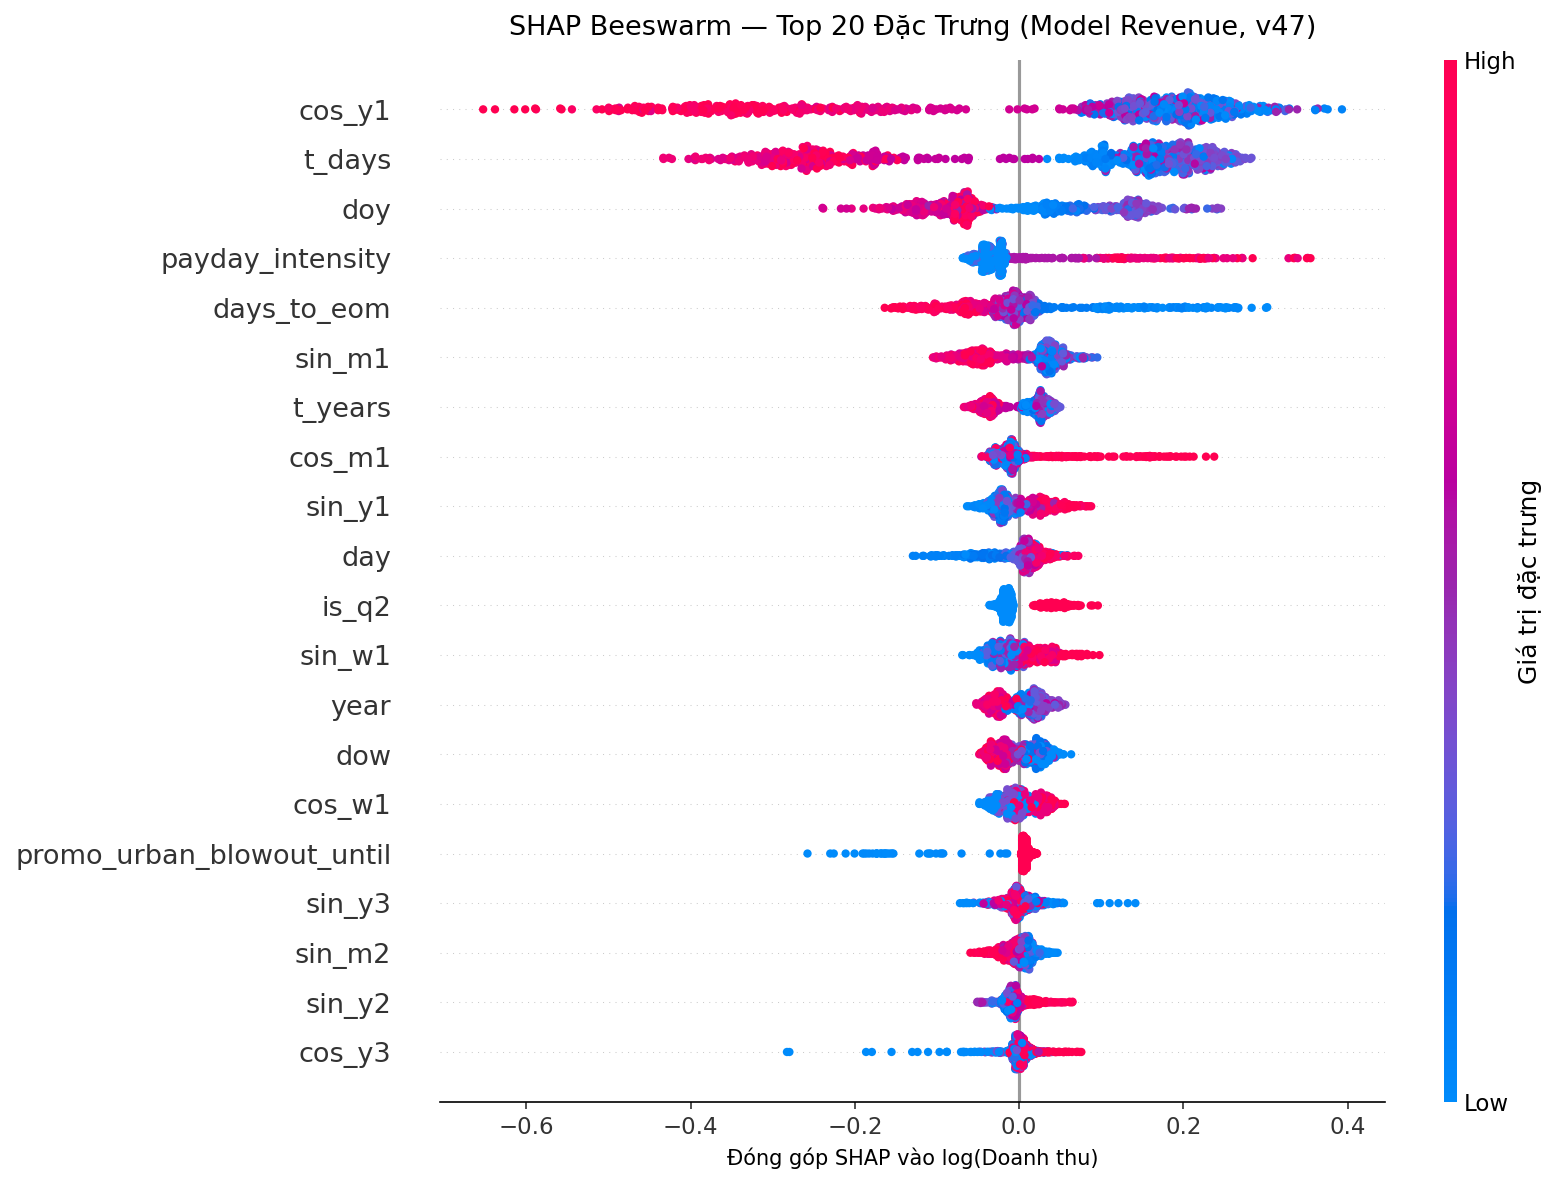
\includegraphics[width=\linewidth]{figures/shap/shap_summary_beeswarm.png}
\caption{\textbf{SHAP Beeswarm — Top 20 đặc trưng.} cos\_y1: màu đỏ (tháng 4–6) → SHAP $+0,3$; màu xanh (tháng 11–12) → SHAP $-0,6$. t\_days: màu xanh đậm (2014–2018) → SHAP $+0,4$; màu đỏ (2020–2022) → SHAP $-0,5$.}
\label{fig:beeswarm}
\end{figure}

\begin{figure}[h!]
\centering
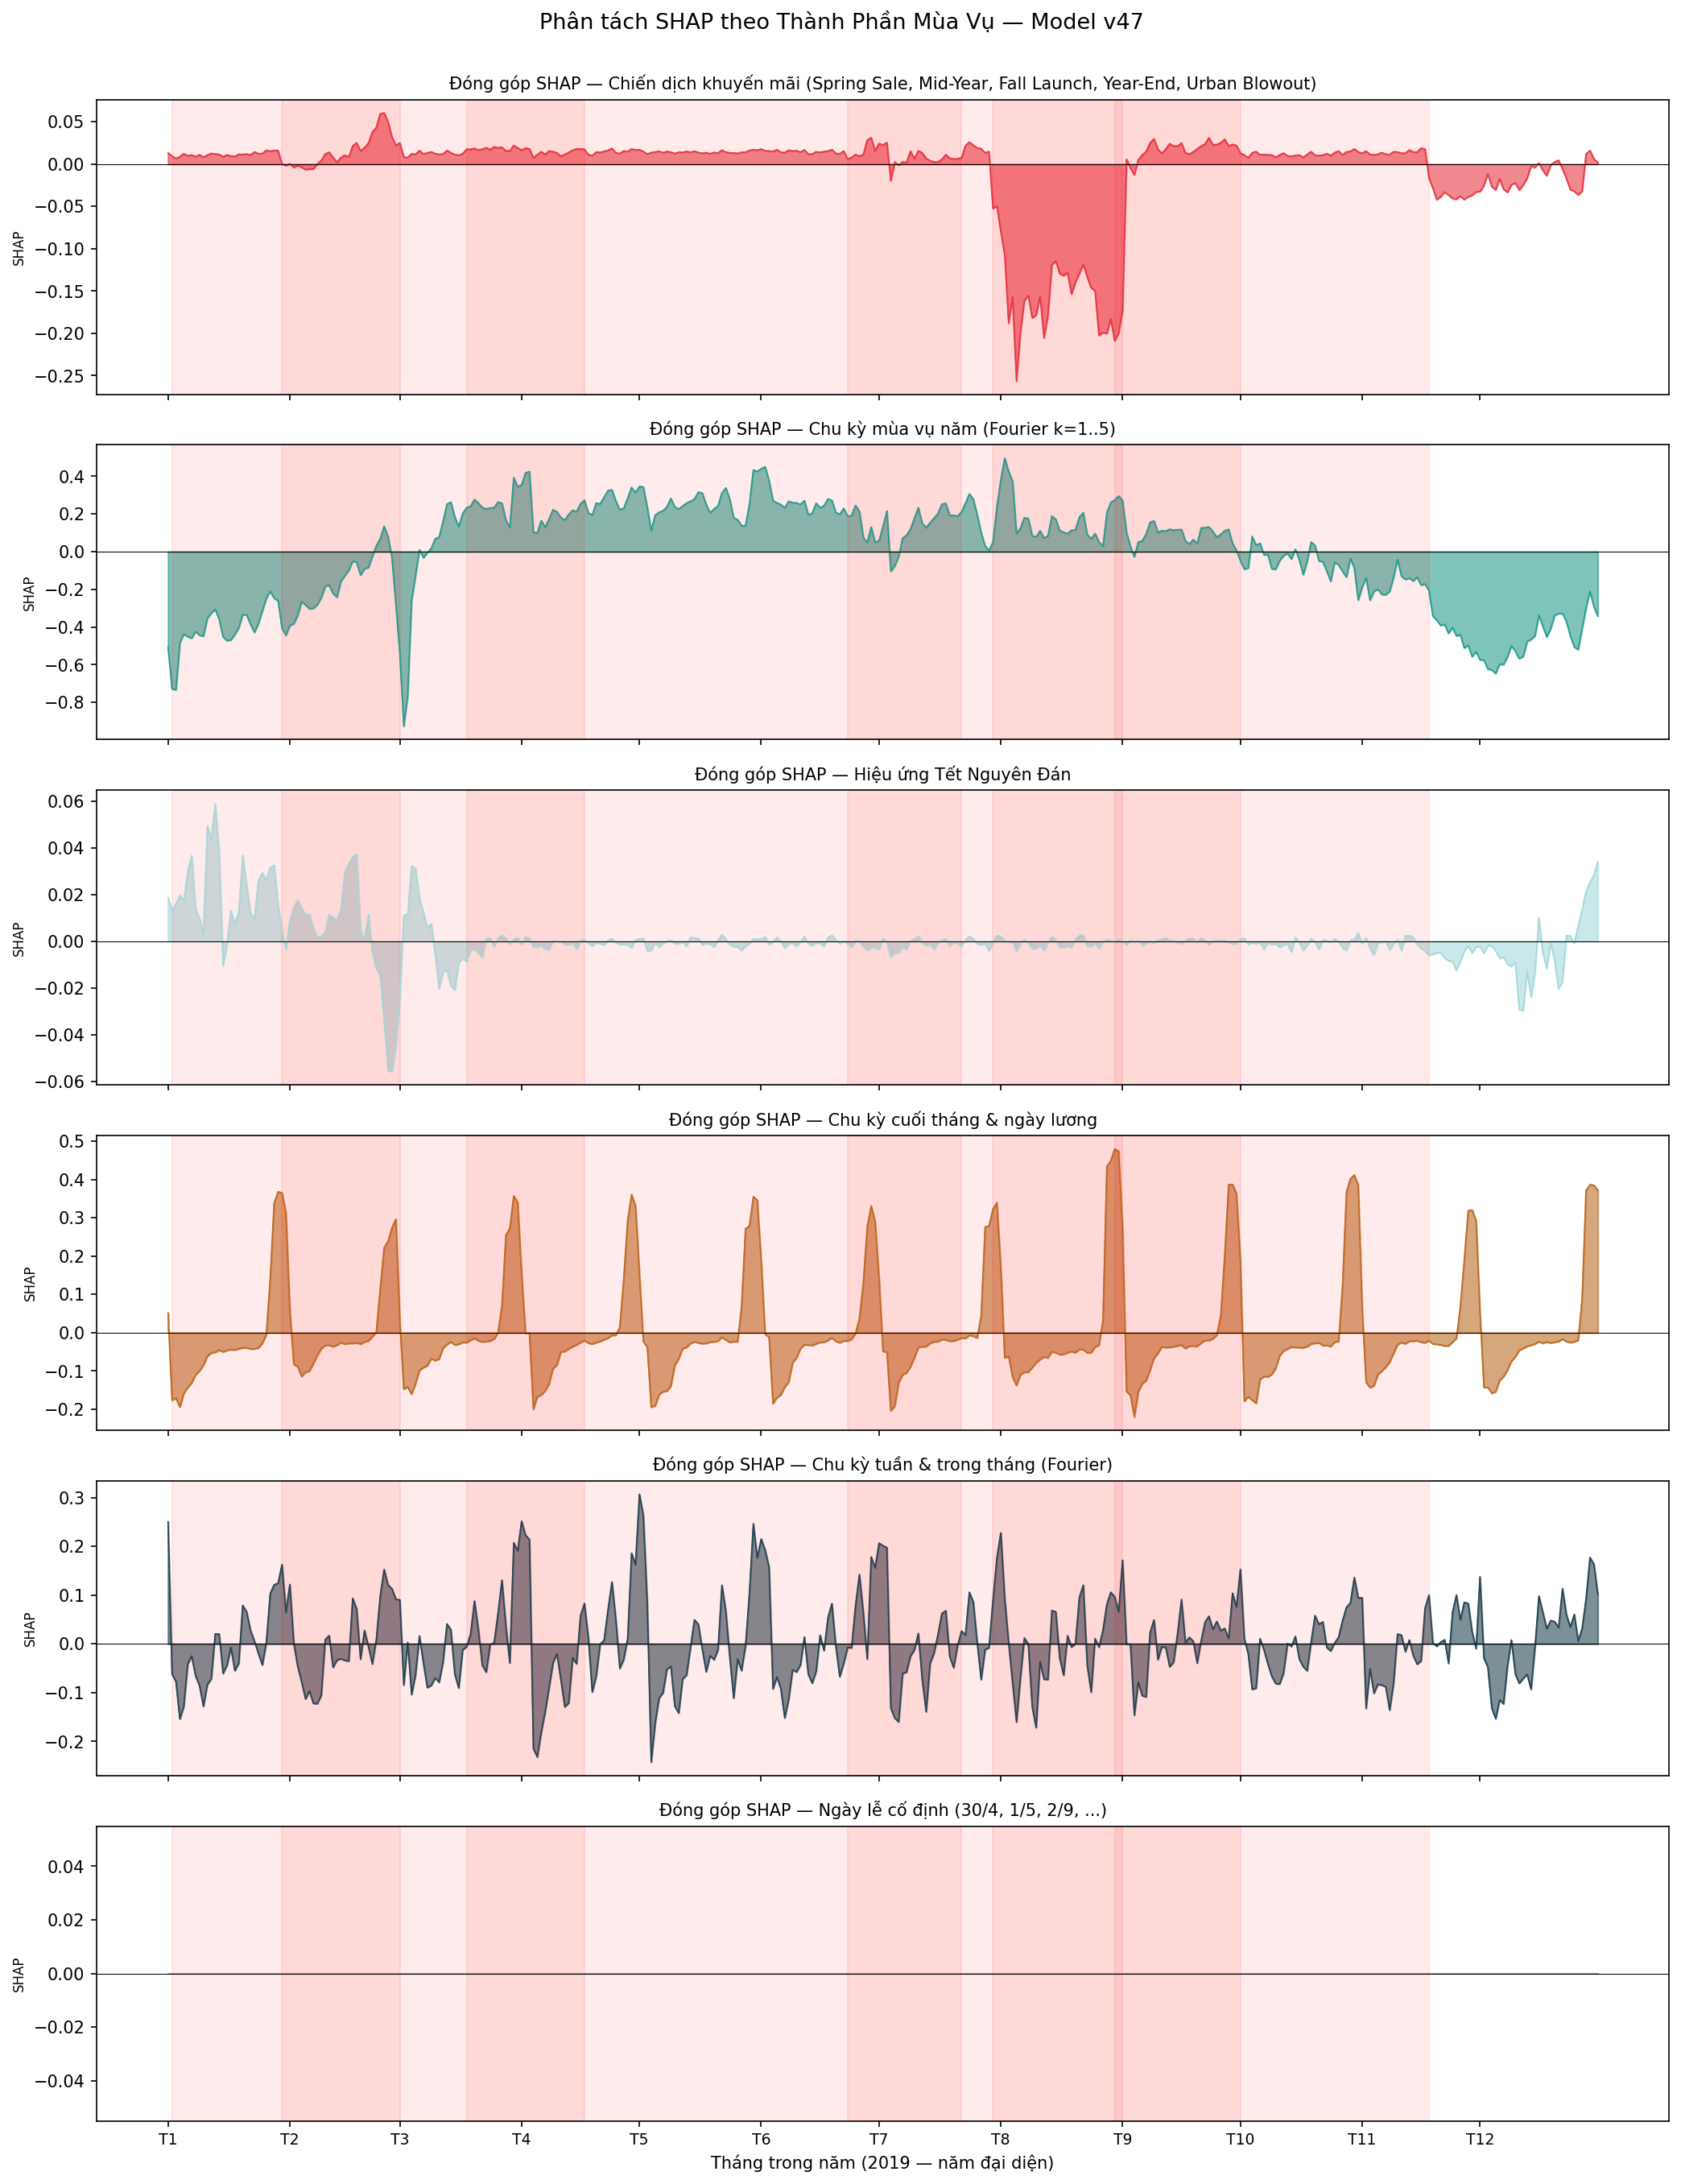
\includegraphics[width=\linewidth]{figures/shap/shap_seasonal_decomp.png}
\caption{\textbf{Phân tách SHAP theo thành phần mùa vụ (năm 2019).} Fourier năm có biên độ lớn nhất (±0,4–0,8). EOM/Lương: spike ±0,3–0,5 mỗi cuối tháng — lớn hơn Tết. Khuyến mãi Urban Blowout (T8): SHAP âm ($-$0,15 đến $-$0,25) — mô hình nhận diện đúng event margin-negative.}
\label{fig:shap_seasonal}
\end{figure}

\begin{figure}[h!]
\centering
\begin{subfigure}[b]{0.49\linewidth}
  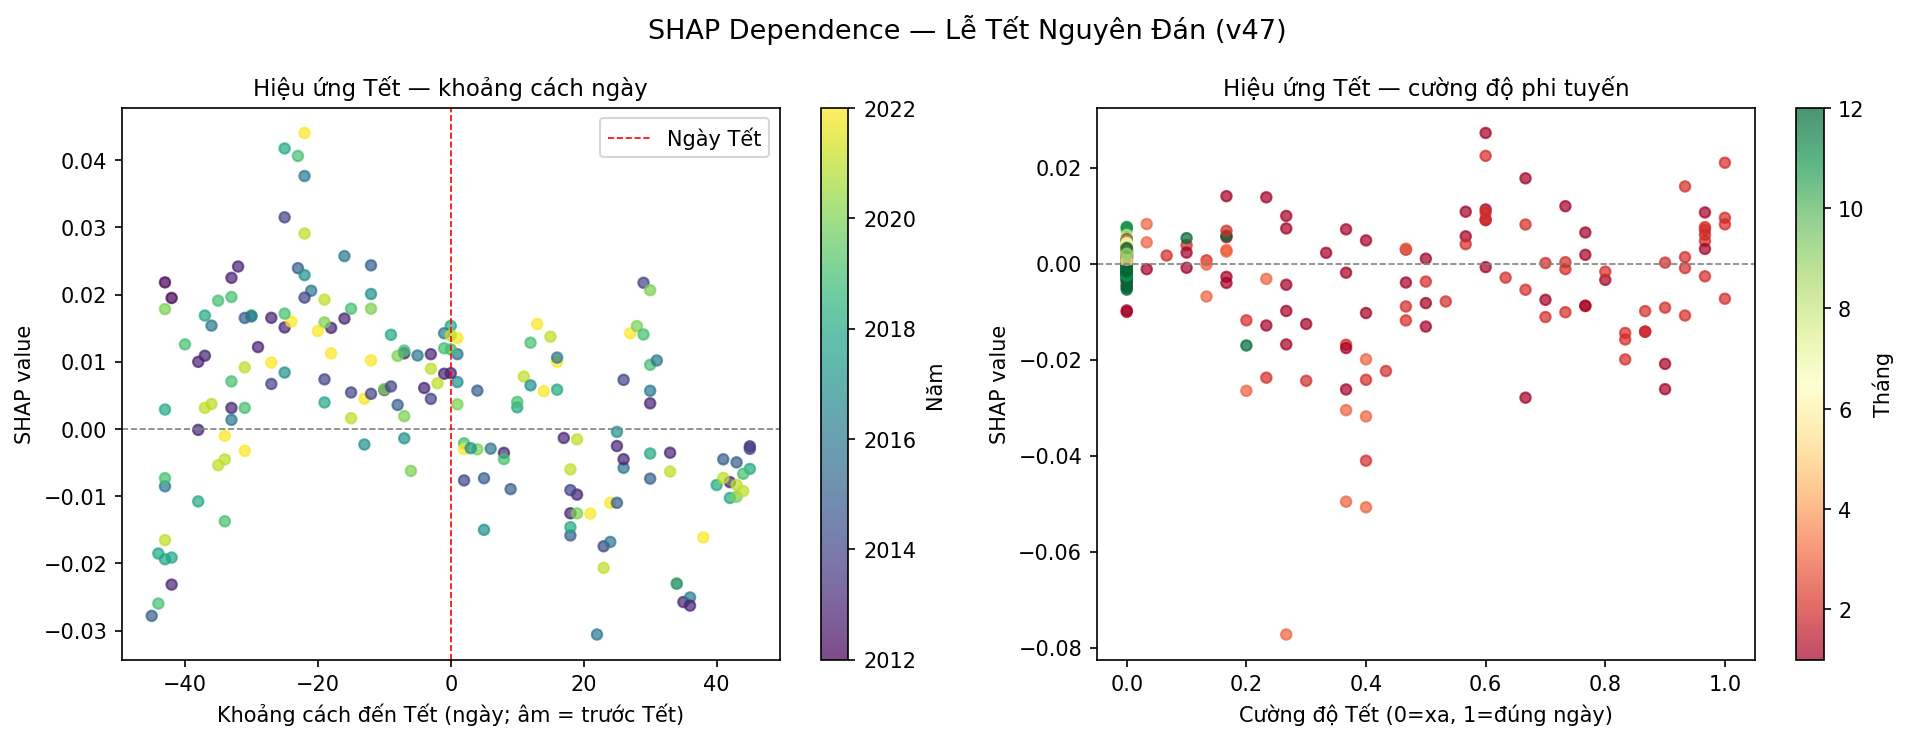
\includegraphics[width=\linewidth]{figures/shap/shap_dependence_tet.png}
  \caption{Hiệu ứng Tết: phi tuyến rõ rệt, dương trước Tết, âm ngay sau Tết}
  \label{fig:shap_tet}
\end{subfigure}
\hfill
\begin{subfigure}[b]{0.49\linewidth}
  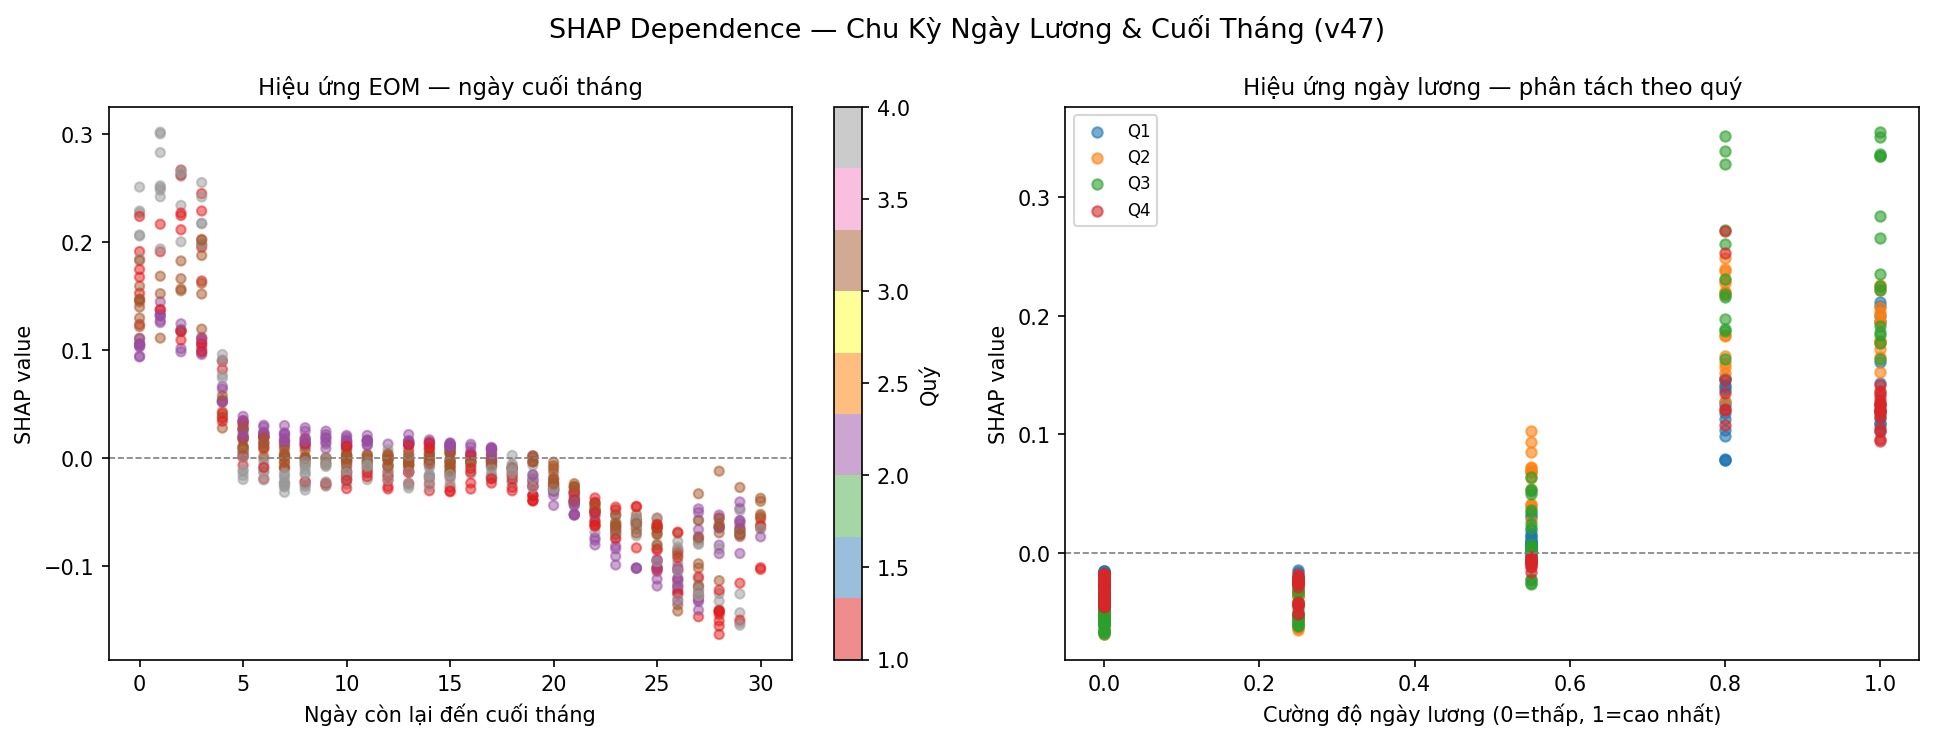
\includegraphics[width=\linewidth]{figures/shap/shap_dependence_eom_payday.png}
  \caption{EOM: SHAP giảm đơn điệu từ +0,25 (ngày 31) xuống $-$0,10 (đầu tháng)}
  \label{fig:shap_eom}
\end{subfigure}
\caption{SHAP Dependence plots: Tết và chu kỳ ngày lương.}
\end{figure}

\begin{figure}[h!]
\centering
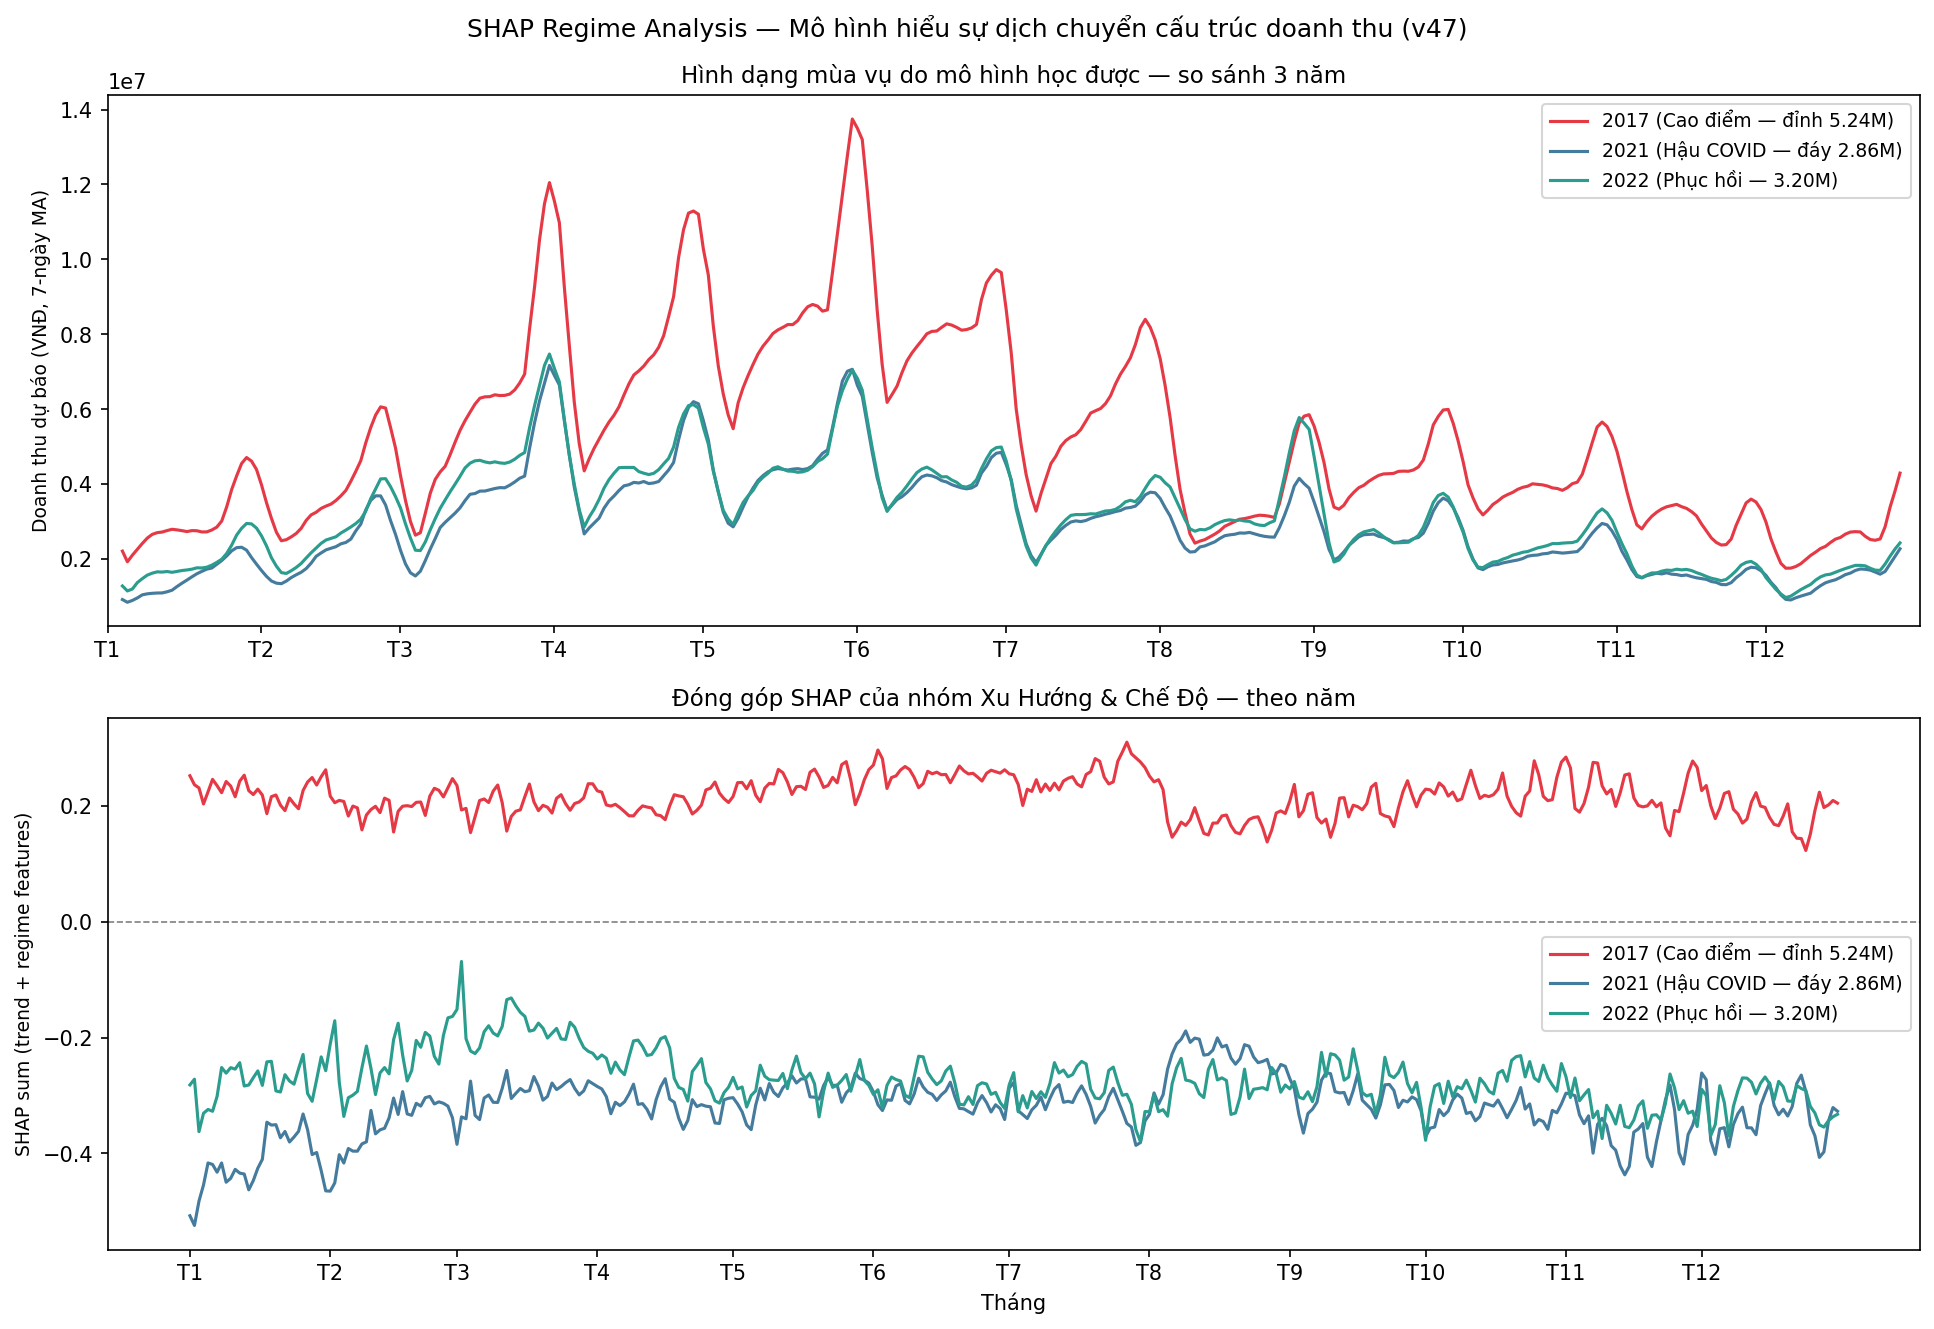
\includegraphics[width=0.9\linewidth]{figures/shap/shap_regime_comparison.png}
\caption{\textbf{SHAP phân tích regime.} Top: hình dạng mùa vụ 3 năm giống nhau nhưng level khác (2017: 8–14M, 2021–2022: 1–7M). Bottom: SHAP trend phân biệt đúng era — delta ~0,5 in log-space tương ứng 1,65× trong revenue scale, khớp với dữ liệu thực (5,24M/2,86M = 1,83×). Cơ sở cho CR = 1,2649.}
\label{fig:shap_regime}
\end{figure}

\begin{figure}[h!]
\centering
\begin{subfigure}[b]{0.49\linewidth}
  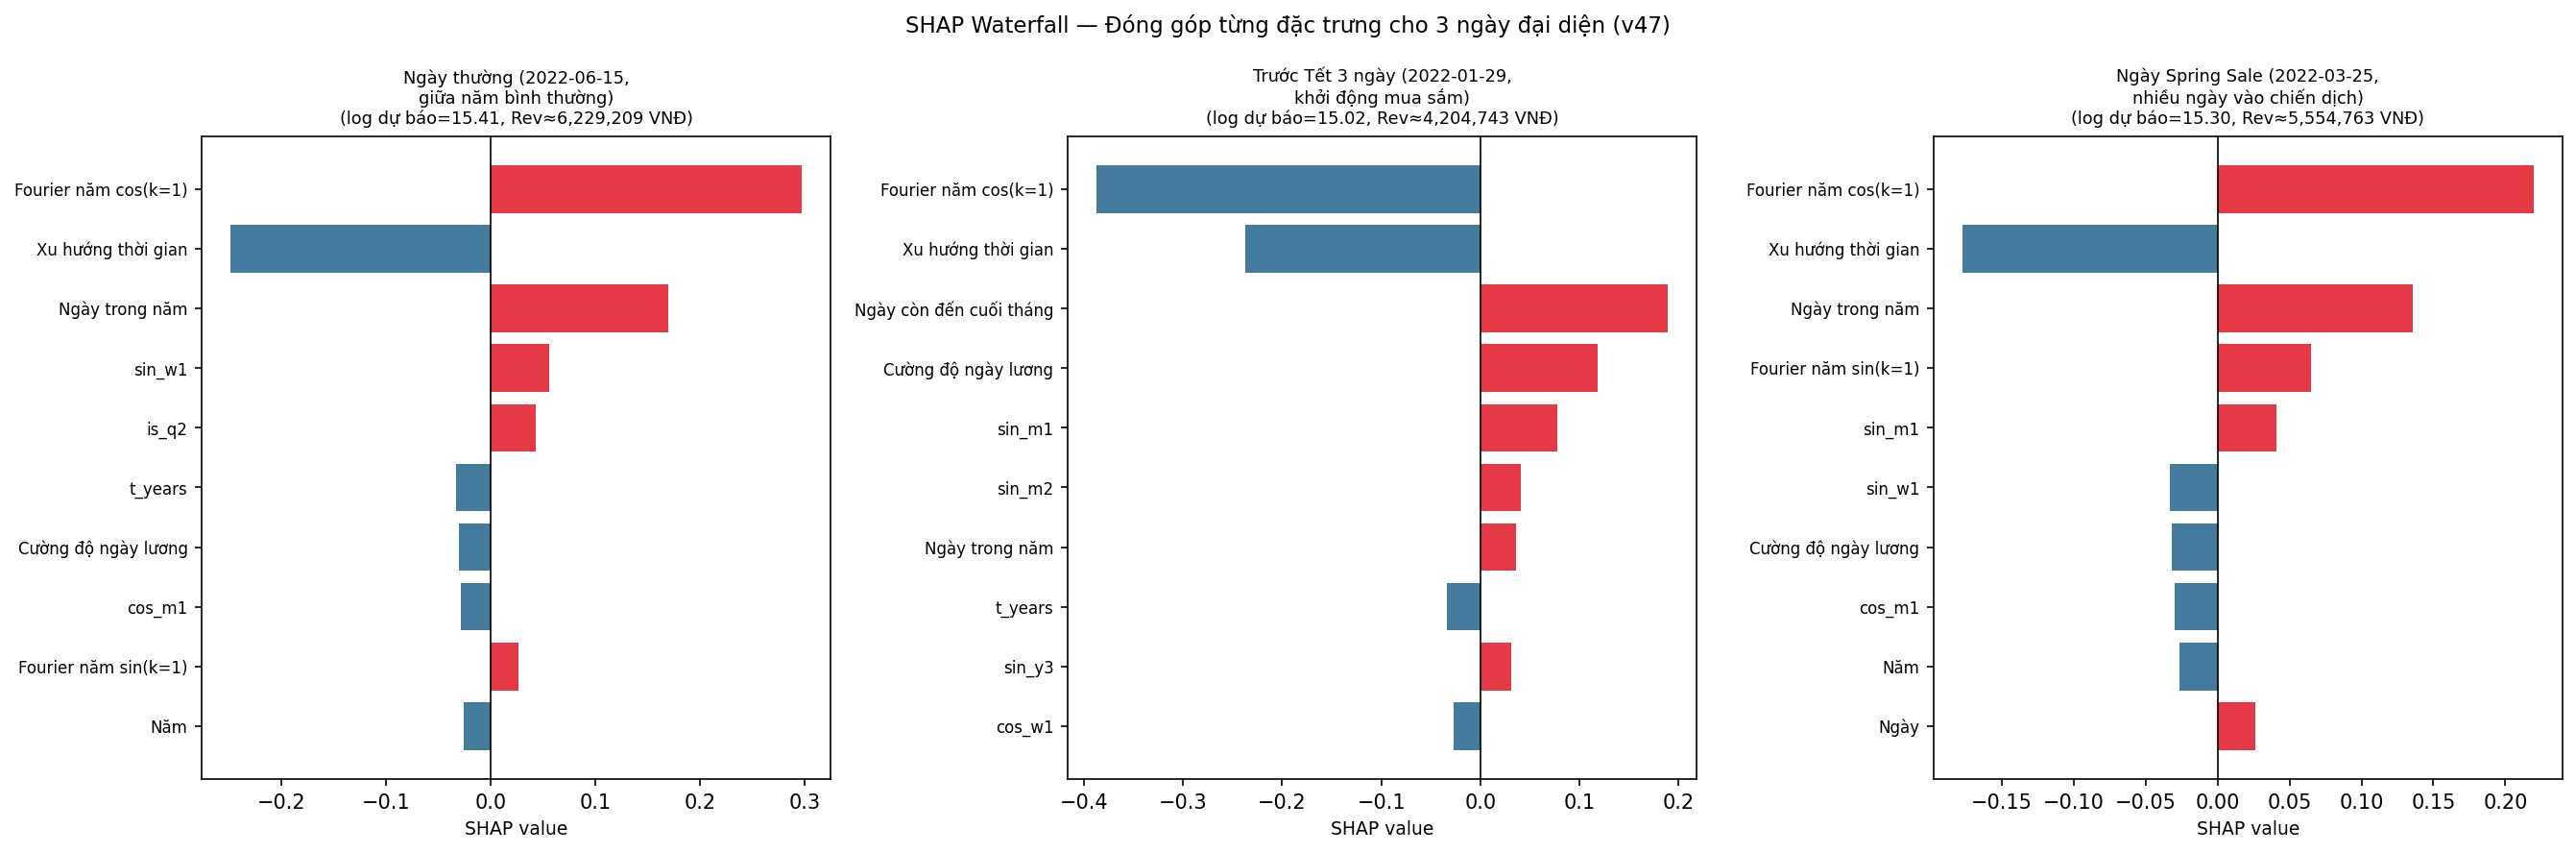
\includegraphics[width=\linewidth]{figures/shap/shap_waterfall_3days.png}
  \caption{Waterfall 3 ngày: thường, trước Tết 3 ngày, ngày Spring Sale}
  \label{fig:shap_waterfall}
\end{subfigure}
\hfill
\begin{subfigure}[b]{0.49\linewidth}
  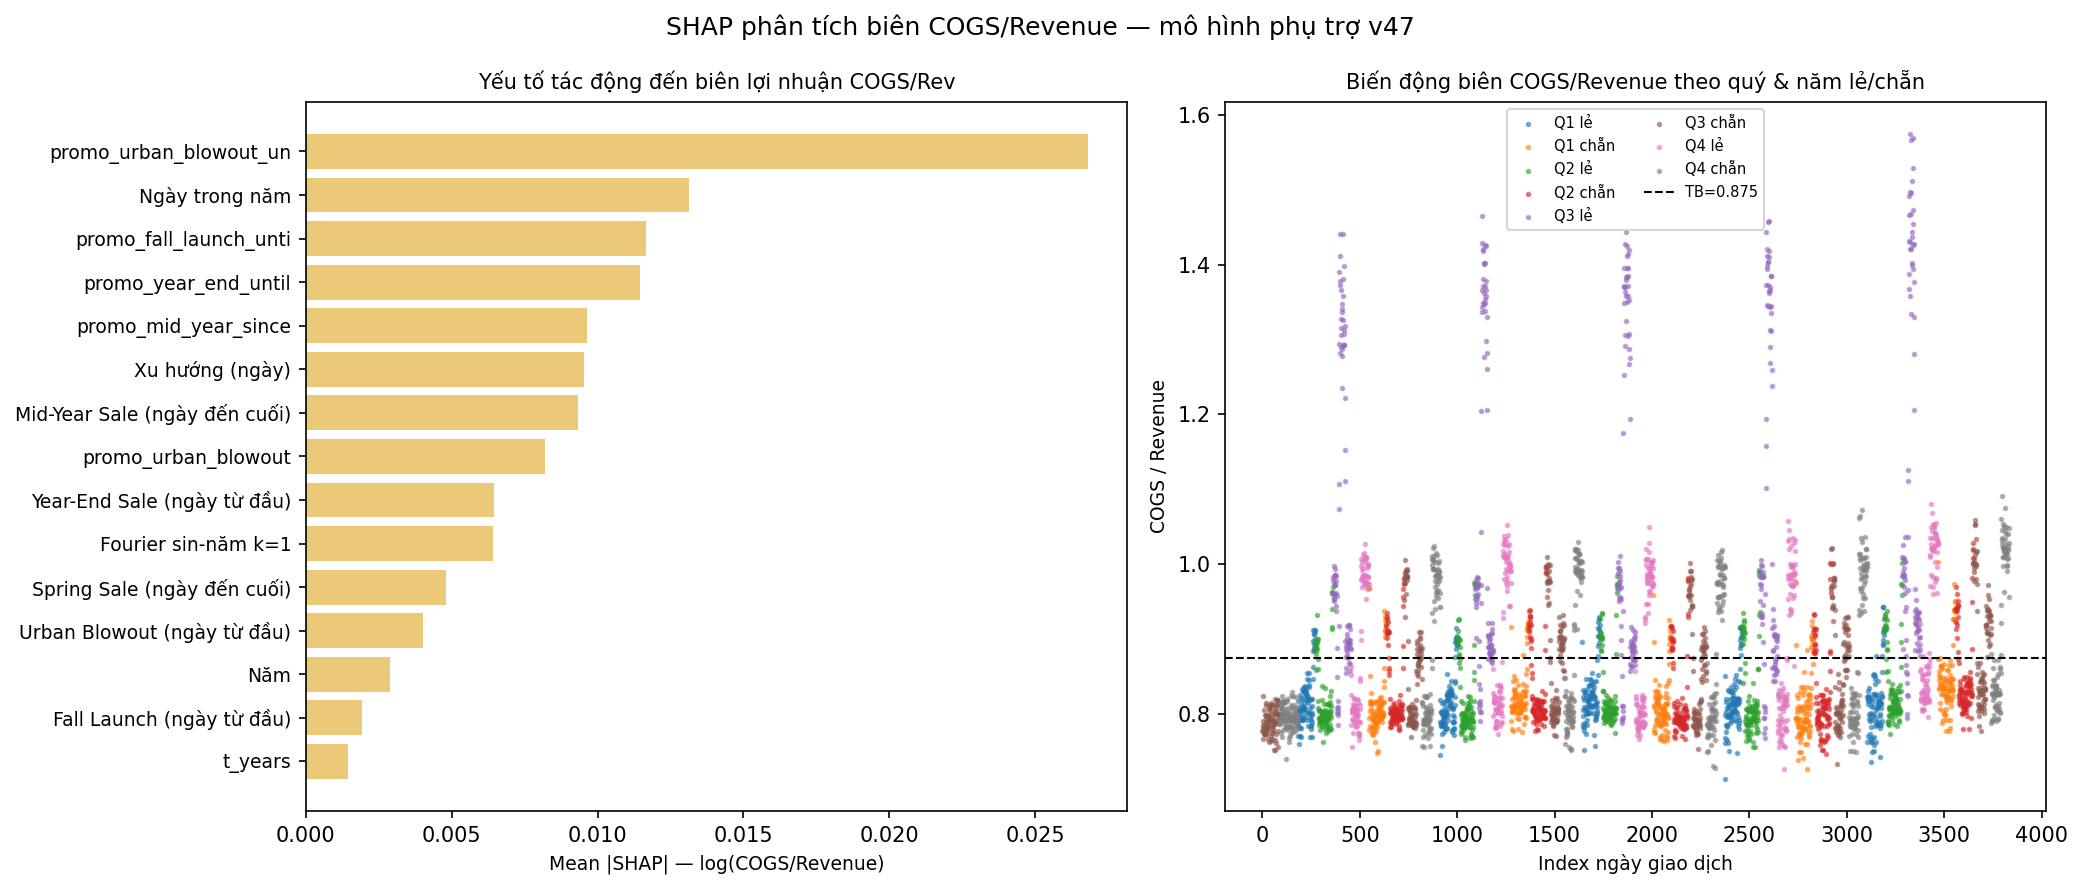
\includegraphics[width=\linewidth]{figures/shap/shap_margin_analysis.png}
  \caption{SHAP margin model: promo\_urban\_blowout\_until là driver chính của COGS/Rev}
  \label{fig:margin_shap}
\end{subfigure}
\caption{Waterfall đơn ngày và SHAP model margin COGS/Revenue.}
\end{figure}

\begin{figure}[h!]
\centering
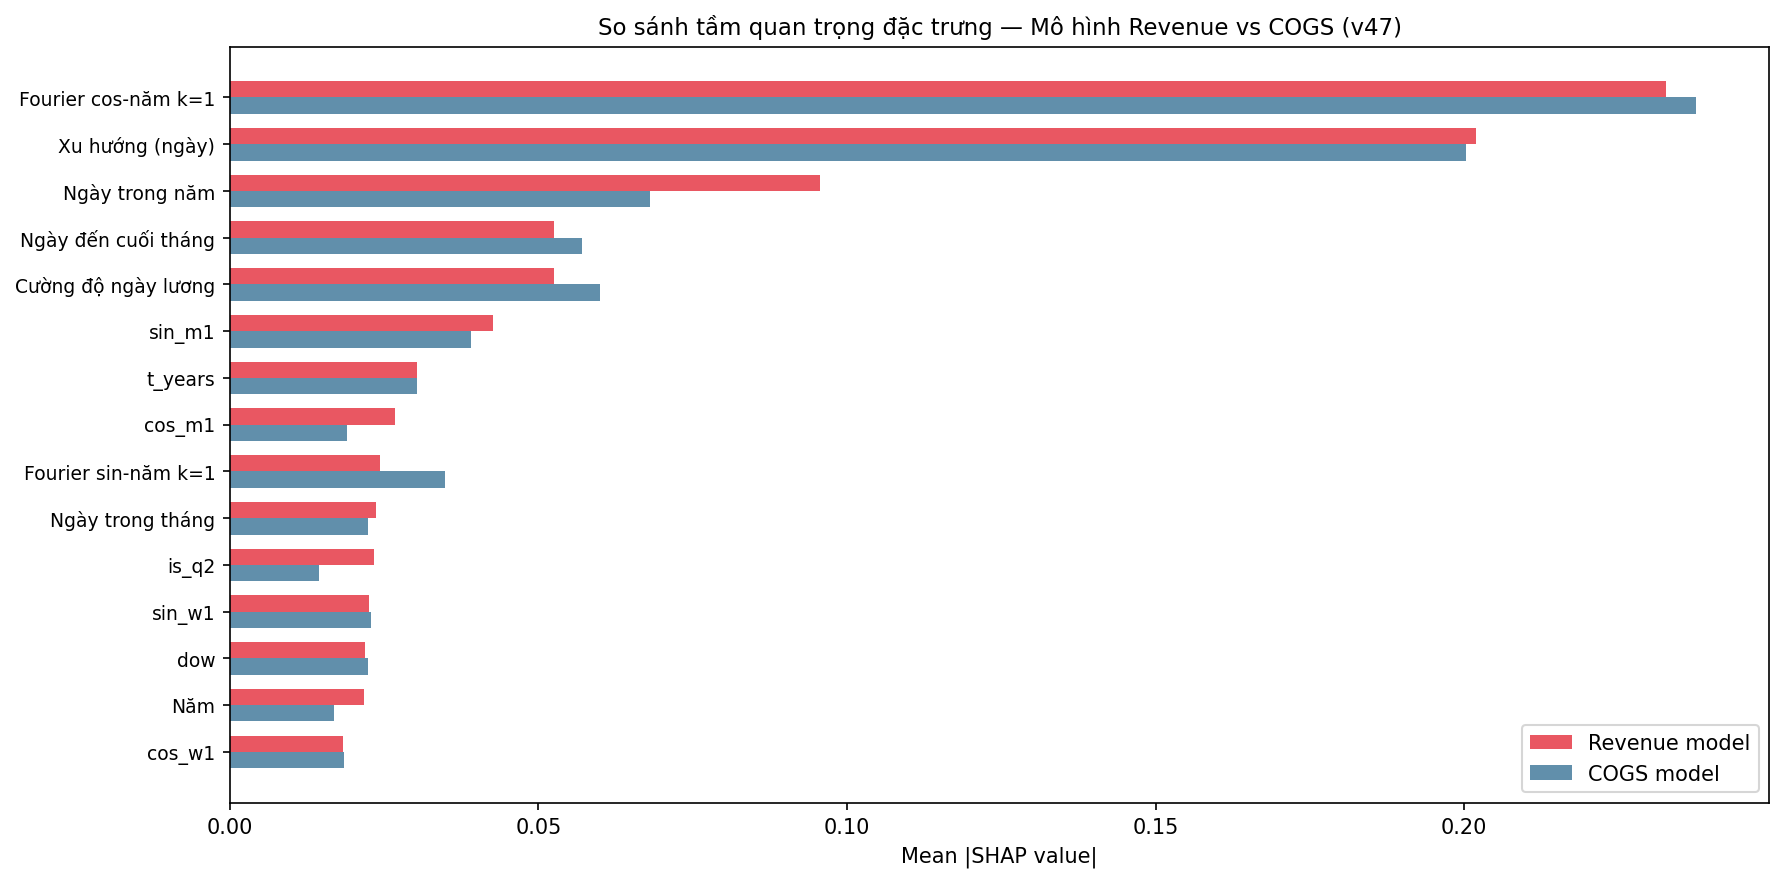
\includegraphics[width=\linewidth]{figures/shap/shap_cogs_vs_rev_comparison.png}
\caption{\textbf{So sánh SHAP Revenue vs COGS model.} Top-2 features giống hệt nhau (cos\_y1, t\_days). COGS nhạy cảm hơn với sin\_y1 (pha lệch 90°) — chi phí và doanh thu không cùng pha trong chu kỳ năm, biện hộ cho việc huấn luyện 2 mô hình riêng biệt.}
\label{fig:cogs_rev_shap}
\end{figure}

\begin{figure}[h!]
\centering
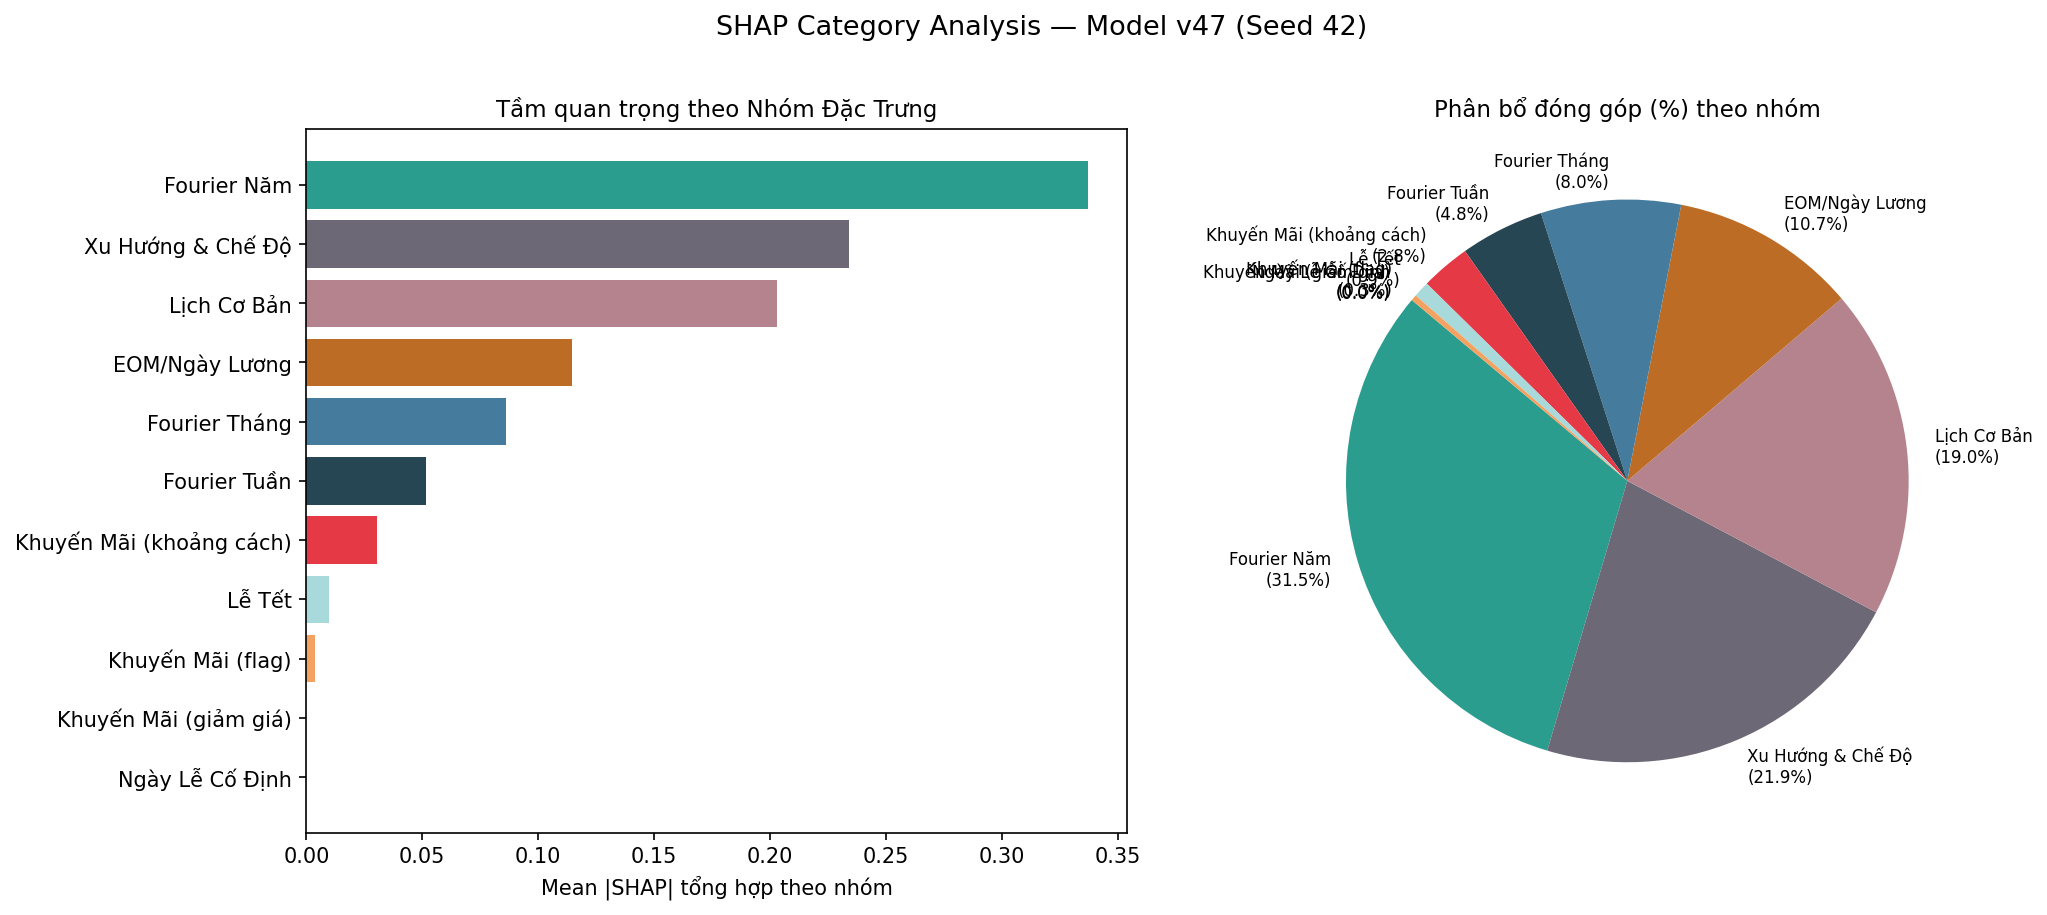
\includegraphics[width=0.85\linewidth]{figures/shap/shap_category_bar.png}
\caption{\textbf{SHAP theo nhóm đặc trưng.} Fourier Năm 31,5\% + Xu Hướng \& Chế Độ 21,9\% = 53,4\% tổng giải thích, xác nhận mô hình học đúng hai thành phần cốt lõi: shape và level.}
\label{fig:shap_cat}
\end{figure}

% ===================================================================
\section{Phụ Lục D — Thống Kê Mô Tả Chi Tiết \& Feature List}
% ===================================================================

\begin{figure}[h!]
\centering
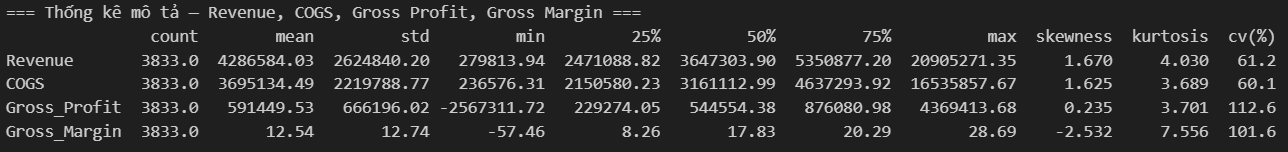
\includegraphics[width=\linewidth]{figures/eda/1.png}
\caption{Thống kê mô tả đầy đủ: Revenue, COGS, Gross Profit, Gross Margin — 3.833 quan sát.}
\label{fig:stats_full}
\end{figure}

\textbf{Danh sách 94 đặc trưng theo nhóm:}
\begin{itemize}
  \item \textbf{Fourier Năm (10):} sin\_y\{1..5\}, cos\_y\{1..5\}
  \item \textbf{Fourier Tuần (4):} sin\_w\{1,2\}, cos\_w\{1,2\}
  \item \textbf{Fourier Tháng (4):} sin\_m\{1,2\}, cos\_m\{1,2\}
  \item \textbf{Tết (9):} tet\_days\_diff, tet\_intensity, tet\_in\_7/14/30, tet\_before\_7, tet\_after\_7, tet\_on, tet\_post\_recovery
  \item \textbf{Khuyến mãi (24):} promo\_\{spring\_sale, mid\_year, fall\_launch, year\_end, urban\_blowout, rural\_special\} × \{flag, since, until, disc\}
  \item \textbf{EOM/Ngày lương (12):} days\_to\_eom, days\_from\_som, dim, is\_eom\_payday, payday\_intensity, is\_last\{1,2,3\}, is\_first\{1,2,3\}
  \item \textbf{Ngày lễ cố định (11):} hol\_\{new\_year, womens\_day, reunification, labor\_day, national\_day, vn\_womens\_day, dd\_1111, dd\_1212, christmas\_eve, christmas, hung\_kings\}
  \item \textbf{Xu hướng \& Chế độ (5):} t\_days, t\_years, regime\_pre2019, regime\_2019, regime\_post2019
  \item \textbf{Lịch cơ bản (15):} year, month, day, dow, doy, quarter, is\_weekend, is\_odd\_year, is\_q1/q2/q3/q4, q3\_odd\_year, hol\_black\_friday
\end{itemize}

\textbf{Hyperparameters LGB (v47):} objective=regression, metric=mae, learning\_rate=0,03, num\_leaves=63, min\_data\_in\_leaf=30, feature\_fraction=0,85, bagging\_fraction=0,85, bagging\_freq=5, lambda\_l2=1,0. Seeds: [42, 137, 314, 271, 999, 1234, 2718, 3141, 7777, 9999].

\textbf{Môi trường thực thi:} Kaggle Notebook (Python 3.10, NVIDIA P100 GPU 16GB). Thời gian chạy v47: $\approx$45 phút. Tất cả random seeds cố định. Không sử dụng dữ liệu ngoài bộ dữ liệu được cung cấp, ngoại trừ báo cáo tăng trưởng TMĐT MoIT 2022 (public).

\end{document}
